\chapter{Misc}

\section{ Sqrt-decomposition } % Traduzido
Sqrt-decomposition is a method or data structure that allows to perform some common operations (sum of subarray, finding the minimum / maximum, etc.) in $O (\sqrt {n})$, which is much faster than $O (n)$ for the trivial algorithm.

First, we describe the data structure for one of the simplest applications of this idea, then we show how to generalize it to deal with some other problems, and finally, consider some other use of this idea: to partition the input queries in ``sqrt-blocks''.

\subsection{ Data structure based on sqrt-decomposition }

\textbf{Problem.} Given an array $a [0 \ldots n-1]$, you want to have a data structure that can find the sum of elements $a [l \ldots r]$ for arbitrary $l$ and $r$ in $O (\sqrt {n})$.

\subsubsection{ Description }

The main idea of sqrt-decomposition is the following: Divide array $a$ into blocks of length about $\sqrt {n}$, and in each block $i$ precalculate the sum $b [i]$ of the elements in it.

We can assume that the length of a block and the number of them is equal to the same number - the square root of $n$, rounded up:

$s = \left \lceil \sqrt {n} \right \rceil,$

then the array $a []$ is divided into blocks like this:

$\underbrace{a[0]a[1]\ldots a[s-1]}_{b[0]}\underbrace{a[s]\ldots a[2\cdot s-1]}_{b[1]}\ldots\underbrace{a[(s-1)\cdot s]\ldots a[n]}_{b[s-1]}$

Note that the last block may contain less than $s$ elements (if $n$ is not divisible by $s$) - but it is not important.

Thus, for each block $k$ we know its sum $b [k]$:

$b[k]=\sum_{i=k\cdot s}^{\min(n-1,(k+1)\cdot s-1)}a[i]$

So, suppose we have these values $b_k$ previously calculated (to do this, $O (n)$ operations is enough). How they can give the answer to the sum of a request $(l, r)$? Note that if the segment $[l; r]$ is long enough, then it will contain a few whole blocks, which we already have their sum. The remaining part of the segment $[l; r]$ will be only the two blocks that fall into it only partially (if any), and in these we will use a trivial summation algorithm.

Illustration

$\ldots\overbrace{a[l]\ldots a[(k+1)\cdot s-1]\underbrace{a[(k+1)\cdot s]\ldots a[(k+2)\cdot s-1]}_{b[k+1]}\ldots\underbrace{a[(p-1)\cdot s]\ldots a[p\cdot s-1]}_{b[p-1]}a[p\cdot s]\ldots a_{r}}^{{\rm sum=?}}\ldots$

In this figure, it is clear that in order to calculate the sum of the segment $[l \ldots r]$, it is necessary to sum the elements of the two "tails": $[l \ldots (k +1) \cdot s-1]$ and $[p \cdot s \ldots r]$ and sum the values $b [i]$ in all blocks from $k +1$ to $p-1$:

$\sum_{i=l}^{r}a[i]=\sum_{i=l}^{(k+1)\cdot s-1}a[i]+\sum_{i=k+1}^{p-1}b[i]+\sum_{i=p\cdot s}^{r}a[i]$

(Note: This calculation is wrong when $k = p$ : In this case, some of the items will be added up twice, in which case you simply sum the elements from $l$ to $r$ instead)

Thus we reduced a significant number of operations. Indeed, the size of each of the "tails" does not exceed the length of the block $s$ and the number of blocks also does not exceed $s$. Since we chose $s \approx \sqrt {n}$, then to calculate the sum of the segment $[l \ldots r]$ we need only $O (\sqrt {n})$ operations.

\subsubsection{ Implementation }

We start with a simple implementation:

\begin{verbatim}
int n ;
vector < int > a(n);
 
int len =(int)sqrt(n +.0)+ 1 ; // block size and the number of blocks
vector < int > b(len);
for(int i = 0 ; i < n ; ++ i )
    b[i / len]+ = a[i];
 
// response to requests
for(;;){
    int l, r ; // reads the input data - the next request
    int sum = 0 ;
    for(int i = l ; i <= r ; )
        if(i % len == 0 && i + len - 1 <= r){
            // if i indicates the beginning of the block entirely in [l; r]
            sum + = b[i / len];
            i + = len ;
        }
        else {
            sum + = a[i];
            ++ i ;
        }
} 
\end{verbatim}
The drawback of this implementation is that it uses a lot of unneeded divisions (which run much slower than the other operations). Instead, you can calculate the indexes of blocks $c_l$ and $c_r$ where are the boundaries $l$ and $r$ are respectively, and then make a loop through the blocks from $c_l +1$ to $c_r-1$, handling the "tails" in the blocks $c_l$ and $c_r$. In addition, the case $c_l = c_r$ is special and requires a separate treatment:

\begin{verbatim}
int sum = 0 ;
int c_l = l / len,   c_r = r / len ;
if(c_l == c_r )
    for(int i = l ; i <= r ; ++ i )
        sum + = a[i];
else {
    for(int i = l, end =(c_l + 1)* len - 1 ; i <= end ; ++ i )
        sum + = a[i];
    for(int i = c_l + 1 ; i <= c_r - 1 ; ++ i )
        sum + = b[i];
    for(int i = c_r * len ; i <= r ; ++ i )
        sum + = a[i];
} 
\end{verbatim}
\subsubsection{ Other tasks }

We considered the problem of finding the sum of the elements in a subarray. This task can be expanded a little: let me also \textbf{change} individual elements in $a$. Indeed, if an element $a_i$ is changed it is sufficient to update the value of $b [k]$ in the block in which the element is located ($k = i / len$).

$b [k] + = a [i] - old \_a [i]$

Additionaly, the same technique applies to the problem of finding the \textbf{minimal/maximal} element in a subarray. If you want to allow changes of individual elements, you have to recalculate the value $b_k$ from the corresponding block but this time you need to iterate in the elements of the block using $O (len) = O (\sqrt {n})$ operations.

Similarly, sqrt-decomposition can be applied to many similar problems: finding the number of zero elements, the first nonzero element, counting the number of certain elements, etc.

There is also a whole class of problems which allows \textbf{changes in a subarray of elements}, adding or modifying the elements of the array at some subsegments.

For example, consider the following two types of queries: adding a value $\delta$ to the elements of a segment $[l; r]$ and returning the value of an individual element $a_i$. Then let $b_k$ be the value to be added to all items in block $k$  (i.e, initially all $b_k = 0$), then the query "addition" will need to perform an addition to all the elements $a_i$ from the "tails" and increment all the values $b_i$ for the blocks lying entirely in the interval $[l \ldots r]$. The answer to the other query is going to be $a_i + b_k$ where $k = i / len$. Thus, the addition operation will be performed in $O (\sqrt {n})$ and the request for an element in $O (1)$.

Finally, you can use both types of operations: modify items in a interval and response to queries in a interval. Both types of operations will be carried out in $O (\sqrt {n})$. For this we will need to have two "block" arrays $b$ and $c$ - one for addition value in a block and the other for the sum.

There are other applications that can use sqrt-decomposition. For example, we can solve the problem of \textbf{maintaining a set of numbers} with the ability to add/delete numbers, test if a number is in the set. To solve this problem it is necessary to store the numbers in sorted order, stored in a blocks of $\sqrt {n}$ numbers in each. When adding or removing elements, it will be necessary to 	 ``rebalance'' the blocks, transferring numbers from the beginning/end of some blocks into the beginning/end of the neighboring blocks.

\subsection{ Sqrt-decomposition for queries }

We now consider very different ideas about the use of sqrt-decomposition.

Suppose that we have some problem in which we are given some input data, and then are asked to perform $k$ commands/requests, each of which have to process and issue a response. We consider the case where the requests are queries (do not change the state of the data, but only asks for some information) and updates (i.e, affecting the data defined initially).

Some specific tasks can be quite complex, and processing dynamic updates and queries can be challenging. On the other hand, solving the ``off-line'' version of the problem, i.e, where there are no update operations, but only queries is often much easier. Assume that we \textbf{can solve the ``offline'' version of the} problem, i.e. build some data structure with time $B(n)$ that can answer queries, but cannot handle modifying queries.

Then \textbf{we split the input data in blocks} (denote the block length by $s$). At the beginning, for each block we build a data structure for the "off-line" version of the problem using the data at the start of the block.

Now we'll start taking requests and handle each one. If the request is to modify, then skip it, otherwise refer to the data structure for the offline version of the problem, but before \textbf{process all modifying queries in the corresponding block}. The algorithm to apply these updates should be fast enough - in time $O (s)$ or a little worse, we denote this time $Q (s)$.

So, if we have $m$ requests, you will need time $B (m) \frac {m} {s} + m Q (s)$ to process them. The value of $s$ should be selected based on the functions $B()$ and $Q()$. For example, if $B (m) = O (m)$ and $Q (s) = O (s)$, the best choice would be $s \approx \sqrt {m}$, and the resulting asymptotics will be $O (m \sqrt {m})$.

Since the above argument is too abstract, we give some examples of problems to which this sqrt-decomposition applies.

\subsubsection{ Example task: Adding the interval }

\textbf{Problem. } Given an array of numbers $a [1 \ldots n]$, there are two types of queries: find value in $i$-th position of the array, and add a number $x$ to each array element in an interval $a [l \dots r]$.

Although this problem can be solved without receiving requests to the partition into blocks, we present it here - as a simple and intuitive application of this method.
% Fim tradução
So, we split the input into a series of requests $\sqrt {m}$ (Where $m$ - The number of requests). At the beginning of the first block of requests to build any structures do not, just keep an array $a []$. We go now to request the first block. If the current request - a request the addition, it is still miss it. If the current request - request to read the value of a position $i$, First it's just take as a response value $a [i]$. Then go through all missed in this block requests the addition, and for those of them, which gets $i$ We apply them to the current increase in response.

Thus, we have learned to respond to requests for requesting time $O (\sqrt {m})$.

It remains only to note that at the end of each block of requests, we have to apply all modifying queries that block to the array $a []$. But it's easy to make for $O (n)$ - Enough for every request the addition of $(l, r, x)$ note in the secondary array at $l$ number $x$ And at the point $r +1$ - The number of $-X$ And then go through the array, adding a running total of the array $a []$.

Thus, the final decision will be asymptotic $O (\sqrt {m} (n + m))$.

\subsubsection{ Example problem: disjoint-set-union with division }

There is an undirected graph with $n$ vertices and $m$ edges. Request comes in three forms: add an edge $(X_i, y_i)$, Remove the edge $(X_i, y_i)$ And check whether or not connected vertices $x_i$ and $y_i$ way.

If no removal requests, then the solution would be a data structure known disjoint-set-union (a system of disjoint sets). However, if there is a remote task much more complicated.

Done as follows. At the beginning of each block of queries see which edges in the block will be removed, and immediately \textbf{remove} them from the graph. Now we construct a system of disjoint sets (dsu) on the resulting graph.

As we now have to respond to another request from the current block? Our system of disjoint sets "knows" all the edges, except those that are added / removed in the current block. However, the removal of dsu we do not need - we pre removed all such edges of the graph. Thus, all that can be - is more, add ribs, which can be a maximum $\sqrt {m}$ pieces.

Therefore, in response to the current query requesting we can just let crawl across to the connected components dsu, which has worked for $O (\sqrt {m})$ Because we are only in the consideration $O (\sqrt {m})$ edges.

\subsection{ Off-line subsegments queries and versatile array sqrt heuristics }

Consider another interesting variation ideas sqrt-decomposition.

Suppose we have a problem in which there is an array of numbers, and there are requesting queries of the form $(l, r)$ - To learn something about the subsegments $a [l \ldots r]$. We believe that the requests are not modified, and are known to us in advance, i.e. task - off-line.

Finally, we introduce the last \textbf{limitation,} we believe that we can quickly recalculate prompted when the left or right edge of one. Ie If we knew the answer to a query $(l, r)$, You can quickly find the answer to your inquiry $(l +1, r)$ or $(l-1, r)$ or $(l, r +1)$ or $(l, r-1)$.

We now describe the \textbf{generic heuristics} for all these problems. Sort the requests for the pair: $(l ~ {\rm div} ~ \sqrt {n}, r)$. Ie We sorted the requests by number sqrt-block, in which lies the left end, and at equality - at the right end.

Now consider the group requests with the same value $l ~ {\rm div} ~ \sqrt {n}$ and see how we can handle it. All such requests have ordered the right edge, and, therefore, we can just start with a blank portion $[l; l-1]$, And time after time increases by one the right border - eventually respond to all such requests.

A good \textbf{example} for this heuristic is a challenge: see how many different numbers in the segment array $[l; r]$. This problem is difficult to address classical methods.

Slightly more complicated version of this problem is a problem with one of the rounds Codeforces.


\section{ Fenwick tree }
\textbf{Fenwick tree} - a data structure, a tree on the array with the following properties:

1) allows us to calculate the value of a reversible operation G on any interval [L; R] in the time \textbf{O (log N);}

2) to adjust the value of any element of \textbf{O (log N);}

3) requires \textbf{O (N) memory,} or more precisely, the same number as there are an array of N elements;

4) is easily generalized to the case of multi-dimensional arrays.

The most common use of wood Fenwick - to calculate the amount of the interval, i.e. function G (X1,..., Xk) = X1 +... + Xk.

Fenwick tree was first described in the article "A new data structure for cumulative frequency tables" (Peter M. Fenwick, 1994).

\subsection{ Description }
For ease of description, we assume that the operation of G, on which we build a tree - this \textbf{amount.}

Suppose given an array A [0.. N-1]. Fenwick tree - an array \textbf{T} [0.. N-1], each element of which is kept a sum of some elements of the array A:

\begin{verbatim}
  \textbf{T i = the sum of A j} for all \textbf{F (i) <= j <= i,} 
\end{verbatim}
where F (i) - a function, which we define later.

Now we can write the \textbf{pseudo-code} for computing the sum of the functions on the interval [0; R] for the function changes the cell:

\begin{verbatim}
 int sum (int r)
 {
     int result = 0;
     while (r>= 0) {
         result + = t [r];
         r = f (r) - 1;
     }
     return result;
 }

 void inc (int i, int delta)
 {
     for all j, for which F (j) <= i <= j
     {
         t [j] + = delta;
     }
 } 
\end{verbatim}
The sum function works as follows. Instead of going through all elements of the array A, it moves through the array T, making the "jump" through the segments where possible. First, it adds to the response value of the sum on the interval [F (R); R], then takes the sum of the segment [F (F (R) -1); F (R) -1], and so on, until it reaches the zero.

Function inc moves in the opposite direction - in the direction of increasing index, updating sum value T j only for those items for which it is needed, i.e. for all j, for which F (j) <= i <= j.

Obviously, the choice of the function F depends on both the speed of operations. Now we consider a function that would achieve a logarithmic performance in both cases.

\textbf{Determine the value of F (X)} as follows. Consider the binary representation of the number and look at its least significant bit. If it is zero, then F (X) = X. Otherwise, the binary representation of X ends with a group of one or more units. Replace all the units of the group for the zeros, and assign that number value of the function F (X).

This rather complex description is of a very simple formula:

\begin{verbatim}
  \textbf{F (X) = X & (X +1),} 
\end{verbatim}
where A - is a bitwise logical 'AND'.

It is easy to see that this formula corresponds to the verbal description of the functions given above.

We just have to learn how to quickly find those numbers j, for which F (j) <= i <= j.

However, it is not difficult to make sure that all numbers can be obtained from i j successive changes of the rightmost (least significant) zeros in binary representation. For example, for i = 10, we find that j = 11, 15, 31, 63, etc.

Ironically, such an operation (replacing the youngest zero to unity) also corresponds to a very simple formula:

\begin{verbatim}
  \textbf{H (X) = X | (X +1),} 
\end{verbatim}
where | - is a bitwise logical "OR".

\subsection{ Fenwick tree implementation for the sum in 1D case }
\begin{verbatim}
 vector <int> t;
 int n;

 void init (int nn)
 {
     n = nn;
     t.assign (n, 0);
 }

 int sum (int r)
 {
     int result = 0;
     for (; r>= 0; r = (r & (r +1)) - 1)
         result + = t [r];
     return result;
 }

 void inc (int i, int delta)
 {
     for (; i <n; i = (i | (i +1)))
         t [i] + = delta;
 }

 int sum (int l, int r)
 {
     return sum (r) - sum (l-1);
 }

 void init (vector <int> a)
 {
     init ((int) a.size());
     for (unsigned i = 0; i <a.size(); i++)
         inc (i, a [i]);
 } 
\end{verbatim}

\subsection{ Fenwick tree implementation for minimum of 1D case }
It should be immediately noted that, as the tree Fenwick allows you to find the function at an arbitrary interval [0; R], then we will not be able to find a minimum in the interval [L; R], where L> 0. Furthermore, all the changing values ​​should only occur in the direction of decreasing (again, does not work because the function call min). This is a significant limitation.

\begin{verbatim}
 vector <int> t;
 int n;

 const int INF = 1000 * 1000 * 1000;

 void init (int nn)
 {
     n = nn;
     t.assign (n, INF);
 }

 int getmin (int r)
 {
     int result = INF;
     for (; r>= 0; r = (r & (r +1)) - 1)
         result = min (result, t [r]);
     return result;
 }

 void update (int i, int new_val)
 {
     for (; i <n; i = (i | (i +1)))
         t [i] = min (t [i], new_val);
 }

 void init (vector <int> a)
 {
     init ((int) a.size());
     for (unsigned i = 0; i <a.size(); i++)
         update (i, a [i]);
 } 
\end{verbatim}
\subsection{ Fenwick tree implementation for the sum of 2D case }
As already noted, the tree Fenwick easily generalized to the multidimensional case.

\begin{verbatim}
 vector <vector <int>> t;
 int n, m;

 int sum (int x, int y)
 {
     int result = 0;
     for (int i = x; i>= 0; i = (i & (i +1)) - 1)
         for (int j = y; j>= 0; j = (j & (j +1)) - 1)
             result + = t [i][j];
     return result;
 }

 void inc (int x, int y, int delta)
 {
     for (int i = x; i <n; i = (i | (i +1)))
         for (int j = y; j <m; j = (j | (j +1)))
             t [i][j] + = delta;
 } 
\end{verbatim}
\section{ System of disjoint sets }
This article discusses the structure of the \textbf{data, "a system of disjoint sets"} (in English "disjoint-set-union", or simply "DSU").

This data structure provides the following features. Initially, there are several elements, each of which is a separate (his own) set. One operation can \textbf{combine any two sets,} and you can also \textbf{request, in what} is now \textbf{the set of} the specified item. Also, the classic version, introduced another operation - the creation of a new element, which is placed in a separate set.

Thus, the basic interface of the data structure consists of only three steps:

${\rm make \_set} (x)$ - \textbf{Adds} a new element $x$ By placing it in a new set consisting of one him.
${\rm union \_sets} (x, y)$ - \textbf{Brings together} two of the sets (a set in which the element is $x$ And set, in which the element is $y$ ).
${\rm find \_set} (x)$ - \textbf{Returns in what many} are specified item $x$. In fact, when it returns one of the elements of the set (called \textbf{representative} or \textbf{leader} (in English literature "leader")). This representative is chosen in each set of the very structure of the data (and may change over time, namely, after the call ${\rm union \_sets}()$ ).
For example, if the call ${\rm find \_set}()$ for any two elements returned the same value, it means that these elements are in the same set, and otherwise - in the different sets.

Described by the following data structure allows each of these operations in nearly $O (1)$ on average (more on the asymptotics below after the description of the algorithm).

Also in one of the sub-article describes an alternative embodiment of the DSU, allowing to achieve asymptotic $O (\log n)$ an average of one request for $m \ge n$, And at $m >> n$ (Ie $m$ much more $n$)- And at the time $O (1)$ an average of the request (see "Storage DSU as an explicit list of sets").

\subsection{ Building an efficient data structure }

We first determine the form in which we will store all the information.

Set of elements we will store in the form of \textbf{trees:} one tree corresponds to a single set. The root of the tree - is representative (leader) of the set.

When implemented, this means that we lead array ${\rm parent}$ In which each element we store a reference to its parent in the tree. For the roots of trees, we assume that their ancestors - they (i.e. the link loops in this place).

\subsubsection{ Naive implementation }

We can already write the first implementation of a system of disjoint sets. It will be quite inefficient, but then we will improve it with the help of two methods, resulting in a nearly constant time.

So, all the information about the sets of elements stored at us with an array of ${\rm parent}$.

To create a new item (operation ${\rm make \_set} (v)$ ), We simply create a tree rooted at the top $v$ Noting that her ancestors - is she.

To combine the two sets (operation ${\rm union \_sets} (a, b)$ ), We first find the leaders of the set in which the $a$ And set, in which the $b$. If leaders are matched, then do not do anything - it means that the set is already been merged. Otherwise, you can simply indicate that the ancestor of the vertices $b$ is $a$ (Or vice versa) - thus joining one tree to another.

Finally, the implementation of the search operation leader(${\rm find \_set} (v)$)Is simple: we ascend from the top of the ancestors $v$ Until you get to the root, i.e., while the reference to the ancestor is not in himself. This can be suitably implemented recursively (in particular it will be convenient later, in connection with adding optimizations).

\begin{verbatim}
void make_set(int v){
    parent[v]= v ;
}
 
int find_set(int v){
    if(v == parent[v])
        return v ;
    return find_set(parent[v ]);
}
 
void union_sets(int a, int b){
    a = find_set(a);
    b = find_set(b);
    if(a ! = b )
        parent[b]= a ;
} 
\end{verbatim}
However, this implementation of disjoint sets very \textbf{inefficient.} It is easy to construct examples where, after several unions of sets get a situation that a lot of - a tree, degenerated into a long chain. As a result, each call ${\rm find \_set}()$ will work on this test during the order of the depth of the tree, i.e., for $O (n)$.

This is very far from the asymptotics, we were going to get (constant time). Therefore, we consider two optimizations that allow (even applied separately) streamline.

\subsubsection{ Heuristic path compression }

This heuristic is designed to speed up ${\rm find \_set}()$.

It lies in the fact that when, after a call ${\rm find \_set} (v)$ we find the desired leader $p$ set, then remember that at the top $v$ and all passed on the way of points - this is the leader $p$. The easiest way to do this by redirecting their ${\rm parent} []$ this peak $p$.

Thus, an array of ancestors ${\rm parent} []$ meaning is somewhat different: it is now \textbf{compressed array of ancestors,} i.e. for each vertex there can be stored direct ancestor, and ancestor ancestor ancestor ancestor ancestor, etc.

On the other hand, it is clear that you can do to these pointers ${\rm parent}$ always point to the leader: the way in step ${\rm union \_sets}()$ would have to update the leaders in $O (n)$ elements.

Thus, the array ${\rm parent} []$ it should be treated as an array of ancestors, perhaps partially compressed.

The new implementation of the operation ${\rm find \_set}()$ is as follows:

\begin{verbatim}
int find_set(int v){
    if(v == parent[v])
        return v ;
    return parent[v]= find_set(parent[v ]);
} 
\end{verbatim}
This simple implementation does what was intended, first by a leader of recursive calls is set, and then, in the promotion of the stack, this leader is assigned to the links ${\rm parent}$ passed for all elements.

Implement this operation is possible and non-recursive, but then have to carry out two runs on wood: first find the desired leader, the second - to put it to all of the path. However, in practice, non-recursive implementation of no significant gains.

Asymptotic evaluation in applying heuristics path compression
We show that the use of a heuristic path compression \textbf{achieves logarithmic asymptotics} $O (\log n)$ One query on average.

Note that, since the operation ${\rm union \_sets}()$ consists of a two operation call ${\rm find \_set}()$ and more $O (1)$ operations, we can focus only on the proof of the estimate of the time $O (m)$ operations ${\rm find \_set}()$.

Called the \textbf{weight} $w [v]$ vertices $v$ number of children of this node (including herself). Vertex weights, obviously, can only increase during the algorithm.

We call \textbf{an edge sweep} $(a, b)$ the difference between the weights of all edges: $| W [a] - w [b] |$ (Obviously at the top of the ancestor weight is always greater than that of the top-descendant). It can be noted that the scope of any fixed edge $(a, b)$ can only increase during the algorithm.

In addition, we split the edges into \textbf{classes:} we say that the edge has the class $k$ If it belongs to the segment sweep $[2 ^ k; 2 ^ {k +1} -1]$. Thus the class of edges - the number of $0$ to $\lceil \log n \rceil$.

Now fix an arbitrary vertex $x$ and will monitor how the edge in its ancestor: first, it is not (until the top $x$ is the leader), then drawing an edge from $x$ at some vertex (the set with the top $x$ joins the other set), and then can change the ways in compression during calls ${\rm find \_path}$. It is clear that we are interested in the asymptotic behavior of only the last case (compressed paths): all other cases require $O (1)$ time for a single request.

Consider the work of some operation call ${\rm find \_set}$ He is in the tree along a \textbf{path} by erasing all the edges of this path and redirecting them to the leader.

Consider this way and \textbf{exclude} from consideration the last edge of each class (i.e., not more than one edge of the class $0, 1, \ldots \lceil \log n \rceil$ ). Thus, we have excluded $O (\log n)$ edges of each request.

We now consider all \textbf{the other} edges of the way. For each such edge, if it has a class $k$, It turns out that in this way there is one more edge class $k$ (Otherwise we would be required to eliminate the current edge, as the sole representative of the class $k$ ). Thus, after the compression way this edge is replaced by an edge of at least class $k +1$. Given that the decrease edge weight can not, we find that for each node affected by the query $\rm find \_path$, An edge in her ancestor was either excluded or severely increased its class.

Hence, we finally obtain the asymptotic behavior of $m$ queries: $O ((n + m) \log n)$ That (for $m \ge n$)Means a logarithmic time of a single request on average.

\subsubsection{ Heuristics union by rank }

Consider here the other heuristics, which in itself is able to accelerate the run time, and in combination with compression heuristic ways and does the ability to reach almost constant running time per query on average.

This heuristic is a slight change of ${\rm union \_sets}$ : In the naive implementation is whether the tree will be attached to what is determined by chance, but now we do it on the basis of \textbf{grades.}

There are two variants of the rank heuristic, in one embodiment, the rank of a tree is \textbf{the number of vertices} in it, in the other - the \textbf{depth of the tree} (or rather, the upper limit to the depth of the tree, as the joint application of heuristics compression ways the real depth of the tree can be reduced).

In both cases, the nature of heuristics is the same: if the $\rm union \_sets$ will join the tree with lower scores to a tree with a large rank.

We present the implementation of \textbf{rank heuristics based on the size of trees:}

\begin{verbatim}
void make_set(int v){
    parent[v]= v ;
    size[v]= 1 ;
}
 
void union_sets(int a, int b){
    a = find_set(a);
    b = find_set(b);
    if(a ! = b){
        if(size[a]< size[b])
            swap(a, b);
        parent[b]= a ;
        size[a]+ = size[b];
    }
} 
\end{verbatim}
We present the implementation \textbf{of the rank-based heuristic depth of trees:}

\begin{verbatim}
void make_set(int v){
    parent[v]= v ;
    rank[v]= 0 ;
}
 
void union_sets(int a, int b){
    a = find_set(a);
    b = find_set(b);
    if(a ! = b){
        if(rank[a]< rank[b])
            swap(a, b);
        parent[b]= a ;
        if(rank[a]== rank[b])
            ++ rank[a];
    }
} 
\end{verbatim}
Both variants of the rank heuristics are equivalent in terms of the asymptotic behavior, so in practice you can use any of them.

Asymptotic evaluation in applying heuristics rank
We show that the asymptotic behavior of the system of disjoint sets with only the rank heuristic heuristics without compression paths will \textbf{slide} to a single request on the average: $O (\log n)$.

Here we show that for any of the two versions of the rank heuristic depth of each tree will be the value $O (\log n)$ That will automatically mean logarithmic asymptotics for the request $\rm find \_set$ And, therefore, request $\rm union \_sets$.

Consider \textbf{the rank heuristics in the tree.} We show that if the rank of the tree is $k$, The tree has at least $2 ^ k$ vertices (hence will automatically follow that the rank and, therefore, the depth of the tree, is the quantity $O (\log n)$ ). We prove by induction for $k = 0$ it's obvious. In compression depth paths can only decrease. Rank tree increases $k-1$ to $k$ Where it is joined by a tree of rank $k-1$, Applying to these two trees the size of $k-1$ induction hypothesis, we find that the new tree of rank $k$ really will have at least $2 ^ k$ vertices, as required.

We now consider \textbf{the rank-size heuristics trees.} We show that if the size of the tree is $k$, His height is not more $\lfloor \log k \rfloor$. We prove by induction for $k = 1$ statement is true. In compression depth paths can only decrease, so the compression paths do not break it. Now suppose that merges two tree sizes $k_1$ and $k_2$, Then by the induction of their height is less than or equal to, respectively, $\lfloor \log k_1 \rfloor$ and $\lfloor \log k_2 \rfloor$. Without loss of generality, we assume that the first tree - small($k_1 \ge k_2$ ), So after combining the depth of the resulting tree $k_1 + k_2$ vertices will be:

$h=\max\left(\left\lfloor \log k_{1}\right\rfloor,1+\left\lfloor \log k_{2}\right\rfloor \right)$

To complete the proof, we must show that:

$h\overset{?}{\leq}\left\lfloor \log(k_{1}+k_{2})\right\rfloor $

$2^{h}=\max(2^{\left\lfloor \log k_{1}\right\rfloor },2^{\left\lfloor \log2k_{2}\right\rfloor })\overset{?}{\leq}2^{\left\lfloor \log(k_{1}+k_{2})\right\rfloor }$

that there is almost the obvious inequality, since $k_1 \le k_1 + k_2$ and $2 k_2 \le k_1 + k_2$.

\subsubsection{ Combining heuristics: path compression plus rank heuristics }

As mentioned above, the joint application of the heuristics provides the best results in particular, eventually reaching almost constant time operation.

We shall not give the proof of the asymptotic behavior, as it is long enough (see, for example, feed, Leiserson, Rivest, Stein "algorithms. Design and Analysis"). For the first time this evidence was held Tarjanne (1975).

The final result is that the joint application of heuristics path compression and union by rank while working on one request is obtained $O (\alpha (n))$ on average, which $\alpha (n)$ - \textbf{Inverse function Ackerman,} which grows very slowly, so slowly that for all reasonable restrictions $n$ it does \textbf{not exceed 4} (for about $n \le 10 ^ {600}$ ).

That is why the asymptotic behavior of the system of disjoint sets appropriate to say "almost constant time work."

We present here \textbf{the final implementation of the system of disjoint sets} that implements both of these heuristics (heuristics used rank relative depth of the tree):

\begin{verbatim}
void make_set(int v){
    parent[v]= v ;
    rank[v]= 0 ;
}
 
int find_set(int v){
    if(v == parent[v])
        return v ;
    return parent[v]= find_set(parent[v ]);
}
 
void union_sets(int a, int b){
    a = find_set(a);
    b = find_set(b);
    if(a ! = b){
        if(rank[a]< rank[b])
            swap(a, b);
        parent[b]= a ;
        if(rank[a]== rank[b])
            ++ rank[a];
    }
} 
\end{verbatim}
\subsection{ Usage in various tasks and improvements }

In this section, we discuss several applications of data structures, "a system of disjoint sets," as trivial and use some improvement data structure.

\subsubsection{ Connected components of the graph }

This is one of the most obvious application data structures, "a system of disjoint sets", which is most likely, and stimulated the study of the structure.

\textbf{Formally,} the problem can be formulated as follows: initially given a blank graph, gradually in this graph can be added to the top and undirected edges, and GET requests $(a, b)$ - "At the same whether the connected components are tops $a$ and $b$ ? ".

Directly applying this data structure described above, we have a solution that handles a single request to add a vertex / edge or a request for review of the two peaks - in almost constant time on average.

Given that almost exactly the same problem is posed by using \textbf{Kruskal's algorithm for finding the minimum spanning tree}, we immediately obtain an improved version of the algorithm, which works almost linear time.

Sometimes in practice meets \textbf{inverted version of the problem:} initially there is a graph with some vertices and edges, and the requests for the removal of edges. If the task is given to offline, that is, we can know in advance all the requests, to solve this problem as follows: turn the problem backwards: we assume that we have an empty graph, which can be added to the edges (first add an edge of the last request, then the penultimate, etc. ). Thus, as a result of the inversion problem, we came to a common problem whose solution described above.

\subsubsection{ Find the connected components of the image }

One of the most visible applications of DSU is to solve the following problem: there is a picture $n \times m$ pixels. Initially, all is white, but then it draws a few black pixels. Required to determine the size of each of the "white" on the connected components of the final image.

For solutions, we simply loop through all the white cells image for each cell loop over its four neighbors, and if the neighbor is also white - then call ${\rm union \_sets}()$ of these two peaks. Thus, we will have to DSU $nm$ vertices corresponding pixels of the image. With the result, trees DSU - are the desired connected components.

This problem can be solved easily using the bypass in depth (or preorder traversal ), but the method described here has an advantage: it can handle a matrix line (operating only with the current line, the previous line and a system of disjoint sets, built for the elements of one row ), i.e. using about $O (\min (n, m))$ memory.

\subsubsection{ Additional data for each set }

"The system of disjoint sets" makes it easy to store any additional information relating to the sets.

A simple example - is the \textbf{size of sets:} how to store them, it was described in the description of the rank of heuristics (information recorded there for the current leader of the set).

Thus, together with the leader of each set can store any additional required information in a specific problem.

\subsubsection{ Compressing "jumps" over an interval. The offline problem of painting subsegments }

One common application of DSU is that if there is a set of items, and each item comes from one edge, then we can quickly (in almost constant time) to find the end point, which we will get if we move along the edges of a given the starting point.

A good example of this application \textbf{is} that \textbf{of painting subsegments:} a segment of length $L$, Each cell of which (i.e. the length of each piece $1$)Has zero color. Enter a query such as $(l, r, c)$ - Repaint interval $[l; r]$ in color $c$. Required to find the final color of each cell. Requests are considered known in advance, i.e. task - offline.

For solutions, we can make DSU-structure, which, for each cell to store a reference to the near right unpainted cage. Thus, initially, each cell points to itself, and after the first painting subsegments - cell before subsegments will point to the cell after the end of the subsegments.

Now, to solve the problem, we consider repainting requests \textbf{in reverse order,} from last to first. To execute the query every time we just use our DSU find most left unpainted cage inside the segment, repaint it, and we move the pointer out of her right next empty cell.

Thus, we are actually using DSU with compression heuristic ways, but without rank heuristics (because we care who will be the leader after the merger). Consequently, the total amount asymptotics $O (\log n)$ on request (however, small compared to other data structures constant).

Implementation:

\begin{verbatim}
void init() {
    for(int i = 0 ; i < L ; ++ i )
        make_set(i);
}
 
void process_query(int l, int r, int c){
    for(int v = l ; ;){
        v = find_set(v);
        if(v >= r) break ;
        answer[v]= c ;
        parent[v]= v + 1 ;
    }
} 
\end{verbatim}
However, you can implement this solution \textbf{with the rank heuristic:} we will store for each set in a array ${\rm end} []$ Where is the set of ends (i.e., the right-most point). Then, you can combine two sets to one in their rank heuristics by placing then get a new set of the right border. In this way we obtain a solution for $O (\alpha (n))$.

\subsubsection{ Support distances up to root }

Sometimes, in particular applications of disjoint sets pops requirement to maintain the distance to the leader (i.e., the path length in the edges in the tree from the current node to the root of the tree).

If there were no compression heuristic ways, it would not have any difficulties arise - the distance to the root of the just would be equal to the number of recursive calls to make the function $\rm find \_set$.

However, due to compression of multiple edges of paths can be compressed into a single edge. Thus, with each node will have to store additional information such as: \textbf{the length of the top edge of the current in the ancestor.}

When implementing convenient to represent that array ${\rm parent} []$ and function $\rm find \_set$ now return more than one number, and a pair of numbers: the top of the leader and the distance to it:

\begin{verbatim}
void make_set(int v){
    parent[v]= make_pair(v, 0);
    rank[v]= 0 ;
}
 
pair < int, int > find_set(int v){
    if(v ! = parent[v].first){
        int len = parent[v].second ;
        parent[v]= find_set(parent[v].first);
        parent[v].second + = len ;
    }
    return parent[v];
}
 
void union_sets(int a, int b){
    a = find_set(a ). first ;
    b = find_set(b ). first ;
    if(a ! = b){
        if(rank[a]< rank[b])
            swap(a, b);
        parent[b]= make_pair(a, 1);
        if(rank[a]== rank[b])
            ++ rank[a];
    }
} 
\end{verbatim}
\subsubsection{ Support path length parity and online verification of bipartite graph }

By analogy with the length of the path to the leader, so it is possible to maintain the parity of the length of the path before him. Why is this application has been allocated as a separate item?

The fact that the usual requirement of parity path emerges in connection with the following \textbf{problem:} given initially empty graph, it can be added to the edges, and do a query such as "whether the connected component containing the vertex, \textbf{bipartite?".}

To solve this problem, we can set up a system of disjoint sets to store the components, and stored at each vertex of the path length to the parity of its leader. Thus, we can quickly check whether the addition of the specified rib to a breach of a bipartite graph or not: that is, if the ends of the ribs are in the same connected component, and thus have the same parity path length to the leader, then the addition of the edge lead to the formation of a cycle of odd length and evolution of the current components in the non-bipartite.

The main \textbf{difficulty} with which we are confronted with this - is that we must be careful, given the parity, and to perform the merge of two trees in the function $\rm union \_sets$.

If we add an edge $(a, b)$ Connecting the two components into one, when joining one tree to another, we need to tell a parity to result in peaks $a$ and $b$ would receive different parity path length.

Derive a \textbf{formula} for who should receive this parity, we expose the leader of one set when attaching it to the leader of another set. We denote $x$ parity of the path length from the top $a$ to the leader of its set through $y$ - Parity path length from the top $b$ to the leader of its set, and a $t$ - The required parity, we have to put the Merging leader. If set to a vertex $a$ attached to the set with the top $b$ Becoming subtree, after joining at the top $b$ its parity will not change and will remain equal $y$ And at the top $a$ parity is equal $x \oplus t$ (Symbol $\oplus$ here denotes the operation XOR (symmetric difference)). We require that the two differed parity, i.e. their XOR is unity. Ie obtain an equation for $t$ :

$x \oplus t \oplus y = 1,$

solving which we find:

$t = x \oplus y \oplus 1.$

Thus, no matter how many joins what, you should use a specified formula for setting the parity edge conducted from one leader to another.

We present \textbf{the implementation of} DSU to support parity. As in the previous paragraph, for convenience, we use a pair of ancestors and to store the result of the operation $\rm find \_set$. In addition, for each set we store in the array ${\rm bipartite} []$ Whether it is still a bipartite or not.

\begin{verbatim}
void make_set(int v){
    parent[v]= make_pair(v, 0);
    rank[v]= 0 ;
    bipartite[v]= true ;
}
 
pair < int, int > find_set(int v){
    if(v ! = parent[v].first){
        int parity = parent[v].second ;
        parent[v]= find_set(parent[v].first);
        parent[v].second ^ = parity ;
    }
    return parent[v];
}
 
void add_edge(int a, int b){
    pair < int, int > pa = find_set(a);
    a = pa. first ;
    int x = pa. second ;
 
    pair < int, int > pb = find_set(b);
    b = pb. first ;
    int y = pb. second ;
 
    if(a == b){
        if(x == y )
            bipartite[a]= false ;
    }
    else {
        if(rank[a]< rank[b])
            swap(a, b);
        parent[b]= make_pair(a, x ^ y ^ 1);
        if(rank[a]== rank[b])
            ++ rank[a];
    }
}
 
bool is_bipartite(int v){
    return bipartite[find_set(v ). first];
} 
\end{verbatim}
\subsubsection{ Algorithm for finding the RMQ (minimum interval) offline }

\textbf{Formally, the} problem is formulated as follows: it is necessary to implement a data structure that supports two types of queries: adding the specified number of ${\rm insert} (i)$($i = 1 \ldots n$)And the search and retrieval of the current minimum number ${\rm extract \_min}()$. We assume that each number is added only once.

In addition, we believe that the entire sequence of queries is known to us in advance, i.e. task - offline.

\textbf{The idea of the solution} is as follows. Rather than take turns responding to each request, move the number $i = 1 \ldots n$ And to determine the answer to any query, this number should be. To do this, we need to find the first unanswered request going after adding ${\rm insert} (i)$ this number - it is easy to understand that this is the query, the answer to which is the number of $i$.

Thus, there is obtained the idea, similar to the \textbf{task of painting the segments.}

Can obtain a solution for $O (\log n)$ an average of inquiry if we abandon the rank of heuristics and we just kept on each item link on the right for the next request ${\rm extract \_min}()$ And use path compression to maintain these links after associations.

It is also possible to obtain a solution, and for $O (\alpha (n))$ If we use the rank heuristics and will be stored in each set position number where it ends (i.e., in the previous version of the solution is achieved automatically by the fact that the links were always just right - now it will be necessary to keep explicitly).

\subsubsection{ Algorithm for finding the LCA offline }

Tarjan algorithm for finding the LCA $O (1)$ the average online is described in the relevant article. The algorithm compares favorably to other search algorithms LCA in its simplicity (especially compared to the optimal algorithm Farah-Colton-Bender ).

\subsubsection{ Storing DSU as an explicit list of sets }

One of the alternative methods of storage DSU is to keep each set \textbf{is stored} in the form of \textbf{explicit list of its elements.} In this case, each element also holds a reference to the representative (leader) of his set.

At first glance it seems that this is an inefficient data structure: when the two sets we will have to add one to the end of another list, and update the leader of all the elements of one of the two lists.

However, as it turns out, the use of \textbf{heuristics weight} similar to that described above, can significantly reduce the asymptotic behavior: up to $O (m + n \log n)$ for $m$ queries over $n$ elements.

Under the weight heuristic means that we are always \textbf{going to add the smaller of the two sets in more.} Addition ${\rm union \_sets}()$ one set to another is easy to implement in the time order of the size of the set to be added, and the search leader ${\rm find \_set}()$ - During $O (1)$ stored in this way.

We prove \textbf{the asymptotic} $O (m + n \log n)$ for $m$ requests. Fix an arbitrary element $x$ and see how it affected the operations of union ${\rm union \_sets}$. When an item $x$ worked first time, we can say that the size of his new set will be at least $2$. When the $x$ worked the second time - it can be argued that he would go to the set of size at least $4$ (As we add more to the smaller set). And so on - we find that the element $x$ could impact the maximum $\lceil \log n \rceil$ union operation. Thus, the sum over all the vertices of this $O (n \log n)$, Plus $O (1)$ on each request - as required.

Here is an example \textbf{implementation:}

\begin{verbatim}
vector < int > lst[MAXN];
int parent[MAXN];
 
void make_set(int v){
    lst[v]= vector < int >(1, v);
    parent[v]= v ;
}
 
int find_set(int v){
    return parent[v];
}
 
void union_sets(int a, int b){
    a = find_set(a);
    b = find_set(b);
    if(a ! = b){
        if(lst[a].size() < lst[b].size() )
            swap(a, b);
        while(! lst[b].empty()){
            int v = lst[b].back() ;
            lst[b].pop_back() ;
            parent[v]= a ;
            lst[a].push_back(v);
        }
    }
} 
\end{verbatim}
Also the idea to add items to a smaller set of more can be used outside of DSU, the solution of other problems.

For example, consider the following \textbf{problem:} given a tree, each leaf of which is attributed to any number (the same number may appear multiple times in different leaves). Required for each vertex to know the number of different numbers in its subtree.

Applying for this problem the same idea, you can get a solution: let bypass in depth in wood, which will return a pointer to the ${\rm set}$ numbers - a list of all the numbers in the subtree of the vertex. Then, to get an answer to the current node (if, of course, she did not list) - bypassing the need to call in the depths of all the children of the vertex, and combine all the received ${\rm set}$ in one, the size of which will be the answer for the current vertex. To effectively combine multiple ${\rm set}$ one just apply the above technique: we combine the two sets, and only add one element to a smaller set of more. As a result, we obtain a solution for $O (n \log ^ 2 n)$ Because the addition of a single element in ${\rm set}$ made for $O (\log n)$.

\subsubsection{ Storing DSU maintaining clear tree structure. Online bridge search in the graph }

One of the most powerful applications of the data structure "of the system of disjoint sets," is that it allows you to store \textbf{both a compressed and uncompressed structure of trees.} Compressed structure can be used to quickly bring together the trees and check for two vertices belonging to one tree, and uncompressed - for example, to find the path between two given vertices, or other rounds of the tree structure.

When implemented, this means that in addition to the usual array of compressed DSU ancestors ${\rm parent} []$ we's have an array of conventional, non-compressed, ancestors ${\rm real \_parent} []$. It is clear that the maintenance of such an array does not worsen the asymptotic behavior: changes in it occur only when the two trees, and in only one element.

On the other hand, when applied in practice often required to learn to combine the two trees given an edge, not necessarily coming out of their roots. This means that we have no other option but to \textbf{perepodvesit} one of the trees for the specified vertex, then we were able to attach the tree to the next, making the root of the tree to the children of the second end of the added edge.

At first glance, it appears that the operation perepodveshivaniya - very costly and greatly reduced asymptotics. Indeed, to the top of the tree perepodveshivaniya $v$ We have to go from the top to the root of the tree, updating all pointers ${\rm parent} []$ and ${\rm real \_parent} []$.

However, in reality things are not so bad: you simply perepodveshivat from the two trees, which is less than one to get the asymptotic behavior of the association, equal $O (\log n)$ on average.

In more detail (including evidence asymptotics) See ability to bridge in the graph for $O (\log n)$ on average online.

\subsection{ Historical Retrospective }

The data structure of a "system of disjoint sets" was known some time ago.

Way to store this structure as a \textbf{forest of trees} was apparently first described by Haller and Fisher in 1964 (Galler, Fisher "An Improved Equivalence Algorithm"), but a complete asymptotic analysis was performed much later.

\textbf{Heuristic} ways and compression union by rank, seems to have developed McIlroy (McIlroy) and Morris (Morris), and, independently, Tritter (Tritter).

Some time was known only score $O (\log ^ * n)$ per operation on average, this Hopcroft and Ullman in 1973 (Hopcroft, Ullman "Set-merging algomthms") - here $\log ^ * n$ - \textbf{Iterated logarithm} (that is slowly increasing function, but not so slow as the inverse of Ackermann's function).

First assessment $O (\alpha (n))$ Where $\alpha (n)$ - \textbf{Inverse function Ackerman} - got Tarjan in an article in 1975 (Tarjan "Efficiency of a Good But Not Linear Set Union Algorithm"). Later in 1985, he and Lyuvenom got this time estimate for a number of different ways of ranking heuristics and path compression (Tarjan, Leeuwen "Worst-Case Analysis of Set Union Algorithms").

Finally, Fredman and Saks in 1989 showed that in the model calculations \textbf{of any} algorithm for the system of disjoint sets must work at least $O (\alpha (n))$ on average (Fredman, Saks "The cell probe complexity of dynamic data structures").

However, it should also be noted that there are several articles \textbf{that} challenge this time estimate and claim that the system of disjoint sets with heuristics path compression and union by rank for works $O (1)$ on average: Zhang "The Union-Find Problem Is Linear", Wu, Otoo "A Simpler Proof of the Average Case Complexity of Union-Find with Path Compression".

\subsection{ Tasks in the online judges }

List of tasks that can be solved using a system of disjoint sets:

TIMUS 1671 \textbf{"Web Anansi"} [Difficulty: Easy]

CODEFORCES 25D \textbf{"Roads not only in Berland"} [Difficulty: Medium]

TIMUS 1003 \textbf{"Parity"} [Difficulty: Medium]

SPOJ 1442 \textbf{"Chain"} [Difficulty: Medium]

\subsection{ Literature }

Thomas Cormen, Charles Leiserson, Ronald Rivest, Clifford Stein. \textbf{Algorithms: Design and Analysis} [2005]
Kurt Mehlhorn, Peter Sanders. \textbf{Algorithms and Data Structures: The Basic Toolbox} [2008]
Robert Endre Tarjan. \textbf{Efficiency of a Good But Not Linear Set Union Algorithm} [1975]
Robert Endre Tarjan, Jan van Leeuwen. \textbf{Worst-Case Analysis of Set Union Algorithms} [1985]

\section{ Segment tree }
Segment tree - a data structure that allows efficient (i.e., the asymptotic $O (\log n)$)To implement the following operations: finding the amount / minimum of array elements in a given interval($a [l \ldots r]$ Where $l$ and $r$ to the input of the algorithm), additionally you can change the array elements: a change in the value of one element, and change elements on a whole array of subsegments (i.e., allowed to assign all the elements $a [l \ldots r]$ any meaning, or add to all the elements of the array any number).

Generally, segment tree - a very flexible structure and the number of problems solved it theoretically unlimited. In addition to the above types of transactions with trees segments are also possible and much more complex operations (see "sophisticated version of the tree segments"). In particular, the tree sections can be easily generalized to the larger dimension, for example, to solve the problem of finding the amount / minimum in a given matrix podpryamougolnike (though if only for the time $O (\log ^ 2 n)$ ).

An important feature of the tree segments is that they use linear memory: standard tree segments requires about $4n$ memory elements to work on an array of size $n$.

\subsection{ Description of segment tree in the base case }

First, consider the simple case of segment tree - segment tree for sums. With the goal formally, then we have an array $a [0.. n-1]$ And our segment tree should be able to find the sum of elements $l$ St to $r$ First (this is a request amount), as well as process change in the value of a specified element of the array effectively respond to the assignment $a [i] = x$ (This query modifications). Once again, the tree sections must handle both the request for time $O (\log n)$.

\subsubsection{ Tree structure of segments }

So, what exactly are the segment tree?

We calculate and remember somewhere sum of the elements of the array, i.e. segment $a [0 \ldots n-1]$. Also calculate the amount of the two halves of the array: $a [0 \ldots n / 2]$ and $a [n / 2 +1 \ldots n-1]$. Each of the two halves, in turn, divide in half and count the amount to keep them, then divide in half again, and so on until it reaches the current segment length $1$. In other words, we start with a segment $[0; n-1]$ and every time we divide the current period of two (if it has not yet become a segment of length), and then calling the same procedure on both halves, and for each such segment we store the sum on it.

One can say that these segments, which we considered the amount, form a tree: the root of the tree - a segment $[0 \ldots n-1]$, And each vertex has exactly two sons (except the leaf nodes, which has a length of segment $1$ ). Hence the name - "tree segments" (although the implementation is usually no tree is clearly not built, but more on that later in the implementation section).

Now that we have a tree structure of segments. Immediately, we note that it has a \textbf{linear dimension,} namely, contains less $2n$ vertices. This can be understood as follows: the first level of the tree contains a vertex of segments (a segment $[0 \ldots n-1]$ ), The second level - in the worst case, the two vertices on the third level in the worst case, there are four peaks, and so on until it reaches the number of vertices $n$. Thus, the number of vertices in the worst case is estimated at $n + n / 2 + n / 4 + n / 8 + \ldots + 1 <2n$.

It should be noted that when $n$ Other than a power of two, not all levels of the tree will be full segments. For example, when $n = 3$ left son of the root is the interval $[0 \ldots 1]$ Having two children, while the right child of the root - the segment $[2 \ldots 2]$, Which is a leaf. No special difficulties in implementing it is not, but still it must be borne in mind.

\textbf{The height} of the tree is the value of the segments $O (\log n)$ - For example, because the length of the segment at the root of the tree is $n$ And in going down one length of a run is reduced by about half.

\subsubsection{ Building }

The process of building a tree of segments for a given array $a$ can be done efficiently as follows, from the bottom up: first write the values ​​of the elements $a [i]$ the corresponding leaves of the tree, then on the basis of these values ​​to calculate the nodes of the previous level as the sum of the two leaves, then similarly calculate values ​​for one more level, etc. Convenient to describe the operation recursively: we start the procedure of constructing the tree from the root segments, and the process of construction, if it is not caused by the sheet, causing themselves from each of the two sons and summarizes the calculated values, and if it is caused by a sheet - simply writes themselves the value of the array element.

Asymptotics tree construction segments will thus $O (n)$.

\subsubsection{ Query processing }

Now consider the request amount. The input is two numbers $l$ and $r$ And we have the time $O (\log n)$ calculate the sum of the segment $a [l \ldots r]$.

To do this, we'll go down the construction of a tree segments, using to calculate the amount of the previously computed response at each node of the tree. Initially we get up in the tree root segments. Let's see in which of his two sons gets a segment request $[l \ldots r]$ (Recall that the sons of the root segments - are segments $[0 \ldots n / 2]$ and $[N / 2 +1 \ldots n-1]$ ). Two possibilities: that the segment $[l \ldots r]$ gets only one child of the root, and that, on the contrary, the segment intersects with both sons.

The first case is simple: just go to that son, which is our segment request and the algorithm described here is applicable to the current vertex.

In the second case, we are not left with no other option but to go first to the left child and find an answer to a query in it, and then - go to the right son, find the answer in it and add it to our account. In other words, if the left son represented the segment $[l_1 \ldots r_1]$, And right - segment $[l_2 \ldots r_2]$ (Note that $l_2 = r_1 + 1$ ), Then we go to the left child to request $[l \ldots r_1]$ And on the right - with the request $[l_2 \ldots r]$.

Thus, the amount of processing of the request is a \textbf{recursive function} that calls itself every time the left or son, or from the right (not changing the boundary query in both cases), or from both at once (while sharing our inquiry into two corresponding sub-query). However, recursive calls are not always going to do: if the current request coincided with the boundaries of the segment in the current top of the tree segments, the response will return the predicted value of the sum on this segment, recorded in the tree segments.

In other words, the query evaluation is descending a tree segments, which applies to all branches of the tree fit, and for speed is computed using the sum of each segment in the tree segments.

Why is \textbf{the asymptotics} of this algorithm will be $O (\log n)$ ? To do this, take a look at each level of the segments as the maximum segments could visit our recursive function when processing a request. Argues that these segments could not be more than four, then the estimate $O (\log n)$ for the height of the tree, we obtain the desired asymptotic running time.

We show that the evaluation of the four segments is correct. In fact, at the zero level of the request of the affected only vertex - the root of the tree. Further to the first level of the recursive call in the worst case is divided into two recursive calls, but it is important here is that the request to call the two will coexist, i.e. number $l ^ {\prime \prime}$ query in the second recursive call will be one more than the number $r ^ \prime$ request in the first recursive call. It follows that at the next level, each of these two calls could produce two more recursive calls, but in this case, half of the non-recursive queries run for taking the required value from the top of the tree segments. Thus, every time we will have no more than two branches of recursion really working (you can say that one branch is close to the left border of the request, and the second branch - to the right), and the total number of affected segments could not exceed the height of the tree lines, multiplied by four, i.e. it is the number of $O (\log n)$.

Finally, you can bring an understanding of the work and the amount of the request: the input section $[l \ldots r]$ divided into several subsegments, the answer to each of which is calculated and stored in the tree. If you do it the right way partition, thanks to the number of segments of the tree structure is always necessary subsegments $O (\log n)$, Which gives the efficiency of the tree segments.

\subsubsection{ Update request }

Recall that the update request, given an index $i$ and the value of $x$ And rebuilds the tree segments so as to conform to the new value $a [i] = x$. This request must also be carried out during $O (\log n)$.

This is more than a simple request to the calculation of the sum requested. The fact that the element $a [i]$ involved only a relatively small number of vertices of the segments: namely, $O (\log n)$ tops - one on each level.

Then it is clear that the update request can be implemented as a recursive function: it sends the current node of the tree lines, and this function performs a recursive call from one of his two sons (the one that contains the position $i$ in its segment), and after that - counts the value of the sum in the current node in the same way as we did in the construction of a tree of segments (i.e., the sum of the values ​​for the two sons of the current node).

\subsubsection{ Implementation }

Selling main point - is how \textbf{to keep} the tree in memory segments. For simplicity, we will keep the tree in an explicit form, and we use this trick: we say that the root of a number $1$ His sons - numbers $2$ and $3$, Their sons - rooms $4$ on $7$, And so on. It is easy to understand that the following formula: if the node has no $i$, Then let her son left - the pinnacle with a number $2i$ And the right - with the number of $2i +1$.

This technique greatly simplifies the programming tree segments - now we do not need to store a tree structure of segments, but only to have a solid amount for each segment of the tree segments.

One has only to note that the size of the array in such numbering should not put $2n$ And $4n$. The fact that such a numbering is not working perfectly when $n$ is not a power of two - then there are the missing numbers that do not correspond to any node of a tree (actually, numbering behaves just as if $n$ be rounded up to the nearest power of two.) This does not create any difficulties in the implementation, but leads to the fact that the array size must be increased to $4n$.

So, we \textbf{keep} segment tree simply as an array of $t []$, Size is four times the size of $n$ input:

\begin{verbatim}
int n, t[4 * MAXN]; 
\end{verbatim}
The procedure for \textbf{constructing the tree of segments} for a given array $a []$ as follows: a recursive function, passing it the array $a []$, The number $v$ current top of the tree, and the border $tl$ and $tr$ segment corresponding to the current tree node. Of the main program should call this function with parameters $v = 1$, $tl = 0$, $tr = n-1$.

\begin{verbatim}
void build(int a[], int v, int tl, int tr){
    if(tl == tr )
        t[v]= a[tl];
    else {
        int tm =(tl + tr)/ 2 ;
        build(a, v * 2, tl, tm);
        build(a, v * 2 + 1, tm + 1, tr);
        t[v]= t[v * 2]+ t[v * 2 + 1];
    }
} 
\end{verbatim}
Furthermore, the function to \textbf{query the amount} is a also a recursive function in the same way that information is transmitted to the current top of the tree (i.e., number $v$, $tl$, $tr$ Which in the main program should pass values $1$, $0$, $n-1$ respectively), and in addition - as the boundary $l$ and $r$ the current request. In order to simplify this code fukntsii always makes two recursive calls, even if actually need one - just extra recursive call request be passed, which $l> r$ It is easy to cut off additional check at the beginning of the function.

\begin{verbatim}
int sum(int v, int tl, int tr, int l, int r){
    if(l > r )
        return 0 ;
    if(l == tl && r == tr )
        return t[v];
    int tm =(tl + tr)/ 2 ;
    return sum(v * 2, tl, tm, l, min(r, tm))
        + sum(v * 2 + 1, tm + 1, tr, max(l, tm + 1 ), r);
} 
\end{verbatim}
Finally, the \textbf{request modification.} He just passed the information about the current node of the tree lines, and additionally state index changing element, and its new value.

\begin{verbatim}
void update(int v, int tl, int tr, int pos, int new_val){
    if(tl == tr )
        t[v]= new_val ;
    else {
        int tm =(tl + tr)/ 2 ;
        if(pos <= tm )
            update(v * 2, tl, tm, pos, new_val);
        else
            update(v * 2 + 1, tm + 1, tr, pos, new_val);
        t[v]= t[v * 2]+ t[v * 2 + 1];
    }
} 
\end{verbatim}
It is worth noting that the function $\rm update$ easy to make non-recursive, because her tail recursion, i.e. branching never occurs, one call can generate only one recursive call. When non-recursive implementation, speed can increase by several times.

Of other \textbf{optimizations} should mention that multiplication and division by two is to replace Boolean operations - is also slightly improves the tree segments.

\subsection{ Sophisticated version of segment tree }

Segment tree - a very flexible structure and allows to generalize in many different directions. Try to classify them below.

\subsubsection{ More complex functions and queries }

Improve tree segments in this direction can be as pretty obvious (as in the case of a minimum / maximum instead of the sum), and very, very non-trivial.

Search for the minimum / maximum
Slightly, the tasks described above: instead of requesting the amount will now make a request minimum / maximum on the interval.

Then the tree segments for this problem is almost the same segments of the tree, as described above. Just need to change the method of calculating $t [v]$ in functions $\rm build$ and $\rm update$ As well as the calculation of the returned response as a function of $\rm sum$ (Replace the summation to the minimum / maximum).

Search for the minimum / maximum value and the number of times that it occurs
Problem is similar to the previous one, but now in addition to the maximum required return a number of his entries. This problem arises in a natural way, for example, when solving using segment tree of this problem: find the number naidlinneyshih increasing subsequence in a given array.

To solve this problem at each node of the tree segments will store a pair of numbers: in addition to the maximum number of its occurrences in the corresponding interval. Then the construction of the tree we have just two such pairs obtained from the sons of the current node, get a pair for the current vertex.

Combining two such pairs in one stands out in a separate function, since this operation must be performed in the query, modify, and in a search of the maximum.

\begin{verbatim}
pair < int, int > t[4 * MAXN];
 
pair < int, int > combine(pair < int, int > a, pair < int, int > b){
    if(a. first > b. first )
        return a ;
    if(b. first > a. first )
        return b ;
    return make_pair(a. first, a. second + b. second);
}
 
void build(int a[], int v, int tl, int tr){
    if(tl == tr )
        t[v]= make_pair(a[tl], 1);
    else {
        int tm =(tl + tr)/ 2 ;
        build(a, v * 2, tl, tm);
        build(a, v * 2 + 1, tm + 1, tr);
        t[v]= combine(t[v * 2], t[v * 2 + 1 ]);
    }
}
 
pair < int, int > get_max(int v, int tl, int tr, int l, int r){
    if(l > r )
        return make_pair(- INF, 0);
    if(l == tl && r == tr )
        return t[v];
    int tm =(tl + tr)/ 2 ;
    return combine (
        get_max(v * 2, tl, tm, l, min(r, tm)),
        get_max(v * 2 + 1, tm + 1, tr, max(l, tm + 1 ), r )
   );
}
 
void update(int v, int tl, int tr, int pos, int new_val){
    if(tl == tr )
        t[v]= make_pair(new_val, 1);
    else {
        int tm =(tl + tr)/ 2 ;
        if(pos <= tm )
            update(v * 2, tl, tm, pos, new_val);
        else
            update(v * 2 + 1, tm + 1, tr, pos, new_val);
        t[v]= combine(t[v * 2], t[v * 2 + 1 ]);
    }
} 
\end{verbatim}
Find the greatest common divisor / least common multiple
Ie we want to learn to look for the GCD / NOC all the numbers in a given interval of the array.

This is quite an interesting generalization of the tree segments is obtained in exactly the same way as the trees of segments for the amount / minimum / maximum: simply stored in each node of the tree NOD / NOC of all the numbers in the corresponding segment of the array.

Counting the number of zeros, search $k$ Th zero
In this task, we want to learn to respond to the request the number of zeros in a given segment of the array, as well as a request to find $k$ Th element zero.

Again slightly modify the data stored in the tree segments: we are now in an array $t []$ the number of zeros found in the relevant sections of the array. It is clear, how to maintain and use the data functions $\rm build$, $\rm sum$, $\rm update$ - Thus, we have solved the problem of the number of zeros in a given segment of the array.

Now learn how to solve the problem of finding positions $k$ On entering zero in the array. To do this, we will go down the tree lines, starting at the top, and going every once in a left or right son, depending on which of the segments is required $k$ First zero. In fact, to understand what we need to move her son, just look at the value recorded in the left son, if it is greater than or equal $k$, You should go to left child (because it is a segment of at least $k$ zeros), and otherwise - to move in the right son.

Implementation can be cut off at the case when $k$ On zero does not exist, even when the function by returning an answer, for example, $-1$.

\begin{verbatim}
int find_kth(int v, int tl, int tr, int k){
    if(k > t[v])
        return - 1 ;
    if(tl == tr )
        return tl ;
    int tm =(tl + tr)/ 2 ;
    if(t[v * 2]>= k )
        return find_kth(v * 2, tl, tm, k);
    else
        return find_kth(v * 2 + 1, tm + 1, tr, k - t[v * 2 ]);
} 
\end{verbatim}
Prefix search array with a given sum
The problem is this: is required for a given value $x$ quickly find a $i$ That the sum of the first $i$ array elements $a []$ greater than or equal $x$ (Assuming that the array $a []$ contains only non-negative number.)

This problem can be solved by binary search, calculating each time the amount in it at some prefix of the array, but it will lead to a solution for the time $O (\log ^ 2 n)$.

Instead, you can use the same idea as in the previous section, and look for the desired position of a descent on a stock going every once in a left or right son, depending on the amount in the left son. Then the answer to the search query will be the only one going down the tree, and, therefore, will be performed for $O (\log n)$.

Search subsegments with a maximum amount
Still given to the input array $a [0 \ldots n-1]$ And GET requests $(l, r)$ Which means: find a subsegment $a [l ^ \prime \ldots r ^ \prime]$ That $l \le l ^ \prime$, $r ^ \prime \le r$ And the amount of this segment $a [l ^ \prime \ldots r ^ \prime]$ maximum. Requests modification of individual elements of the array are allowed. Array elements can be negative (and, for example, if all the numbers are negative, the best subsegments will be empty - it is zero sum).

This is a very non-trivial generalization of the tree segments obtained as follows. Will be stored in each node of the tree segments four variables: the amount on this segment, the maximum amount of all the prefixes of this segment, the maximum amount of all suffixes, as well as the maximum amount of subsegments on it. In other words, for each piece of wood segments response to it already predposchitan and additionally answer counted among all segments, rests against the left edge of the segment, as well as among all segments, abutting against the right margin.

How can build a tree of segments with such data? Again we come to this with a recursive point of view: to let all the current top four values ​​in the left son and son in law is calculated, considering them now for the summit. Note that the answer is in the very top:

\begin{itemize}
\item or response in the left son, which means that the best subsegment in the current all the way into the top of a segment of the left son
\item or respond in the right son, which means that the best subsegment in the current all the way into the top of a segment of the right son
\item or the maximum amount of the suffix in the left son and the maximum prefix in the right son, which means that the best subsegment is its origin in the left son, and the end - in the right.
\end{itemize}

So, the answer to the current node is equal to the maximum of these three values. Count the same maximum amount on prefixes and suffixes even easier. We present implementation of the function $\rm combine$ That will transmit two structures $\rm data$, Containing the data on the left and right sons, and which returns the data in the current node.

\begin{verbatim}
struct data {
    int sum, pref, suff, ans ;
} ;
 
data combine(data l, data r){
    data res ;
    res. sum = l. sum + r. sum ;
    res. pref = max(l. pref, l. sum + r. pref);
    res. suff = max(r. suff, r. sum + l. suff);
    res. ans = max(max(l. ans, r. ans ), l. suff + r. pref);
    return res ;
} 
\end{verbatim}
So we learned how to build a tree segments. Hence it is easy to obtain and implement a query modification: as in the simplest tree segments, we recalculate the values ​​in all the vertices of the changed segments, which are using all the same function $\rm combine$. To calculate the values ​​of the leaves of the tree as an auxiliary function $\rm make \_data$ Which returns a structure $\rm data$ Computed by one number $\rm val$.

\begin{verbatim}
data make_data(int val){
    data res ;
    res. sum = val ;
    res. pref = res. suff = res. ans = max(0, val);
    return res ;
}
 
void build(int a[], int v, int tl, int tr){
    if(tl == tr )
        t[v]= make_data(a[tl ]);
    else {
        int tm =(tl + tr)/ 2 ;
        build(a, v * 2, tl, tm);
        build(a, v * 2 + 1, tm + 1, tr);
        t[v]= combine(t[v * 2], t[v * 2 + 1 ]);
    }
}
 
void update(int v, int tl, int tr, int pos, int new_val){
    if(tl == tr )
        t[v]= make_data(new_val);
    else {
        int tm =(tl + tr)/ 2 ;
        if(pos <= tm )
            update(v * 2, tl, tm, pos, new_val);
        else
            update(v * 2 + 1, tm + 1, tr, pos, new_val);
        t[v]= combine(t[v * 2], t[v * 2 + 1 ]);
    }
} 
\end{verbatim}
It remains to deal with the response to the request. To do this, we have also, as before, down the tree, thus breaking the segment request $[l \ldots r]$ several subsegments, is the interval of the tree lines, and combine the answers to them in a single answer to the whole problem. Then it is clear that the work is no different from ordinary segment tree work, but only if instead of a simple addition / minimum / maximum values ​​use the $\rm combine$. The following implementation is slightly different from the sale of the request $\rm sum$ : It does not allow for cases where the left border $l$ request exceeds the right boundary $r$ (Otherwise there will be unpleasant incidents - what structure $\rm data$ I return when the query segment empty?..).

\begin{verbatim}
data query(int v, int tl, int tr, int l, int r){
    if(l == tl && tr == r )
        return t[v];
    int tm =(tl + tr)/ 2 ;
    if(r <= tm )
        return query(v * 2, tl, tm, l, r);
    if(l > tm )
        return query(v * 2 + 1, tm + 1, tr, l, r);
    return combine (
        query(v * 2, tl, tm, l, tm ),
        query(v * 2 + 1, tm + 1, tr, tm + 1, r )
   );
} 
\end{verbatim}
\subsubsection{ Keeping all descendants of each node of the tree segments }

This is a separate section, which stands apart from the rest, as each node of the tree segments, we will not keep any information about this compressed subsegments (the sum, minimum, maximum, etc.), and \textbf{all the} elements of the array, which lie in the subsegments. Thus, the root of the segments will keep all elements of the array, the left child of the root - the first half of the array, the right child of the root - the other half, and so on.

The simplest version of this technique - when each node of the tree segments stored sorted list of all the numbers found in the corresponding interval. In more complex scenarios are not stored lists, and some data structures built on these lists($\rm set$, $\rm map$ etc.). But all these methods have in common is that each node of the tree segments stored some data structure, having in mind the size of the order of the corresponding segment.

The first natural problems arising when considering the tree segments in this class - is the \textbf{amount of memory consumed.} Argues that if each node of the tree contains a list of all the segments appearing on this segment numbers, or any other data structure size of the same order, then the sum of all segments of the tree will take $O (n \log n)$ memory cells. Why is this so? Because each number $a [i]$ enters the $O (\log n)$ pieces of segment tree (if only because that is the height of the tree segments $O (\log n)$ ).

Thus, despite the apparent extravagance of the tree lines, it uses memory much more than the usual tree segments.

Here, some of the typical applications of this data structure. It should be noted immediately clear analogy trees segments of this type \textbf{with} two-dimensional \textbf{data structures} (in fact, in a sense, this is a two-dimensional data structure, but with rather limited capabilities).

Find the smallest number greater than or equal to a, in this segment. No modification requests
Required to respond to requests from the following: $(l, r, x)$, Which means to find the minimum number in the interval $a [l \ldots r]$ That is greater than or equal $x$.

\textbf{Construct the} tree lines, in which each node will store the sorted list of all the numbers appearing on the corresponding interval. For example, the root will contain an array of $a []$ in sorted order. How to build a tree of segments as efficiently? To do this, we come to the problem, as usual, in terms of recursion, let the left and right children of the current top of the lists have already been built, and we need to build this list for the current vertex. In this formulation, the issue is almost certain that this can be done in linear time: we just need to merge two sorted lists into one, making one pass through them with two pointers. Users of C++ is even simpler, because the merging algorithm is already included in the standard library STL:

\begin{verbatim}
vector < int > t[4 * MAXN];
 
void build(int a[], int v, int tl, int tr){
    if(tl == tr )
        t[v]= vector < int >(1, a[tl ]);
    else {
        int tm =(tl + tr)/ 2 ;
        build(a, v * 2, tl, tm);
        build(a, v * 2 + 1, tm + 1, tr);
        merge(t[v * 2].begin(), t[v * 2].end(), t[v * 2 + 1].begin(),
            t[v * 2 + 1].end(), back_inserter(t[v ])) ;
    }
} 
\end{verbatim}
We already know that the so constructed segment tree will occupy $O (n \log n)$ memory. And with such an implementation time of its construction also has value $O (n \log n)$ - For each list is constructed in linear time with respect to its size. (Incidentally, there is an obvious analogy here with \textbf{the merge sort} algorithm: only here we store the information from all stages of the algorithm, not just the outcome.)

Now consider the \textbf{response to the request.} We will go down the tree, as does the standard response to a request in the tree lines, breaking our segment $a [l \ldots r]$ several subsegments (about $O (\log n)$ pieces). It is clear that the answer to the whole problem is the minimum of the answers to each of these subsegments. Understand now how to respond to a request for one such subsegments, which coincides with a vertex of the tree.

So, we came to some vertex of the segments and want to find an answer to it, i.e., find the smallest number greater than or equal to this $x$. For this we just need to do \textbf{a binary search} on the list, counted in this top of the tree and return the first number on the list, more than or equal to $x$.

Thus, the answer to a query in one subsegments occurs $O (\log n)$, And all the time the request is processed $O (\log ^ 2 n)$.

\begin{verbatim}
int query(int v, int tl, int tr, int l, int r, int x){
    if(l > r )
        return INF ;
    if(l == tl && tr == r){
        vector < int >::iterator pos = lower_bound(t[v].begin(), t[v].end(), x);
        if(pos ! = t[v].end() )
            return * pos ;
        return INF ;
    }
    int tm =(tl + tr)/ 2 ;
    return min (
        query(v * 2, tl, tm, l, min(r, tm ), x ),
        query(v * 2 + 1, tm + 1, tr, max(l, tm + 1 ), r, x )
   );
} 
\end{verbatim}
Constant $\rm INF$ equal to some large number, certainly more than any number in the array. It carries the meaning of "answer to a given interval does not exist."

Find the smallest number greater than or equal to a, in this segment. Permitted modification requests
Problem is similar to the previous one, only now allowed modification requests: to process assignment $a [i] = y$.

The decision is also similar to the solution of the previous problem, but instead of simple lists at each node of the tree segments, we'll keep a balanced list, which allows you to quickly search for the desired number, remove it and insert a new number. Given that in general the number in the input array can be repeated, the best choice is a data structure STL $\rm multiset$.

\textbf{The construction} of such a tree segments is about the same as in the previous problem, but now we have to unite not sorted lists, $\rm multiset$ That will lead to the construction of the asymptotics deteriorate to $n \log ^ 2 n$ (Though, apparently, the red-black trees can merge two trees in linear time, but the STL does not guarantee it.)

Response to \textbf{a search request} has practically equivalent to the code above, but now $\rm lower \_bound$ should be caused by $t [v]$.

Finally, the \textbf{request modification.} To handle it, we have to go down the tree, making changes to all $O (\log n)$ lists containing affect items. We simply remove the old value of that item (not forgetting that we do not need to remove it all together with the number of repetitions) and insert the new value.

\begin{verbatim}
void update(int v, int tl, int tr, int pos, int new_val){
    t[v].erase(t[v].find(a[pos ])) ;
    t[v].insert(new_val);
    if(tl ! = tr){
        int tm =(tl + tr)/ 2 ;
        if(pos <= tm )
            update(v * 2, tl, tm, pos, new_val);
        else
            update(v * 2 + 1, tm + 1, tr, pos, new_val);
    }
    else
        a[pos]= new_val ;
} 
\end{verbatim}
Process this request is also a time $O (\log ^ 2 n)$.

Find the smallest number greater than or equal to a, in this segment. Acceleration using the technique of "partial cascading"
Improve response time to the time of the search $O (\log n)$ by application of the \textbf{"partial cascading" ("fractional cascading").}

Partial cascade - is a simple technique that helps to improve the operation of multiple binary search being conducted by the same value. In fact, the answer to the search request is that we break our problem into several sub-tasks, each of which is then solved by the number of binary search $x$. Partial cascading can replace all those binary search for one.

The simplest and most obvious example of a partial cascading \textbf{following problem} is: there are several sorted lists of numbers, and we have in each list to find the first number is greater than or equal to the specified value.

If we solved the problem of "head" that would have had to run a binary search on each of these lists, if a lot of these lists, it is a very significant factor, if all lists $k$, The asymptotics will $O (k \log (n / k))$ Where $n$ - The total size of all the lists (the asymptotic behavior is because the worst case - when all the lists approximately equal in length, that are $n / k$ ).

Instead, we could combine all these lists into one sorted list, where each number $n_i$ will keep a list of items: position in the first list of the first number is greater than or equal $n_i$ Similar position in the second list, and so on. In other words, for each occurrence of the numbers will be stored along with the results of a number of binary search on it in each of the lists. In this case the asymptotic query response is obtained $O (\log n + k)$ That much better, but we are forced to pay a large consumption of memory: namely, we need to $O (nk)$ memory cells.

Technique of partial cascading going on in this task and achieves memory consumption $O (n)$ at the same time respond to the request $O (\log n + k)$. (To do this, we do not keep a big list of length $n$ And come back to $k$ lists, but with each list contains every other element from the list, we again have the number with each record its position in both lists (current and next), but it will continue to respond effectively to the request: we do a binary search on the first list, and then go on these lists in order, moving each time to the next list with predposchitannyh pointers, and taking one step to the left, thus taking into account that half of the numbers in the following list has not been taken into account).

But we in our application to the tree segments \textbf{not need the} full power of this technology. The fact that the list of the current top contains all the numbers that can be found in the left and right sons. Therefore, to avoid a binary search through the list of his son, it is sufficient for each list in the tree segments count for each number by its position in the list of the left and right sons (or more precisely, the position of the first number is less than or equal to the current).

Thus, instead of a simple list of all the numbers we store a list of triples: the number itself, the position in the list of the left son, the position in the list of the right son. This will allow us for the $O (1)$ determine the position in the list of the left or right son, instead of doing a binary list on it.

The easiest way to apply this technique to the problem when the queries are no modifications - then these positions are just numbers, and count them in the construction of the tree very easily inside the algorithm merging two sorted sequences.

When requests are allowed modifications, all somewhat complicated: these positions now be stored in the form of iterators in $\rm multiset$, And at the request updates - right to reduce / increase for those items for which it is required.

Anyway, the problem is reduced to net realizable subtleties, but the basic idea - replacing $O (\log n)$ binary search a binary search on the list at the root - described completely.

Other possible areas of
Note that this technique is meant by a whole class of possible applications - all determined by the structure of the data selected for storage in each node of the tree. We have examined the application using $\rm vector$ and $\rm multiset$, While in general can be used any other compact data structure: another tree segments (more on that below mentioned in the section on multi-dimensional trees segments), Fenwick tree, Cartesian tree, etc.

\subsubsection{ Update on the interval }

We have considered only a problem when the query involves modifying a single element of the array. In fact, the tree of segments allows queries that are applied to whole segments of contiguous elements, and on these requests at the same time $O (\log n)$.

The addition of the segment
We begin this kind of tree segments with the simplest case: Request modification is the addition of all the numbers in some subsegments $a [l \ldots r]$ a number $x$. Read request - still reads the value of a number $a [i]$.

To make a request additions effectively will be stored in each node of the tree lines, how much to add to all the numbers of this segment as a whole. For example, if a request comes in, "added to the entire array $a [0 \ldots n-1]$ number 2 ", then we will put in the root of the tree number $2$. Thus we will be able to process a request for the addition of any subsegments effectively, rather than changing all $O (n)$ values.

Now if a request comes in reading the value of a number, then it is enough to go down the tree, summing all encountered on the way values ​​are stored in the tree nodes.

\begin{verbatim}
void build(int a[], int v, int tl, int tr){
    if(tl == tr )
        t[v]= a[tl];
    else {
        int tm =(tl + tr)/ 2 ;
        build(a, v * 2, tl, tm);
        build(a, v * 2 + 1, tm + 1, tr);
    }
}
 
void update(int v, int tl, int tr, int l, int r, int add){
    if(l > r )
        return ;
    if(l == tl && tr == r )
        t[v]+ = add ;
    else {
        int tm =(tl + tr)/ 2 ;
        update(v * 2, tl, tm, l, min(r, tm ), add);
        update(v * 2 + 1, tm + 1, tr, max(l, tm + 1 ), r, add);
    }
}
 
int get(int v, int tl, int tr, int pos){
    if(tl == tr )
        return t[v];
    int tm =(tl + tr)/ 2 ;
    if(pos <= tm )
        return t[v]+ get(v * 2, tl, tm, pos);
    else
        return t[v]+ get(v * 2 + 1, tm + 1, tr, pos);
} 
\end{verbatim}
Assigning the interval
Now suppose that the modification request is assigning all elements of a segment $a [l \ldots r]$ some value $p$. As a second request will be considered read array values $a [i]$.

To make modifications to the whole segment will in each node of the tree to keep the segments, this segment is painted entirely in any number or not (and if it is colored, then store the number itself). This will allow us to do, \textbf{"retarded"} tree \textbf{update} intervals: when requesting modification we instead change the values ​​in the set of vertices of the segments, we change only some of them, leaving flags "painted" for the other segments, which means that the whole segment together with their subsegments should be painted in this color.

So, after the query is modified tree segments, generally speaking, irrelevant - there were shortfalls in some modifications.

For example, if the request came modification "to assign the entire array $a [0 \ldots n-1]$ some number ", the tree sections we will only change - Mark the root, it is painted entirely in that number. remaining top of the tree will remain unchanged, but in fact all of the tree should be painted in the same number.

Now assume that in the same tree segments came second request modifications - paint the first half of the array $a [0 \ldots n / 2]$ to some other number. To process such a request, we need to paint the entire left child of the root in the new color, but before we do that, we need to deal with the root of the tree. The subtlety here is that the tree should be preserved, that the right half is painted in the color of old, and is currently in the tree any information to the right half was not saved.

The output is as follows: to make \textbf{the pushing} of information from the root, i.e., if the root of the tree was painted in any number, then paint in the number of its right and left a son, and from the root to remove this mark. After that, we can safely paint left child of the root, without losing any necessary information.

Summarizing, we obtain for any queries with such a tree (request modification or reading) while descending the tree, we must always do the pushing of information from the current top of both of her sons. One can understand this to mean that when descending the tree, we use the delayed update, but only as much as needed (not to worsen with the asymptotics $O (\log n)$ ).

When implemented, this means that we need to make the function $\rm push$, Which will be passed node of the tree lines, and it will produce the pushing of information from this peak in both of her sons. Call this function should be at the very beginning of the function query (but do not call it from the leaves, because of the push plate information is not necessary, and there is no place).

\begin{verbatim}
void push(int v){
    if(t[v]! = - 1){
        t[v * 2]= t[v * 2 + 1]= t[v];
        t[v]= - 1 ;
    }
}
 
void update(int v, int tl, int tr, int l, int r, int color){
    if(l > r )
        return ;
    if(l == tl && tr == r )
        t[v]= color ;
    else {
        push(v);
        int tm =(tl + tr)/ 2 ;
        update(v * 2, tl, tm, l, min(r, tm ), color);
        update(v * 2 + 1, tm + 1, tr, max(l, tm + 1 ), r, color);
    }
}
 
int get(int v, int tl, int tr, int pos){
    if(tl == tr )
        return t[v];
    push(v);
    int tm =(tl + tr)/ 2 ;
    if(pos <= tm )
        return get(v * 2, tl, tm, pos);
    else
        return get(v * 2 + 1, tm + 1, tr, pos);
} 
\end{verbatim}
Function $\rm get$ could be implemented in a different way: do not do it the delayed updates, and immediately return a response as soon as it hits the top of the tree lines, entirely painted in a particular color.

The addition of the segment, the maximum request
Now suppose that the modification request will again request the addition of all the numbers of some subsegments of the same number, and the read request is to find the maximum in some subsegments.

Then at each node of the tree segments should be further kept up on it all subsegments. But subtlety here is how to recalculate the values.

For example, suppose there was a request "to add to the entire first half, i.e. $a [0 \ldots n / 2]$ The number 2. "Then it will be reflected in the tree record numbers $2$ in the left child of the root. As now calculate the new value of the maximum in the left son and the root? It is important not to get confused - what is stored up in the top of the tree: the maximum without adding on top of all this, or considering it. You can choose any of these approaches, but most importantly - consistently use it everywhere. For example, when you first approach a maximum in the root will be obtained as the maximum of two numbers, a maximum in the left son, plus the addition of the left son, and the maximum on the right, plus the addition of his son in it. In the second approach, a maximum in the root will be obtained as the addition of a root plus a maximum of peaks in the left and right sons.

Other Destinations
It considered only the basic segments of the trees in the problems with the modifications on the interval. The remaining tasks are obtained on the basis of the same ideas that are described here.

It is only important to be very careful when dealing with pending modifications: it must be remembered that even if the current top we have "pushed" the pending modification, then the left and right sons probably have not done so. Therefore it is often necessary to cause a $\rm push$ also on the left and right sons of the current vertex or as carefully consider the pending modifications in them.

\subsubsection{ Generalization to larger dimension }

Tree segments generalize quite naturally into the two-dimensional and multi-dimensional case at all. If the one-dimensional array indexes we broke into pieces, the two-dimensional case is now going to first break all the first index, and for each segment of the first index - to build a common tree segments for the second index. Thus, the basic idea of ​​the solution - it is the insertion of the trees on the second index segments inside the tree line segments from the first index.

Let us explain this idea to the example of a specific task.

Two-dimensional tree segments in its simplest form
Given a rectangular matrix $a [0 \ldots n-1, 0, \ldots m-1]$, And enter the amount of search queries (or minimum / maximum) at some podpryamougolnikah $a [x_1 \ldots x_2, y_1 \ldots y_2]$ And requests the modification of individual elements of the matrix (i.e., a query such as $a [x][y] = p$ ).

So, we will build a two-dimensional tree segments: first tree segments in the first coordinate($x$ ), Then - the second($y$ ).

To \textbf{build process} more understandable, it is possible to forget that the original two-dimensional array has been, and leave only the first coordinate. We will construct the usual one-dimensional tree lines, working only with the first coordinate. But as the value of each segment, we will not write down a number, as in the one case, and the whole tree segments: i.e. at this point we are reminded that we still have a second coordinate, but since at this point is recorded that the first coordinate is a segment $[l \ldots r]$, We actually work with the band $a [l \ldots r, 0 \ldots m-1]$, And it builds a tree segments.

We present the implementation of the operation of two-dimensional tree. It actually consists of two separate units: construction of a tree of segments in the coordinate $x$($\rm build \_x$)And coordinate $y$($\rm build \_y$ ). If the first function is almost no different from the usual one-dimensional tree, the latter has to deal separately with the two cases when the current segment in the first coordinate($[Tlx \ldots trx]$)Has unit length, and when - a length greater than one. In the first case, we simply take the necessary value of the matrix $a [][]$ And in the second - combine the values ​​of two segments of the trees left his son and his son's right coordinate $x$.

\begin{verbatim}
void build_y(int vx, int lx, int rx, int vy, int ly, int ry){
    if(ly == ry )
        if(lx == rx )
            t[vx ][ vy]= a[lx ][ ly];
        else
            t[vx ][ vy]= t[vx * 2 ][ vy]+ t[vx * 2 + 1 ][ vy];
    else {
        int my =(ly + ry)/ 2 ;
        build_y(vx, lx, rx, vy * 2, ly, my);
        build_y(vx, lx, rx, vy * 2 + 1, my + 1, ry);
        t[vx ][ vy]= t[vx ][ vy * 2]+ t[vx ][ vy * 2 + 1];
    }
}
 
void build_x(int vx, int lx, int rx){
    if(lx ! = rx){
        int mx =(lx + rx)/ 2 ;
        build_x(vx * 2, lx, mx);
        build_x(vx * 2 + 1, mx + 1, rx);
    }
    build_y(vx, lx, rx, 1, 0, m - 1);
} 
\end{verbatim}
The tree segments is still linear memory, but with a larger constant: $16 n m$ memory cells. It is clear that it is built above procedure $\rm build \_x$ also in linear time.

We now turn to the \textbf{processing} of \textbf{requests.} Respond to a two-dimensional query will on the same principle: first break request to the first coordinate, and then when we got to the top of a tree in the first coordinate segments - call request from the relevant sections of the tree on the second coordinate.

\begin{verbatim}
int sum_y(int vx, int vy, int tly, int try_, int ly, int ry){
    if(ly > ry )
        return 0 ;
    if(ly == tly && try_ == ry )
        return t[vx ][ vy];
    int tmy =(tly + try_)/ 2 ;
    return sum_y(vx, vy * 2, tly, tmy, ly, min(ry,tmy))
        + sum_y(vx, vy * 2 + 1, tmy + 1, try_, max(ly,tmy + 1 ), ry);
}
 
int sum_x(int vx, int tlx, int trx, int lx, int rx, int ly, int ry){
    if(lx > rx )
        return 0 ;
    if(lx == tlx && trx == rx )
        return sum_y(vx, 1, 0, m - 1, ly, ry);
    int tmx =(tlx + trx)/ 2 ;
    return sum_x(vx * 2, tlx, tmx, lx, min(rx,tmx ), ly, ry )
        + sum_x(vx * 2 + 1, tmx + 1, trx, max(lx,tmx + 1 ), rx, ly, ry);
} 
\end{verbatim}
This function works in time $O (\log n \log m)$ As she walks down the first tree in the first coordinate, and for each traversed the top of this tree - makes a request for a normal tree segments the second coordinate.

Finally, the \textbf{query modification.} We want to learn how to modify the tree segments in accordance with the change in the value of an element $a [x][y] = p$. It is clear that changes will take place only in the top of the first pieces of wood that covers the coordinate $x$ (And there will be $O (\log n)$ ), And for trees segments, corresponding to them - the changes will be only those vertices that are covered coordinate $y$ (And there will be $O (\log m)$ ). Therefore, the implementation of the modification request will not be much different from the one-dimensional case, but now we will first go down to the first coordinate, and then - in the second.

\begin{verbatim}
void update_y(int vx, int lx, int rx, int vy, int ly, int ry, int x, int y, int new_val){
    if(ly == ry){
        if(lx == rx )
            t[vx ][ vy]= new_val ;
        else
            t[vx ][ vy]= t[vx * 2 ][ vy]+ t[vx * 2 + 1 ][ vy];
    }
    else {
        int my =(ly + ry)/ 2 ;
        if(y <= my )
            update_y(vx, lx, rx, vy * 2, ly, my, x, y, new_val);
        else
            update_y(vx, lx, rx, vy * 2 + 1, my + 1, ry, x, y, new_val);
        t[vx ][ vy]= t[vx ][ vy * 2]+ t[vx ][ vy * 2 + 1];
    }
}
 
void update_x(int vx, int lx, int rx, int x, int y, int new_val){
    if(lx ! = rx){
        int mx =(lx + rx)/ 2 ;
        if(x <= mx )
            update_x(vx * 2, lx, mx, x, y, new_val);
        else
            update_x(vx * 2 + 1, mx + 1, rx, x, y, new_val);
    }
    update_y(vx, lx, rx, 1, 0, m - 1, x, y, new_val);
} 
\end{verbatim}
Compression of two-dimensional pieces of wood
Suppose that the problem is the following: there $n$ points in the plane defined by its coordinates $(X_i, y_i)$ And enter a query such as "count the number of points in the rectangle $((X_1, y_1), (x_2, y_2))$. "Clearly, in the case of such a problem is unnecessarily wasteful to build a two-dimensional tree segments with $O (n ^ 2)$ elements. A large part of this memory will be wasted, as each individual point can be reached only in the $O (\log n)$ pieces of segment tree in the first coordinate, and, therefore, the total "useful" size of all segments of the trees on the second coordinate is the value of $O (n \log n)$.

Then proceed as follows: each node of the tree segments in the first coordinate will keep the tree segments, built only over the second coordinate, which are found in the current segment of the first coordinates. In other words, in the construction of the tree of segments within a vertex labeled $vx$ and boundaries $tlx, trx$ We will consider only those points that fall into this segment $x \in [tlx; trx]$ And build a tree segments only on them.

Thus, we will ensure that each tree segments the second coordinate will be exactly as much memory as it should. As a result, the total \textbf{amount of memory} is reduced to $O (n \log n)$. \textbf{Responding to a query,} we will continue for $O (\log ^ 2 n)$ Just now when you call the request of the tree segments the second coordinate, we will need to do a binary search of the second coordinate, but the asymptotic behavior is not worse.

But the payback will be impossible to make any \textbf{modification request:} in fact, if a new point, this will lead to the fact that we will have in a tree segments the second coordinate add a new element to the middle, which effectively impossible.

Finally, we note that a compressed manner described two-dimensional tree segments is practically \textbf{equivalent to} the above one-dimensional versions of the tree segments (see "Saving the entire subarray at each node of the tree segments"). In particular, it appears that there is described a two-dimensional tree segments - it's just a special case of saving a subarray at each node of the tree where the subarray itself is stored in the tree segments. It follows that if you have to abandon the two-dimensional pieces of wood because of inability to fulfill a particular request, it makes sense to try to change the embedded tree segments to any more powerful data structure, such as the Cartesian tree.

\subsubsection{ Segment tree preserving the history of its values ​​(persistent-data structure) }

Persistent-data structure called a data structure that stores each modification of its previous state. This is useful to refer to any interest to us version of this data structure and query on it.

The tree is one of the segments of the data structures, which can be turned into a persistent-data structure (of course, we see persistent-efficient structure, and not one that copies the entire himself entirely for every update).

In fact, any request for change in the tree segments results in a change in the data $O (\log n)$ tops, and along the way, starting from the root. So, if we keep the tree segments on signs (i.e. pointers to the left and right sons do pointers stored in the top), you can view updates we just have to change the place of the existing nodes to create new vertices of which are direct links to the old top. Thus, the update request will be created $O (\log n)$ new peaks, including the process creates a new tree root segments and all prev version of the tree, suspended for the old root, will remain unchanged.

The examples of the simplest pieces of wood: when there is only a request for calculating the sum of subsegments and request modification of the singular.

\begin{verbatim}
struct vertex {
    vertex * l, * r ;
    int sum ;
 
    vertex(int val )
        : l(NULL ), r(NULL ), sum(val )
    { }
 
    vertex(vertex * l, vertex * r )
        : l(l ), r(r ), sum(0 )
    {
        if(l) sum + = l - > sum ;
        if(r) sum + = r - > sum ;
    }
} ;
 
vertex * build(int a[], int tl, int tr){
    if(tl == tr )
        return new vertex(a[tl ]);
    int tm =(tl + tr)/ 2 ;
    return new vertex (
        build(a, tl, tm ),
        build(a, tm + 1, tr )
   );
}
 
int get_sum(vertex * t, int tl, int tr, int l, int r){
    if(l > r )
        return 0 ;
    if(l == tl && tr == r )
        return t - > sum ;
    int tm =(tl + tr)/ 2 ;
    return get_sum(t - > l, tl, tm, l, min(r, tm))
        + get_sum(t - > r, tm + 1, tr, max(l, tm + 1 ), r);
}
 
vertex * update(vertex * t, int tl, int tr, int pos, int new_val){
    if(tl == tr )
        return new vertex(new_val);
    int tm =(tl + tr)/ 2 ;
    if(pos <= tm )
        return new vertex (
                update(t - > l, tl, tm, pos, new_val ),
                t - > r
           );
    else
        return new vertex (
                t - > l,
                update(t - > r, tm + 1, tr, pos, new_val )
           );
} 
\end{verbatim}
By using this approach can be turned into persistent-data structure almost any tree segments.

\section{ Cartesian tree (treap) }
Cartesian tree - a data structure that combines a binary search tree and binary heap (hence its name, and the second: treap (tree + heap) and deramida (wood + pyramid).

More precisely, it is a data structure that stores a pair (X, Y) in the form of a binary tree in such a way that it is a binary tree search and binary pyramid x to y. Assuming that all the X and Y are all different, we see that if an element of the tree contains (X 0, Y 0), then all elements in the left subtree X <X 0, all the elements in the right subtree X> X 0, as well as the left and right sub-have: Y <Y 0.

Deramidy proposed Seidel (Siedel) and Aragon (Aragon) in 1996

\subsection{ The advantages of such data organization }
In the application, which we consider (we consider deramidy as Cartesian tree - it is actually a more general data structure), Xs are the keys (and also the values ​​stored in the data structure), and Y'i - called \textbf{priorities.} If priorities were not, it would be the usual binary search tree on X, and a given set of X starts up could fit a lot of trees, some of which are degenerate (eg, in the form of the chain), and therefore extremely slow (basic operations would hold for the O (N)).

At the same time, the \textbf{priorities} can \textbf{uniquely} specify the tree, which will be built (of course, does not depend on the order of elements are added) (this is proved the corresponding theorem). Now, obviously, if \textbf{by chance to choose priorities,} then we will build this \textbf{degenerate} trees in the average case, which will provide the asymptotic O (log N) on average. Hence it is clear another name of this data structure - a \textbf{randomized binary search tree.}

\subsection{ Operations }
So, treap provides the following operations:

\begin{itemize}
\item \textbf{Insert (X, Y)} - for the O (log N) on average 
Performs the addition of a new element in the tree. 
The variant, in which the priority value Y is not passed to the function, and is chosen randomly (but bear in mind that it should not be the same with any other Y in the tree).
\item \textbf{Search (X)} - for the O (log N) on average 
Searches for an item with the specified key value X. Implemented exactly the same as for an ordinary binary search tree.
\item \textbf{Erase (X)} - for the O (log N) on average 
Searches for an item and removes it from the tree.
\item \textbf{Build (X 1,..., X N)} - for the O (N) 
Builds a tree from a list of values. This operation can be implemented in linear time (assuming that the values ​​of X 1,..., X N are ordered), but here, this implementation will not be considered. 
It will be used only simple realization - in the form of a sequence of calls Insert, i.e. for the O (N log N).
\item \textbf{Union (T 1, T 2)} - for the O (M log (N / M)) on average 
Combines two trees, on the assumption that all elements are distinct (although this operation can be implemented with the same asymptotic behavior, if the merger should remove duplicate elements).
\item \textbf{Intersect (T 1, T 2)} - for the O (M log (N / M)) on average 
Finds the intersection of two trees (i.e., their common elements.) Here is the implementation of this operation will not be considered.
In addition, due to the fact that the Cartesian tree is a binary search tree and its values, apply to him such operations as finding the K-th largest element, and, on the contrary, the definition of an item number.

\end{itemize}

\subsection{ Description of the implementation }
In terms of implementation, each element contains the X, Y, and pointers to the left L and right R son.

For the implementation of the operations needed to implement two additional operations: Split and Merge.

\textbf{Split (T, X)} - shares the tree T into two trees L and R (which is the return value), so that L contains all the elements smaller key X, and R contains all the elements, large X. This operation is performed in O (log N). Its implementation is quite simple - the obvious recursion.

\textbf{Merge (T 1, T 2)} - combines two subtrees T 1 and T 2, and returns the new tree. This operation is also implemented for the O (log N). It works on the assumption that T 1 and T 2 have the appropriate order (all values ​​X in the first less than the values ​​X in the second). Thus, we need to combine them so as not to upset the order by priority Y. To do this, simply select it as the root of a tree where the root of more than Y, and recursively calls itself from the other tree and the corresponding son selected tree.

Now obvious realization \textbf{Insert (X, Y).} First down on a tree (as in the usual binary search tree on X), but staying on the first element, in which the priority was less than Y. We found the position where we insert our element. Now call Split (X) of the found element (the element with all its subtree) and returns its L and R are recorded as the left and right son to be added.

Well understood and implementation \textbf{Erase (X).} Go down the tree (as in a normal binary search tree for X), looking for the item to be removed. Find the item, we simply call it Merge from the left and right sons, and the return value put in place the item to remove.

\textbf{Build} for implementing the operation O (N log N) simply by successive calls Insert.

Finally, the operation \textbf{Union (T 1, T 2).} Theoretically its asymptotic O (M log (N / M)), but in practice it works very well, probably a very small hidden constant. Assume, without loss of generality, T 1 -> Y> T 2 -> Y, i.e. root of T 1 is the root of the result. To do that, we need to combine the trees T 1 -> L, T 1 -> R and T 2 in two of the tree, so that they can be made ​​the sons of T 1. To do this, call the Split (T 2, T 1 -> X), we thus T 2 We partition into two halves L and R, which are then recursively combine with sons T 1: Union (T 1 -> L, L) and Union(T 1 -> R, R), thus we construct the left and right subtrees result.

\subsection{ Implementation }
Implement all the operations described above. Here, for convenience, we introduce some notation - the priority is indicated prior, values ​​- key.

\begin{verbatim}
 struct item {
     int key, prior;
     item * l, * r;
     item() {}
     item (int key, int prior): key (key), prior (prior), l (NULL), r (NULL) {}
 };
 typedef item * pitem;

 void split (pitem t, int key, pitem & l, pitem & r) {
     if (! t)
         l = r = NULL;
     else if (key <t-> key)
         split (t-> l, key, l, t-> l), r = t;
     else
         split (t-> r, key, t-> r, r), l = t;
 }

 void insert (pitem & t, pitem it) {
     if (! t)
         t = it;
     else if (it-> prior> t-> prior)
         split (t, it-> key, it-> l, it-> r), t = it;
     else
         insert (it-> key <t-> key? t-> l: t-> r, it);
 }

 void merge (pitem & t, pitem l, pitem r) {
     if (! l | |! r)
         t = l?  l: r;
     else if (l-> prior> r-> prior)
         merge (l-> r, l-> r, r), t = l;
     else
         merge (r-> l, l, r-> l), t = r;
 }

 void erase (pitem & t, int key) {
     if (t-> key == key)
         merge (t, t-> l, t-> r);
     else
         erase (key <t-> key? t-> l: t-> r, key);
 }

 pitem unite (pitem l, pitem r) {
     if (! l | |! r) return l?  l: r;
     if (l-> prior <r-> prior) swap (l, r);
     pitem lt, rt;
     split (r, l-> key, lt, rt);
     l-> l = unite (l-> l, lt);
     l-> r = unite (l-> r, rt);
     return l;
 } 
\end{verbatim}\subsection{ Support sizes of subtrees }
To extend the functionality of the Cartesian tree, it is often necessary for each node to store the number of vertices in the subtree - int cnt a certain field in the structure item. For example, using it will be easy to find for the O (log N) K-th largest element of wood, or, conversely, for the same asymptotics know the item number in the sorted list (implementation of these operations will not differ from the sale of ordinary binary search trees).

If you change the tree (add or remove items, etc.) must vary accordingly and cnt some vertices. Define two functions - the function cnt() returns the current value of cnt, or 0 if the node does not exist and function upd\_cnt() will update the value of cnt for the specified vertex, provided that for her sons l and r these cnt is correctly updated. Then, of course, you can add calls to upd\_cnt() at the end of each function, insert, erase, split, merge, to maintain the correct value cnt.

\begin{verbatim}
 int cnt (pitem t) {
     return t?  t-> cnt: 0;
 }

 void upd_cnt (pitem t) {
     if (t)
         t-> cnt = 1 + cnt (t-> l) + cnt (t-> r);
 } 
\end{verbatim}\subsection{ The linear offline construction of the Cartesian tree }
TODO

\subsection{ Implicit Cartesian trees }
Implicit Cartesian tree - it is a simple modification of the standard Cartesian tree, which, however, is a very powerful data structure. In fact, the implicit Cartesian tree can be thought of as an array on which you can implement as follows (all in O (log N) on-line):

\begin{itemize}
\item Insert element in the array at any position
\item Removal of any element
\item Amount, minimum / maximum on an arbitrary interval, etc.
\item Addition, painting on a segment
\item Coup (scrambling backwards) on the interval
\end{itemize}

The key idea is that, as a key, use key \textbf{indices of the} elements in the array. But obviously keep these key values, we will not (otherwise, for example, when you insert an item would have to change the key in O (N) vertices of the tree).

Note that in fact in this case, the key to a top - this is the number of vertices less than her. Note that the vertices of the smaller, are not only in its left subtree, but perhaps in the left subtree of her ancestors. More precisely, \textbf{the implicit key} for some vertex t is the number of vertices cnt (t-> l) in the left subtree of the vertex plus similar quantities cnt (p-> l) +1 for each parent p of the vertex, provided that t is in right subtree of p.

Clearly, as I quickly calculate the current top of her implicit key. As in all operations, we arrive at some vertex, down the tree, we can simply collect this amount, transferring its functions. If we go to the left subtree - accumulated amount does not change, and if we go to the right - increases by cnt (t-> l) +1.

We present new implementations of functions split and merge:

\begin{verbatim}
 void merge (pitem & t, pitem l, pitem r) {
     if (! l | |! r)
         t = l?  l: r;
     else if (l-> prior> r-> prior)
         merge (l-> r, l-> r, r), t = l;
     else
         merge (r-> l, l, r-> l), t = r;
     upd_cnt (t);
 }

 void split (pitem t, pitem & l, pitem & r, int key, int add = 0) {
     if (! t)
         return void (l = r = 0);
     int cur_key = add + cnt (t-> l); // compute the implicit key
     if (key <= cur_key)
         split (t-> l, l, t-> l, key, add), r = t;
     else
         split (t-> r, t-> r, r, key, add + 1 + cnt (t-> l)), l = t;
     upd_cnt (t);
 } 
\end{verbatim}
We now turn to the implementation of various additional operations on implicit Cartesian trees:

\begin{itemize}
\item \textbf{Insert} element. 
Suppose we want to insert an element at position pos. We split the Cartesian tree into two halves: the corresponding array [0.. pos-1] and array [pos.. sz]; enough to cause split (t, t1, t2, pos). We can then combine the tree t1 with a new node, it is sufficient to cause a merge (t1, t1, new\_item) (it is easy to see that all the preconditions for the merge completed). Finally, combining the two trees t1 and t2 back to the tree t - calling merge (t, t1, t2).
\item \textbf{Delete the} item. 
It is even easier: just find the item to be removed, and then run to merge his sons, l and r, and put in place the result of combining the top of t. In fact, the removal of implicit Cartesian tree is different from the removal of the usual Cartesian tree.
\item \textbf{Amount / minimum,} etc. on the interval. 
First, for each vertex will create an additional field f in the structure item, in which to store the value of the objective function for the subtree of this vertex. Such a field is easy to maintain, this should do the same with the support of the size of cnt (to create a function that calculates the value of the field, using his values ​​to his sons, and insert calls to this function at the end of all the functions that change the tree.) 
Second, we need to learn to respond to a request for an arbitrary interval [A; B]. Learn how to allocate part of the tree, corresponding to the segment [A; B]. It is easy to see that it is enough to cause the first split (t, t1, t2, A), and then split (t2, t2, t3, B-A +1). As a result, the tree t2, and will consist of all the elements in the interval [A; B], and only them. Consequently, the answer to the query will be in the top f t2. After answering a query tree to be restored calls merge (t, t1, t2) and merge (t, t, t3).
\item \textbf{Addition / painting} on a segment. 
Here we are doing in the previous paragraph, but instead of f will store field add, and which will contain the add-on (or the value in which paint the entire subtree of the vertex). Before performing any operation that amount should add "push" - that is, amended accordingly tl-> add and t-> r-> add, and add value in their rent. Thus, we will ensure that no changes to the tree information is lost.
\item \textbf{Revolution} in the segment. 
This point is almost identical to the previous - to enter a field bool rev, which is set to true, when you want to make a revolution in the subtree of the current node. "Push" field rev is that we exchange places sons of the current node, and set the flag for them.
\item \textbf{Implementation.} Give an example, the full realization of the implicit Cartesian tree with the coup on the interval. Here each vertex is stored as a field value - the actual value of the element in the array to the current position. Also shows the implementation of the function output(), which displays the array that corresponds to the current state of the implicit Cartesian tree.
\end{itemize}

\begin{verbatim}
 typedef struct item * pitem;
 struct item {
     int prior, value, cnt;
     bool rev;
     pitem l, r;
 };

 int cnt (pitem it) {
     return it?  it-> cnt: 0;
 }

 void upd_cnt (pitem it) {
     if (it)
         it-> cnt = cnt (it-> l) + cnt (it-> r) + 1;
 }

 void push (pitem it) {
     if (it && it-> rev) {
         it-> rev = false;
         swap (it-> l, it-> r);
         if (it-> l) it-> l-> rev ^ = true;
         if (it-> r) it-> r-> rev ^ = true;
     }
 }

 void merge (pitem & t, pitem l, pitem r) {
     push (l);
     push (r);
     if (! l | |! r)
         t = l?  l: r;
     else if (l-> prior> r-> prior)
         merge (l-> r, l-> r, r), t = l;
     else
         merge (r-> l, l, r-> l), t = r;
     upd_cnt (t);
 }

 void split (pitem t, pitem & l, pitem & r, int key, int add = 0) {
     if (! t)
         return void (l = r = 0);
     push (t);
     int cur_key = add + cnt (t-> l);
     if (key <= cur_key)
         split (t-> l, l, t-> l, key, add), r = t;
     else
         split (t-> r, t-> r, r, key, add + 1 + cnt (t-> l)), l = t;
     upd_cnt (t);
 }

 void reverse (pitem t, int l, int r) {
     pitem t1, t2, t3;
     split (t, t1, t2, l);
     split (t2, t2, t3, r-l +1);
     t2-> rev ^ = true;
     merge (t, t1, t2);
     merge (t, t, t3);
 }

 void output (pitem t) {
     if (! t) return;
     push (t);
     output (t-> l);
     printf ("% d", t-> value);
     output (t-> r);
 } 
\end{verbatim}
\section{ Stack and queue modification for finding the minimum in $O(1)$ }
Here we consider three objectives: modifying the stack with the addition of finding the smallest element in O (1), similar to the modification stage, and their application to the problem of finding a minimum in all subsegments of the fixed-length array of O (N).

\subsection{ Modification of the stack }
Want to add the possibility of finding a minimum stack of O (1), keeping the same asymptotic behavior of add and remove items from the stack.

To do this, we will not be stored on the stack elements themselves, and a pair: the element, and at least in the stack, starting with this element and below. In other words, if you imagine a stack as an array of pairs,

\begin{verbatim}
 stack [i]. second = min {stack [j]. first}
                  j = 0.. i 
\end{verbatim}
It is clear that in this case to find the minimum in the whole stack will be easy to take the value of stack.top().wecond.

It is also obvious that when you add a new item to the stack second value will be equal to min (stack.top().second, new\_element). Delete an item from the stack is the same as the removal of the conventional stack, as the deleted item could not affect the values ​​of second for the remaining elements.

Implementation:

\begin{verbatim}
  stack <pair <int,int>> st; 
\end{verbatim}

\begin{itemize}
\item Adding an item: \begin{verbatim}
 int minima = st.empty()?  new_element: min (new_element, st.top(). second);
 st.push (make_pair (new_element, minima)); 
\end{verbatim}
\item Removing elements: \begin{verbatim}
  int result = st.top(). first;
 st.pop(); 
\end{verbatim}
\item Finding a minimum: \begin{verbatim}
  minima = st.top(). second; 
\end{verbatim}
\end{itemize}

\subsection{ Modification of the queue. Method 1 }
Here we consider a simple way to modify the queue, but has the disadvantage that the modified part can actually store all elements of (i.e., the extraction of the element from the queue we need to know the value of the item that we want to extract). Clearly, this is a very specific situation (usually all you need is just to find out the next item, and not vice versa), but this method is attractive for its simplicity. Also, this method can be applied to the problem of finding a minimum in subsegments (see below).

The key idea is to really keep in the queue all the elements, but only that we need to determine the minimum. Namely, let the queue is a nondecreasing sequence of numbers (i.e., the head is kept minimum value), and, of course, not arbitrary, and always contains at least. Then the minimum in the whole line will always be the first element of it. Before adding a new item to the queue enough to produce a "cut-off": as long as the tail queue element is greater than the new item, we will remove the item from the queue, and then add a new item to the end of the queue. Thus, we, on the one hand, do not violate the order, and on the other hand, do not lose the current item if it is in any subsequent step would be the minimum. But when you remove an element from the head of the queue it there, in general, can not be - we can throw out all the modified this element in the process of rebuilding. Therefore, if an item we need to know the value of the item to retrieve - if the element with this value is in the head of the queue, then remove it, or simply do nothing.

Consider the implementation of the above activities:

\begin{verbatim}
  deque <int> q; 
\end{verbatim}
Finding a minimum: \begin{verbatim}
  current_minimum = q.front(); 
\end{verbatim}
Adding an item: \begin{verbatim}
  while (! q.empty() && q.back()> added_element)
     q.pop_back();
 q.push_back (added_element); 
\end{verbatim}
Removing elements: \begin{verbatim}
  if (! q.empty() && q.front() == removed_element)
     q.pop_front(); 
\end{verbatim}
It is clear that the average execution time of all these operations is O (1).

\subsection{ Modification of the queue. Method 2 }
Consider this is a different way to modify the queue for finding the minimum of O (1), which is somewhat more difficult to implement, but is deprived of main shortcoming of the previous method: all elements of the queue actually stored in it, and, in particular, when you remove an element does not need to know its value.

The idea is to reduce the problem to a problem on the stack, which has already been solved by us. Learn how to simulate a queue using two stacks.

Head of two stacks: s1 and s2; course, refers to the stacks, modified for finding the minimum of O (1). Add new elements to the stack will always s1, and retrieve items - only the stack s2. In this case, if you try to retrieve the item from the stack s2 it was empty, just drag all the elements of the stack to the stack s1 s2 (with elements of the stack s2 are obtained in the opposite order, that we need to extract the elements will be the same stack s1 blank). Finally, to find the minimum in the queue will actually be to find the minimum of the minimum stack s1 and minimum stack s2.

Thus, we perform all operations continue for the O (1) (for the simple reason that every element in the worst case, one time is added to the stack s1, 1 time transferred to the stack s2 and 1 time popped s2).

Implementation:

\begin{verbatim}
  stack <pair <int,int>> s1, s2; 
\end{verbatim}
Finding a minimum: \begin{verbatim}
 if (s1.empty() | | s2.empty())
     current_minimum = s1.empty?  s2.top(). second: s1.top(). second;
 else
     current_minimum = min (s1.top(). second, s2.top(). second); 
\end{verbatim}

Adding an item: \begin{verbatim}
 int minima = s1.empty()?  new_element: min (new_element, s1.top(). second);
 s1.push (make_pair (new_element, minima)); 
\end{verbatim}

Removing elements: \begin{verbatim}
 if (s2.empty())
     while (! s1.empty()) {
         int element = s1.top(). first;
         s1.pop();
         int minima = s2.empty()?  element: min (element, s2.top(). second);
         s2.push (make_pair (element, minima));
     }
 result = s2.top(). first;
 s2.pop(); 
\end{verbatim}

\subsection{ Finding the minimum in all subsegments of fixed length of an array }
Suppose given an array A of length N, and given the number of M ≤ N. Required to find the minimum in each subsegments of length M of the array, i.e. find:

\begin{verbatim}
 min A [i], min A [i], min A [i],..., min A [i]
 0 ≤ i ≤ M-January 1 ≤ i ≤ M 2 ≤ i ≤ M +1 NM ≤ i ≤ N-1 
\end{verbatim}
We solve this problem in linear time, i.e., O (N).

It's enough to have a turn, modified for finding the minimum of O (1), which was considered by us above, and in this task you can use any of the two methods of implementing such a queue. Next, the solution is clear: we add to the queue first M elements in the array, we find in it a minimum and remove it, then add the next element in the queue, and extract from it the first element of the array, again derive the minimum, etc. Since all operations are performed on the average queue in constant time, then the asymptotic behavior of the algorithm get O (N).

It is worth noting that the implementation of the modified queue first method is easier, however, for it would probably need to store the entire array (as in the i-th step we need to know the i-th and (iM)-th element of the array). In implementing the second stage of the method to store an array of A is clearly not necessary - only to find another, i-th element of the array.

\section{ Randomized heap }
Randomized heap - a bunch of which through the use of a random number generator allows you to perform all necessary operations in logarithmic expected time.

\textbf{A heap} is a binary tree for each vertex which holds that the value of the vertex is less than or equal to the values ​​in all of its descendants (the pile to a minimum; course, you can define a lot of symmetry to the maximum). Thus, at the root of the heap is always a minimum.

A standard set of operations defined for heaps, the following:

\begin{itemize}
\item Add Item
\item Finding the minimum
\item Removing the minimum (to remove it from the tree and return its value)
\item Merge two heaps (returns pile, containing elements of both heaps, duplicates are not removed)
\item Removal of any element (at a known position in the tree)
\end{itemize}

Randomized heap can perform all of these operations within the expected time $O (\log n)$ with a very simple implementation.

\subsection{ Data structure }

Directly describe the data structure that describes a binary heap: \begin{verbatim}
struct tree {
    T value ;
    tree * l, * r ;
} ; 
\end{verbatim}

At the top of the tree contains the value $\rm value$ some type of $\rm T$ For which the operator is defined comparison($\rm operator <$ ). In addition, stores pointers to the left and right sons (which is 0 if the corresponding son is missing).

\subsection{ Performing Operations }

It is easy to see that all operations are reduced to a heap of operations: \textbf{the merging of} two heaps into one. Indeed, the addition of an item in a pile equivalent to merge this heap with a heap consisting of a single element to add. Finding the minimum does not require any action - just the minimum is the root of the heap. Removing the minimum equivalent to the pile replaced the concatenation of the left and the right subtree of the root. Finally, the removal of any element like removing a minimum: the entire subtree rooted at that node is replaced by the result of the fusion of the two sons of the sub-tree tops.

So, we actually only need to implement the merge operation of two heaps, all other operations trivially reduced to the operation.

Given two heap $T_1$ and $T_2$, Requiring the return of their union. It is clear that at the root of each of these heaps are their lows, so the root of the resulting heap will be the minimum of the two values. So, we compare what the root of the piles is as important as it is placed in the root of the result, and now we have to unite sons selected vertex with the remaining pile. If we choose to any sign of one of the two sons, then we will have to simply merge the root of the subtree with this son from the heap. Thus, we again come to the merge operation. Sooner or later, this process will stop (it will take, of course, no more than the sum of the heights of piles).

Thus, to achieve an average of the logarithmic asymptotics, we need to specify how to select one of the two sons, so that the average length of the path traveled by the order would be obtained from the logarithm of the number of items in the heap. It is not difficult to guess that make this choice, we will \textbf{randomly,} so the implementation of the merge operation is obtained as follows:

\begin{verbatim}
tree * merge(tree * t1, tree * t2){
    if(! t1 || ! t2 )
        return t1 ? t1 : t2 ;
    if(t2 - > value < t1 - > value )
        swap(t1, t2);
    if(rand() & 1 )
        swap(t1 - > l, t1 - > r);
    t1 - > l = merge(t1 - > l, t2);
    return t1 ;
} 
\end{verbatim}
It first checks if at least one of the piles is empty, no further action on the merger to produce not. Otherwise, we are doing a lot to $\rm t1$ a heap with a lower in the root (for which exchange a $\rm t1$ and $\rm t2$ If necessary). Finally, we believe that the second bunch $\rm t2$ will merge with the left son of the root of the heap $\rm t1$, So we exchange a randomly left and right sons, and then you merge left child and the second pile.

\subsection{ Asymptotics }

Introduce the random variable $h (T)$ For the \textbf{length of a random path} from the root to leaf (length in number of edges). It is clear that the algorithm $\rm merge$ runs in $O (h (T1) + h (T2))$ operations. Therefore, to study the asymptotic behavior of the algorithm is necessary to investigate the random variable $h (T)$.

\subsubsection{ Expected value }

Argued that the expected $h (T)$ bounded above by the logarithm of the number of $n$ vertices in the heap:

$Eh (T) \le \log (n +1)$

This can be proved easily by induction. Let $L$ and $R$ - Respectively the left and right subtrees of the root of the heap $T$ And $n_L$ and $n_R$ - The number of vertices in them (of course, $n = n_L + n_R +1$ ).

Then we have:

$Eh(T)=1+\frac{1}{2}(Eh(L)+Eh(R))\leq1+\frac{1}{2}(\log(n_{L}+1)+\log(n_{R}+1))=$

$=1+\log\sqrt{(n_{L}+1)(n_{R}+1)}=\log2\sqrt{(n_{L}+1)(n_{R}+1)}\leq$

$\leq\log\frac{2((n_{L}+1)+(n_{R}+1))}{2}=\log(n_{L}+n_{R}+2)=\log(n+1)$

as required.
\subsubsection{ Exceeding the expected evaluation }

We prove that the probability of exceeding the estimate obtained above is small:

$P \{h (T)> (c +1) \log n \} <\frac {1} {n ^ c}$

for every positive constant $c$.
We denote $P$ many paths from the root to the pile of leaves, the length of which exceeds $(C +1) \log n$. Note that for any path $p$ length $| P |$ likely as a random path is chosen it is he, is $2 ^ {- | p |}$. Then we get:

$P\{h(T)>(c+1)\log n\}=\sum_{p\in P}2^{-|p|}<\sum_{p\in P}2^{-(c+1)\log n}=\left|P\right|n^{-(c+1)}\leq n^{-c}$

as required.
\subsubsection{ Asymptotic behavior of the algorithm }

Thus, the algorithm $\rm merge$ And, therefore, all the others expressed through his surgery, is performed in $O (\log n)$ on average.

Moreover, for every positive constant $\epsilon$ there is a positive constant $c$ That the likelihood that the operation would require more than $c \log n$ operations, less $n ^ {- \epsilon}$ (This is in some sense describes the worst behavior of the algorithm).

\section{ Longest increasing subsequence }
\textbf{Condition of the problem} follows. Given an array of $n$ numbers: $a [0 \ldots n-1]$. To find in this sequence is strictly increasing subsequence of greatest length.

\textbf{Formally,} this is as follows: find a sequence of indices $i_1 \ldots i_k$ That:

$i_1 <i_2 <\ldots <i_k,$

$a [i_1] <a [i_2] <\ldots <a [i_k].$

This article discusses the various algorithms for solving this problem, as well as some of the tasks that can be reduced to this problem.

\subsection{ Dynamic programming method in $O (n ^ 2)$ }

Dynamic programming - this is a very common technique, allowing to solve a huge class of problems. Here we consider this technique as applied to our specific problem.

Learn how to look for \textbf{length of the longest} increasing subsequence, and the restoration itself subsequence Let us later.

\subsubsection{ Dynamic programming to find the length of the answer }

To do this, let's learn to count array $d [0 \ldots n-1]$ Where $d [i]$ - Is length of the longest increasing subsequence ending is at index $i$. This array (it is - the very dynamics) will be considered gradually: first $d [0]$ Then $d [1]$ etc. In the end, when the array is calculated by us, the answer to the problem will be equal to the maximum in an array $d []$.

Thus, suppose that the current index - $i$ Ie we want to calculate the value $d [i]$ And all previous values $d [0] \ldots d [i-1]$ already counted. Then, we note that we have two choices:

or $d [i] = 1$ Ie subsequence is required only from the $a [i]$.
or $d [i]> 1$. Then in front of it $a [i]$ subsequence is required in some other number. Let's iterate through this number: it can be any element $a [j]$$(J = 0 \ldots i-1)$ But such that $a [j] <a [i]$. Let us consider a current index $j$. Since the dynamics $d [j]$ for it is calculated, it turns out that this number $a [j]$ with the number of $a [i]$ answers $d [j] + 1$. Thus, the $d [i]$ can be considered on the following formula:
$d[i]=\max_{j=0\ldots i-1\, a[j]<a[i]}(d[j]+1)$

Combining the two cases into one, we obtain the final algorithm for computing $d [i]$ :

$$d[i]=\max\left(1,\max_{j=0\ldots i-1\, a[j]<a[i]}(d[j]+1)\right)$$

This algorithm - is the very dynamics.

\subsubsection{ Implementation }

We present the implementation of the above algorithm that finds and displays length of the longest increasing subsequence:

\begin{verbatim}
int d[MAXN]; // MAXN constant equal to the largest possible value of n
 
for(int i = 0 ; i < n ; ++ i){
    d[i]= 1 ;
    for(int j = 0 ; j < i ; ++ j )
        if(a[j]< a[i])
            d[i]= max(d[i], 1 + d[j ]);
}
 
int ans = d[0];
for(int i = 0 ; i < n ; ++ i )
    ans = max(ans, d[i ]);
cout << ans << endl ; 
\end{verbatim}
\subsubsection{ Recovering the answer }

While we have learned to look for a long answer, but very naidlinneyshuyu subsequence we can not withdraw because do not store any more information on where to peak.

To be able to restore the response, in addition to the dynamics of $d [0 \ldots n-1]$ you should also keep an auxiliary array $p [0 \ldots n-1]$ - Then where in reaching a maximum for each value $d [i]$. In other words, the index $p [i]$ will denote the same index $j$ At obtaining the greatest value $d [i]$. (This array $p []$ in dynamic programming is often called the "array of ancestors".)

Then, in order to deduce the answer, you just have to go on the element with the maximum value $d [i]$ by his ancestors as long as we do not derive all the subsequence that until we reach the element with a value of $d = 1$.

\subsubsection{ Implementing answer recovery  }

So, we will change the code of the speakers, and add the code that produces output longest subsequences (Print out the elements of a subsequence, the 0-indexed).

For convenience, we initially put indexes $p [i] = -1$ : For the elements in which the speaker was found to be one, this value will remain ancestor minus one that bit more comfortable in the recovery response.

\begin{verbatim}
int d[MAXN], p[MAXN]; // MAXN constant equal to the largest possible value of n
 
for(int i = 0 ; i < n ; ++ i){
    d[i]= 1 ;
    p[i]= - 1 ;
    for(int j = 0 ; j < i ; ++ j )
        if(a[j]< a[i])
            if(1 + d[j]> d[i ]){
                d[i]= 1 + d[j];
                p[i]= j ;
            }
}
 
int ans = d[0],  pos = 0 ;
for(int i = 0 ; i < n ; ++ i )
    if(d[i]> ans){
        ans = d[i];
        pos = i ;
    }
cout << ans << endl ;
 
vector < int > path ;
while(pos ! = - 1){
    path. push_back(pos);
    pos = p[pos];
}
reverse(path. begin(), path. end());
for(int i = 0 ; i <(int)path. size() ; ++ i )
    cout << path[i]<< ' ' ; 
\end{verbatim}

\subsubsection{ An alternative way to recover answer }

However, as usual in the case of dynamic programming, to recover the answer can not store an additional array of ancestors $p []$ And simply re-counting the actual dynamic element and looking at what is the index was made up.

This method leads to the implementation of a little more than a long code, but instead we get memory savings and a perfect match of the program logic in the counting process and the dynamics of the recovery process.

\subsection{ Dynamic programming with a binary search in $O (n \log n)$ }

To get a faster solution to the problem, construct a different version of the dynamic programming for $O (n ^ 2)$ And then we see how this option can speed up $O (n \log n)$.

\textbf{Dynamics} will now be as follows: let $d [i]$$(I = 0 \ldots n)$ - Is the number by which terminates an increasing subsequence of length $i$ (And if some of these numbers - the smallest of them.)

Initially, we set $d [0] = - \infty$ And all other elements $d [i] = \infty$.

Consider this trend, we will gradually, treating the number of $a [0]$ Then $a [1]$, Etc.

We present the implementation of this trend for $O (n ^ 2)$ :

\begin{verbatim}
int d[MAXN];
d[0]= - INF ;
for(int i = 1 ; i <= n ; ++ i )
    d[i]= INF ;
 
for(int i = 0 ; i < n ; i ++ )
    for(int j = 1 ; j <= n ; j ++ )
        if(d[j - 1]< a[i]&& a[i]< d[j])
            d[j]= a[i]; 
\end{verbatim}
Now note that this dynamics is \textbf{a very important property:} $d [i-1] \le d [i]$ for all $i = 1 \ldots n$. Another property - that every element $a [i]$ updates the maximum single cell $d [j]$.

Thus, it means that another process $a [i]$ we can for $O (\log n)$ Making a binary search on an array $d []$. In fact, we're just looking at the array $d []$ the first number, which is strictly greater than $a [i]$, And try to update this element is similar to the above implementation.

\subsubsection{ Implementing $O (n \log n)$ algorithm }

Using standard in the language C++ binary search algorithm $upper \_bound$ (Which returns the position of the first element that is strictly greater than this), we obtain a simple implementation:

\begin{verbatim}
int d[MAXN];
d[0]= - INF ;
for(int i = 1 ; i <= n ; ++ i )
    d[i]= INF ;
 
for(int i = 0 ; i < n ; i ++){
    int j = int(upper_bound(d. begin(), d. end(), a[i ])- d. begin());
    if(d[j - 1]< a[i]&& a[i]< d[j])
        d[j]= a[i];
} 
\end{verbatim}
\subsubsection{ Recovering the answer }

For such dynamics can also be restored response, which again besides dynamics $d [i]$ also need to keep an array of "ancestors" $p [i]$ - Is the element with which the index ends optimal subsequence of length $i$. In addition, for each element $a [i]$ it will be necessary to keep it "ancestor" - that is, the index of the item that needs to face $a [i]$ in optimal subsequence.

By keeping these two arrays during the dynamics calculations, in the end will not be difficult to recover the desired subsequence.

(It is interesting to note that with regard to the dynamics of the response can be restored only way through arrays of ancestors - and without them recover after the calculation of the dynamics response will be impossible. This is one of the rare cases where the dynamics of an alternative method of recovery is not applicable - no arrays ancestors).

\subsection{ Data structure method in $O (n \log n)$  }

If the above method for $O (n \log n)$ very beautiful, but it's not trivial ideological, that there is another way: to take advantage of the known simple data structures.

In fact, let's go back to the very first dynamic, where the state is the only current position. The current value of the dynamics $d [i]$ calculated as the maximum value $d [i]$ of all elements $j$ That $a [j] <a [i]$.

Consequently, if we in $t []$ denotes an \textbf{array} that will record the value of the dynamics of the numbers:

$t [a [i]] = d [i],$

it turns out that what we need to be able to - is to seek \textbf{maximum prefix} array $t$ : $t [0 \ldots a [i] -1]$.

The task of searching for the maximum prefix array (given the fact that the array can be changed) to solve many standard data structures, such as segment tree or wood Fenwick.

Using any such data structure, we obtain a solution for $O (n \log n)$.

In this method, the solution is obvious \textbf{shortcomings:} the length and the complexity of the path is guaranteed to be less than that prescribed for the speaker $O (n \log n)$. In addition, if the input number $a [i]$ can be quite large, it is likely they will have to compress (i.e., renumbering of $0$ to $n-1$)- Without this, many standard data structures can not work because of the high memory consumption.

On the other hand, this way there are \textbf{advantages.} First, in this way, solutions do not have to think about the tricky dynamics. Second, this method allows us to solve some generalizations of our problem (of which see below).

\subsection{ Related tasks }

We present here a few problems closely related to the task of finding longest increasing subsequence.

\subsubsection{ Longest non-decreasing subsequence }

In fact, it's the same problem, only now in the desired subsequence allowed the same number (i.e., we have to find a strictly increasing subsequence).

This task is essentially no different from our original problem, just for comparisons change the inequalities and the need to slightly modify the binary search.

\subsubsection{ Number of longest increasing subsequences }

To solve this problem, you can use the very first movements for $O (n ^ 2)$ either approach using data structures for solutions for $O (n \log n)$. And in fact, in the case all the changes are only in the fact that in addition to the values ​​of the dynamics $d [i]$ we must also keep the number of ways that value could be obtained.

Apparently, the way to solve through the dynamics of $O (n \log n)$ to this problem can not be applied.

\subsubsection{ Smallest number of non-increasing subsequences covering a sequence }

\textbf{The condition} is as follows. Given an array of $n$ numbers $a [0 \ldots n-1]$. Need to paint it in the least number of colors so that for each color gets a non-increasing subsequence.

\textbf{Decision.} States that the minimum number of required colors is equal to length of the longest increasing subsequence.

\textbf{Proof.} In fact, we need to show \textbf{the duality} of this problem and the problem of finding longest increasing subsequence.

We denote $x$ length of the longest increasing subsequence, and a $y$ - Required the least number of non-increasing subsequences. We have to prove that $x = y$.

On the one hand, it is understandable why there can be $y <x$ For if we have $x$ strictly increasing elements, no two of them could not get into a non-increasing subsequence, and therefore, $y \ge x$.

We now show that, conversely, $y$ can not be $> X$. We prove this by contradiction: assume that $y> x$. Then consider any optimal set of $y$ non-increasing subsequences. Transform this set as follows: as long as there are two such subsequences, the first before the second begins, but first begin with a number greater than or equal to start the second - to unhook it from the first starting number subsequence and trailer to the top of the second. Thus, after a finite number of steps we will have $y$ subsequences, and their numbers will start to form an increasing subsequence of length $y$. But $y> x$ Ie a contradiction (in fact can not be increasing subsequence of length $x$ ).

Thus, in fact, $y = x$, As required.

\textbf{Recovery response.} States that the desired partition itself into subsequences can look eagerly, i.e. going from left to right and applying the current number in that subsequence, which now ends at the smallest number greater than or equal to the current.

\subsection{ Tasks in the online judges }

List of tasks that can be solved on the subject:

\begin{itemize}
\item MCCME 1793 \textbf{"The largest increasing subsequence of O (n * log (n))"} [Difficulty: Easy]

\item TopCoder SRM 278 \textbf{"500 IntegerSequence"} [Difficulty: Easy]

\item TopCoder SRM 233 \textbf{"DIV2 1000 AutoMarket"} [Difficulty: Easy]

\item Ukrainian Olympiad in Informatics - task F \textbf{"Tourist"} [Difficulty: Medium]

\item Codeforces Beta Round 10 - task D \textbf{"NCVS"} [Difficulty: Medium]

\item ACM.TJU.EDU.CN 2707 \textbf{"Greatest Common Increasing Subsequence"} [Difficulty: Medium]

\item SPOJ 57 \textbf{"SUPPER. Supernumbers in a permutation"} [Difficulty: Medium]

\item ACM.SGU.RU 521 \textbf{"North-East"} [Difficulty: Hard]

\item TopCoder Open 2004 - Round 4 - \textbf{"1000. BridgeArrangement"} [Difficulty: Hard]
\end{itemize}

\section{ Tiling problems }
Typical problems of the dynamics of the profile are:

find a number of ways of tiling field some figures
find a tiling with the least amount of figures
find a tiling with a minimum number of unused cells
find a tiling with a minimum number of shapes, such that it is impossible to add another shape
\subsection{ "Parquet" problem }
There is a rectangular area the size NxM. We need to find the number of ways to tile this area figures 1x2 (empty cells should not be, the figures should not be superimposed on each other).

Construct a trend: D [I][Mask], where I = 1.. N, Mask = 0.. 2 \^ M-1. I is the number of lines in the current field, and Mask - Profile of the last line in the current field. If the j-th bit in the Mask is zero, then the profile is spot on "Normal", and a 1 - here "seizure" depth of 1. The answer, obviously, will be D [N][0].

Build this momentum going, just going through all the I = 1.. N, all masks Mask = 0.. 2 \^ M-1, and for each mask will make transitions forward, i.e. add to it a new shape in every way possible.

\textbf{Implementation:}

\begin{verbatim}
 int n, m;
 vector <vector <long long>> d;

 void calc (int x = 0, int y = 0, int mask = 0, int next_mask = 0)
 {
     if (x == n)
         return;
     if (y>= m)
         d [x +1][next_mask] + = d [x][mask];
     else
     {
         int my_mask = 1 << y;
         if (mask & my_mask)
             calc (x, y +1, mask, next_mask);
         else
         {
             calc (x, y +1, mask, next_mask | my_mask);
             if (y +1 <m &&! (mask & my_mask) &&! (mask & (my_mask << 1)))
                 calc (x, y +2, mask, next_mask);
         }
     }
 }


 int main()
 {
     cin >> n >> m;
    
     d.resize (n +1, vector <long long> (1 << m));
     d [0][0] = 1;
     for (int x = 0; x <n;++ x)
         for (int mask = 0; mask <(1 << m);++ mask)
             calc (x, 0, mask, 0);

     cout << d [n][0];

 } 
\end{verbatim}

\section{ Finding the largest submatrix of zeroes }
Given a matrix $a$ size $n \times m$. To find in it a sub-matrix consisting of all zeros and all of these - which has the largest area (submatrix - a rectangular area of ​​the matrix).

Trivial algorithm - fingering required submatrix that - even with the good realization will work $O (n ^ 2 m ^ 2)$. The following is an algorithm that works for $O (n m)$ Ie in linear time relative to the size of the matrix.

\subsection{ Algorithm }

To eliminate ambiguities immediately notice that $n$ equal to the number of rows $a$, Respectively, $m$ - Is the number of columns. Elements of the matrix will be numbered in $0$ -Indexing, i.e. in the designation $a [i][j]$ Indexes $i$ and $j$ run ranges $i = 0 \ldots n-1$, $j = 0 \ldots m-1$.

\subsubsection{ Step 1: The auxiliary matrix }

First, calculate the following auxiliary dynamics: $d [i][j]$ - Closest unit to the top element $a [i][j]$. Formally speaking, $d [i][j]$ equal to the largest line number (of rows between $-1$ to $i$ ), In which $j$ -Th column and zeros. In particular, if such a line is not present, $d [i][j]$ is assumed to be $-1$ (This can be understood as the fact that the entire matrix as limited outside units).

Easy to assume that momentum moving in the matrix from the top down: let us stands $i$ The first line, and we know the value of dynamics for the previous line. Then just copy the values ​​to the dynamics of the current line, changing only the elements that are in the matrix unit. It is clear that in this case do not even need to store all the rectangular matrix dynamics, and need only one array size $m$ :

\begin{verbatim}
vector < int > d(m, - 1);
for(int i = 0 ; i < n ; ++ i){
    for(int j = 0 ; j < m ; ++ j )
        if(a[i ][ j]== 1 )
            d[j]= i ;
 
    // d calculated for the i-th row, we can use these values ​​here
} 
\end{verbatim}
\subsubsection{ Step 2: The solution }

Now we can solve the problem in $O (n m ^ 2)$ - Just to sort out the current line number of the left and right columns of the desired submatrices, and with dynamics $d [][]$ calculated for $O (1)$ the upper limit of zero submatrices. But we can go further and significantly improve the asymptotic solutions.

It is clear that the desired zero submatrix is ​​bounded on all four sides by some Ones (or the boundaries of the field) - which prevent it and increase in size and to improve the response. Therefore, it is argued, we did not miss the answer, if we proceed as follows: first, iterate through number $i$ bottom row zero submatrix, then iterate through which column $j$ We will balk up zero submatrix. Using the value $d [i][j]$, We immediately get the top line number zero submatrix. It remains now to determine the best left and right sides of a zero submatrix - that is, maximum push this submatrix left and right of $j$ Th column.

What does push the far left? It means to find an index $k_1$ For which you will $d [i][k_1]> d [i][j]$, And thus $k_1$ - The closest to a left index $j$. It is clear that if $k_1 +1$ left-hand column gives the number of the desired zero submatrix. If there are no such index, then set $k_1 = -1$ (This means that we are able to extend the current zero submatrix way to the left - to the border of the entire matrix $a$ ).

Symmetrically can determine the index $k_2$ for the right border: this is the closest to the right of $j$ index such that $d [i][k_2]> d [i][j]$ (Or $m$ If there is no such index).

Thus, the indices $k_1$ and $k_2$ If we learn to look for them effectively, will give us all the information about the current zero submatrix. In particular, its area is equal to $(I - d [i][j]) \cdot (k_2 - k_1 - 1)$.

How is the search for the indexes $k_1$ and $k_2$ effectively at fixed $i$ and $j$ ? We meet only asymptotic $O (1)$ At least on average.

Achieve such asymptotics can be managed using a stack (stack) as follows. Learn how to search the index $k_1$ And preserve its value for each index $j$ within the current line $i$ in the dynamics $d_1 [i][j]$. To do this, we will see all of the columns $j$ left to right, and the head of a stack, which will always lie only those columns in which the value of dynamics $d [][]$ strictly greater $d [i][j]$. It is clear that the transition from the column $j$ to the next column $j +1$ want to update the contents of the stack. States that need to first put in the stack column $j$ (Because it stack "good"), and then, until the top of the stack is the wrong element (i.e., whose value $d \le d [i][j +1]$ ), - To get the item. It is easy to see that removed from the stack rather only from its top, and from any of its other locations (because the stack will contain the increases in $d$ sequence of columns).

Value $d_1 [i][j]$ for each $j$ is the value that lies at the moment on top of the stack.

Clearly, since the addition of the stack on each line $i$ is exactly $m$ pieces, then deletes also could not be more so in the amount of the asymptotics is linear.

Dynamics $d_2 [i][j]$ to find the index $k_2$ is similar, but it is necessary to view the columns from right to left.

It should also be noted that this algorithm uses $O (m)$ memory (not including input data - matrix $a [][]$ ).

\subsection{ Implementation }

This implementation of the above algorithm reads the dimensions of the matrix, then the matrix itself (as a series of numbers separated by spaces or line breaks), and then outputs the answer - the size of the largest zero submatrix.

Easy to improve this implementation to also output a zero submatrix itself: it is necessary at each change $\rm ans$ remember also the row and column of the submatrix (they are respectively $d [j] +1$, $i$, $d1 [j] +1$, $d2 [j] -1$ ).

\begin{verbatim}
int n, m ;
cin >> n >> m ;
vector < vector < int > > a(n, vector < int >(m)) ;
for(int i = 0 ; i < n ; ++ i )
    for(int j = 0 ; j < m ; ++ j )
        cin >> a[i ][ j];
 
int ans = 0 ;
vector < int > d(m, - 1 ), d1(m ), d2(m);
stack < int > st ;
for(int i = 0 ; i < n ; ++ i){
    for(int j = 0 ; j < m ; ++ j )
        if(a[i ][ j]== 1 )
            d[j]= i ;
    while(! st. empty())st. pop() ;
    for(int j = 0 ; j < m ; ++ j){
        while(! st. empty() && d[st. top()]<= d[j ]) st. pop() ;
        d1[j]= st. empty() ? - 1 : st. top() ;
        st. push(j);
    }
    while(! st. empty())st. pop() ;
    for(int j = m - 1 ; j >= 0 ; -- j){
        while(! st. empty() && d[st. top()]<= d[j ]) st. pop() ;
        d2[j]= st. empty() ? m : st. top() ;
        st. push(j);
    }
    for(int j = 0 ; j < m ; ++ j )
        ans = max(ans,(i - d[j ])*(d2[j]- d1[j]- 1)) ;
}
 
cout << ans ; 
\end{verbatim}

\section{ Gauss elimination for linear equations }
Given a system $n$ linear algebraic equations (SLAE) with $m$ unknown. Required to solve this system: to determine how many solutions it has (none, one, or infinitely many), and if it has at least one solution, then find any of them.

\textbf{Formally, the} problem is formulated as follows: to solve the system:

$\begin{cases}
a_{11}x_{1}+a_{12}x_{2}+\ldots+a_{1m}x_{m}=b_{1}\\
a_{21}x_{1}+a_{22}x_{2}+\ldots+a_{2m}x_{m}=b_{2}\\
\vdots\\
a_{n1}x_{1}+a_{n2}x_{2}+\ldots+a_{nm}x_{m}=b_{n}
\end{cases}$

where the coefficients $a_ {ij} (i = 1 \ldots n, j = 1 \ldots m)$ and $b_i (i = 1 \ldots n)$ known, and the variables $x_i (i = 1 \ldots m)$ - The unknown unknowns.

Convenient matrix representation of the problem:

$A x = b,$

where $A$ - Matrix $n \times m$ Composed of the coefficients $a_ {ij}$, $x$ and $b$ - The height of the column vectors $m$.

It should be noted that SLEs may not be the field of real numbers, and over a number of \textbf{mod} $p$, That is:

$\begin{cases}
a_{11}x_{1}+a_{12}x_{2}+\ldots+a_{1m}x_{m}=b_{1} & (\mod p)\\
a_{21}x_{1}+a_{22}x_{2}+\ldots+a_{2m}x_{m}=b_{2} & (\mod p)\\
\vdots\\
a_{n1}x_{1}+a_{n2}x_{2}+\ldots+a_{nm}x_{m}=b_{n} & (\mod p)
\end{cases}$

- Gauss algorithm works for both of these systems as well (but this case will be discussed below in a separate section.)

\subsection{ Gauss algorithm }

Strictly speaking, the method described below correctly called by the "Gauss-Jordan" (Gauss-Jordan elimination), as it is a variation of the Gauss described surveyor William Jordan in 1887 (note that William Jordan is not the author of any of Jordan's theorem on curves or Jordan algebra - all three different academic namesake, in addition, appear to be more correct spelling is "Jordan", but writing "Jordan" has already fixed in the Russian literature). It is also interesting to note that along with Jordan (and according to some sources even before it), this algorithm invented KLAS (B.-I. Clasen).

\subsubsection{ Basic idea }

In short, the algorithm is \textbf{sequential elimination of} variables in each equation as long as in each equation there will be only one variable. If $n = m$, We can say that the algorithm of Gauss-Jordan seeks to reduce the matrix $A$ of the identity matrix - because after the matrix has a unit, the solution is obvious - the solution is unique and is set to receive the coefficients $b_i$.

In this case, the algorithm is based on two simple equivalent transformations of the system: first, you can exchange the two equations, and secondly, any equation can be replaced by a linear combination of the string (with nonzero coefficient) and other lines (with arbitrary coefficients).

\textbf{In the first step, the} algorithm of the Gauss-Jordan shares the first line by a factor $a_ {11}$. The algorithm then adds the first row to the other rows with coefficients, their coefficients in the first column addressed to zero - for this, obviously, when added to the first line $i$ Nd it should be multiplied by $-A_ {i1}$. At each operation with the matrix $A$ (Divide by the number, adding one line to the other) and the corresponding operations are performed with the vector $b$, In a sense, it behaves as if it were $m +1$ Th column of the matrix $A$.

As a result, after the first step, the first column $A$ be single (i.e., will have one in the first row and zeros in the rest).

Similarly, by the second step of the algorithm, but is now considered the second column and the second row, first second line is divided into $a_ {22}$ And then subtracted from all other lines with such coefficients to zero out the second column of the matrix $A$.

And so on, until we process all the rows or all the columns $A$. If $n = m$, Then by construction of the algorithm is obvious that the matrix $A$ get a unit, which is what we needed.

\subsubsection{ Searching the pivot element (pivoting) }

Of course, the above scheme is incomplete. It works only if each $i$ Th step element $a_ {ii}$ different from zero - otherwise we simply can not achieve zero remaining coefficients in the current column by adding to them $i$ -Th row.

To make the algorithm works in such cases, there is just the process of \textbf{selecting the support element} (in English it is called in short "pivoting"). It lies in the fact that is a permutation of rows and / or columns to the right element $a_ {ii}$ was a non-zero number.

Note that the permutation of rows much easier implemented on the PC than the permutation of columns: for the exchange of some places two columns to remember that these two variables have exchanged places, and then, when you restore an answer correctly recover what the answer to which variable is. When changing strings, no such further action is not necessary to produce.

Fortunately, for the correctness of the method is quite alone exchange lines (so-called "partial pivoting", as opposed to "full pivoting", when the exchange and rows and columns). But what exactly is the line should be selected for an exchange? And is it true that the search of the support member to be done only when the current item $a_ {ii}$ Zero?

General answer to this question does not exist. There are a variety of heuristics, but the most effective of them (the ratio of simplicity and efficiency) is a \textbf{heuristic:} as a supporting element should take the highest in absolute element, and search for the support element and sharing with it should \textbf{always,} not just when it is needed(that is, not only when $a_ {ii} = 0$ ).

In other words, before you $i$ Phase II of the Gauss-Jordan algorithm with partial pivoting heuristics to locate in $i$ -Th column of elements with indices $i$ to $n$ the largest absolute value, and swap line with the element with $i$ The second row.

First, this heuristic will solve SLAE, even if in the course of the solution will occur so that the element $a_ {ii} = 0$. Second, what is very important, this heuristic algorithm improves the \textbf{numerical stability of the} Gauss-Jordan.

Without this heuristic, even if the system is such that each $i$ The second phase $a_ {ii} \ne 0$ - Gauss-Jordan algorithm is done, but eventually accumulating error may be so great that even the matrices around $20$ error will be greater than he answered.

\subsubsection{ Degenerate cases }

So, if you dwell on the Gauss-Jordan algorithm with partial pivoting, is approved if $m = n$ and the system is non-degenerate (i.e., has a non-qualifier, which means that it has a unique solution), then the above algorithm is fully-developed and come to the identity matrix $A$ (Proof of this, i.e., that a non-zero reference element will always be, is not presented here).

Now consider the \textbf{general case} - when $n$ and $m$ not necessarily equal. Suppose that the support element on the $i$ Th step is not found. This means that in $i$ -Th column of all rows from the current contain zeros. Argues that in this case this $i$ Th variable can not be determined and is the \textbf{independent variable} (it can take an arbitrary value). The algorithm of Gauss-Jordan will continue its work for all subsequent variables in this situation should just skip the current $i$ Th column, without increasing the current line number (we can say that we virtually remove $i$ Th column of the matrix).

So, some of the variables in the process of the algorithm can be delivered independent. It is clear that when the number of $m$ more than the number of variables $n$ equations, at least $m-n$ independent variables show up.

In general, if you find at least one independent variable, it can take an arbitrary value, while the other (dependent) variables are expressed through it. This means that when we are working in the field of real numbers, the system is potentially \textbf{infinite number of solutions} (if we consider SLAE modulo the number of solutions is equal to the power of this module is the number of independent variables). However, we must be careful: it is necessary to bear in mind that even if the independent variables were found, however SLAE \textbf{can not have a solution at all.} This occurs when the remaining untreated equations (those to which the algorithm of Gauss-Jordan did not reach, i.e. this equation, in which there were only independent variables) has at least one non-zero constant term.

However, it's easier to check the explicit substitution of the solution found: all independent variables set to zero, the dependent variable is set to the values ​​found, and substitute this solution into the current SLAE.

\subsection{ Implementation }

We present here the implementation of Gauss-Jordan algorithm heuristics with partial pivoting (the choice of the reference element as a maximum in the column).

The input to the function $\rm gauss()$ transferred to the system matrix itself $a$. The last column of $a$ - It is in our old notation column $b$ free coefficients (as done for the convenience of programming - as in the algorithm, all transactions with independent coefficients $b$ repeat the operation with the matrix $A$ ).

The function returns the number of solutions of($0$, $1$ or $\infty$)(Infinity is indicated in the code of a special constant $\rm INF$ You can assign any importance). If at least one solution exists, then it is returned in the vector $\rm ans$.

\begin{verbatim}
int gauss(vector < vector < double > > a, vector < double > & ans){
    int n =(int)a. size() ;
    int m =(int)a[0].size() - 1 ;
 
    vector < int > where(m, - 1);
    for(int col = 0, row = 0 ; col < m && row < n ; ++ col){
        int sel = row ;
        for(int i = row ; i < n ; ++ i )
            if(abs(a[i ][ col ])> abs(a[sel ][ col ]))
                sel = i ;
        if(abs(a[sel ][ col ])< EPS )
            continue ;
        for(int i = col ; i <= m ; ++ i )
            swap(a[sel ][ i], a[row ][ i ]);
        where[col]= row ;
 
        for(int i = 0 ; i < n ; ++ i )
            if(i ! = row){
                double c = a[i ][ col]/ a[row ][ col];
                for(int j = col ; j <= m ; ++ j )
                    a[i ][ j]- = a[row ][ j]* c ;
            }
        ++ row ;
    }
 
    ans. assign(m, 0);
    for(int i = 0 ; i < m ; ++ i )
        if(where[i]! = - 1 )
            ans[i]= a[where[i]][ m]/ a[where[i]][ i];
    for(int i = 0 ; i < n ; ++ i){
        double sum = 0 ;
        for(int j = 0 ; j < m ; ++ j )
            sum + = ans[j]* a[i ][ j];
        if(abs(sum - a[i ][ m ])> EPS )
            return 0 ;
    }
 
    for(int i = 0 ; i < m ; ++ i )
        if(where[i]== - 1 )
            return INF ;
    return 1 ;
} 
\end{verbatim}
The functions are supported by two pointers - for the current column $\rm col$ and the current line $\rm row$.

Also, the plant vector $\rm where$ In which each variable is written in what line to get it (in other words, for each column, write down the number line in which this column is not zero.) This vector is needed because some variables could not "decide" in the decision (i.e. they are independent variables that can be assigned an arbitrary value - for example, in the above implementation of the zeros).

The implementation uses the technique of partial pivoting, by searching strings with the largest absolute element, and then moving the line in this position $\rm row$ (Although obvious permutation of rows can be replaced in an exchange of two indices in an array, in practice, it does not give a real advantage, because spent on exchanges $O (n ^ 2)$ operations).

In the implementation in order to ease the current row is not divided by the support element - with the result that at the end of the algorithm is not the identity matrix, and the diagonal (though, apparently, the division line on the leading element can reduce some of the errors occur.)

After finding the solutions, it is inserted back into the matrix - to check whether the system has at least one solution or not. If the verification of the solution found is successful, the function returns $1$ or $\infty$ - Depending on whether there is at least one independent variable or not.

\subsection{ Asymptotics }

We estimate the asymptotic behavior of this algorithm. The algorithm consists of $m$ phases, each of which is:

Search and shifting support element - during $O (n + m)$ using heuristics "partial pivoting" (maximum search in the column)
if the reference element in the current column was found - that the addition of this equation for all other equations - for the time $O (nm)$
Obviously, the first item is less asymptotics than the second. Note also that the second paragraph to a maximum of $\min (n, m)$ time - as much as can be dependent variables in Slough.

Thus, the \textbf{final asymptotic behavior of} the algorithm takes the form $O (\min (n, m) \cdot n m)$.

At $n = m$ this estimate becomes $O (n ^ 3)$.

Note that when the SLEs considered not in the field of real numbers, and in the field by two's, then the system can be solved much faster - about this, see the section "Solving SLAE mod."

\subsubsection{ A more accurate estimate of the number of operations }

For simplicity, the calculations assume that the $n = m$.

As we already know, the time of the entire algorithm is actually determined by the time required to the exclusion of the rest of the current equation.

This can occur at each of the $n$ steps, with the current equation is added to all $n-1$ others. The addition of the work is only the columns from the current. Thus, in the amount obtained $n ^ 3/2$ operations.

\subsection{ Additions }

\subsubsection{ Faster algorithm: its division into direct and reverse }

To double its acceleration algorithm can be, considering the other version of it, more classical, when the algorithm is divided into phases forward and reverse.

Overall, in contrast to the algorithm described above, we can not give a matrix to a diagonal form, and the \textbf{triangular form} - when all the elements strictly below the main diagonal are zero.

System with a triangular matrix is ​​trivially solved - first from the last equation is the value once the last variable, then found value is substituted in the penultimate equation and find the value of the penultimate variable, and so on. This process is called \textbf{reverse motion} of the Gauss algorithm.

\textbf{Advance} Gauss algorithm - an algorithm similar to the algorithm described above Gauss-Jordan, with one exception: the current variable is not excluded from all equations, but only after the current equations. As a result, it really is not that diagonal and triangular matrix.

The difference is that the direct flow of the algorithm is \textbf{faster than} the Gauss-Jordan - because on average he makes half the additions of one equation to another. Reverse works for $O (nm)$ That in any case asymptotically faster forward speed.

Thus, if the $n = m$, Then the algorithm will be delivered by $n ^ 3/4$ operations - that is half of the Gauss-Jordan algorithm.

\subsubsection{ Modular system of linear equations }

For solving the linear algebraic modulo can apply the above algorithm, it retains its validity.

Of course, now no longer needed to use some clever technology of choice of the reference element - enough to find any non-zero element in the current column.

If the module is simple, we have no difficulty does not arise - occurring in the course of the algorithm of Gauss division does not create any problems.

Especially remarkable \textbf{unit equal to two:} for him all the matrix operations can be done very efficiently. For example, subtracting one from the other lines on the two's - it's actually their symmetric difference ("xor"). Thus, the whole algorithm can be sped up by squeezing the entire matrix in bit-masks and their terms only. We present here a new implementation of the main part of the Gauss-Jordan algorithm using a standard container C++ "bitset":

\begin{verbatim}
int gauss(vector < bitset < N > > a, int n, int m, bitset < N > & ans){
    vector < int > where(m, - 1);
    for(int col = 0, row = 0 ; col < m && row < n ; ++ col){
        for(int i = row ; i < n ; ++ i )
            if(a[i ][ col ]){
                swap(a[i], a[row ]);
                break ;
            }
        if(! a[row ][ col])
            continue ;
        where[col]= row ;
 
        for(int i = 0 ; i < n ; ++ i )
            if(i ! = row && a[i ][ col])
                a[i]^ = a[row];
        ++ row ;
    } 
\end{verbatim}
As you can see, the implementation was a little bit shorter, though it is much faster than the old implementation - namely, faster $32$ times due to the bit of compression. It should also be noted that the solution of systems modulo two in practice is very fast, because the case where one must take a different line, occur infrequently (for sparse matrices, this algorithm can work during most of the order of the square of the size than the cube).

If the module is \textbf{an arbitrary} (not necessarily easy), then things become more complicated. It is clear that by using the Chinese remainder theorem, we reduce the problem with any module only to modules such as "prime power". [More text was hidden, as this is anecdotal - maybe not the way to solve]

Finally, consider the question \textbf{of solving the linear algebraic modulus.} The answer is simple enough: the number of solutions is $p ^ k$ Where $p$ - Module $k$ - The number of independent variables.

\subsubsection{ A few about the different ways of choosing the pivot element }

As mentioned above, the simple answer to this question is no.

Heuristics "partial pivoting", which was to find the maximum element in the current column, actually works quite well. As it turns out, is that it gives almost the same result as the "full pivoting" - when the support member is sought among the elements of an entire sub-matrix - from the current row and the current column.

But it is interesting to note that both of these heuristics in finding the maximum element, in fact, are very dependent on how much was scaled to the original equations. For example, if one of the equations of the system multiplied by a million, then this equation is almost certain to be chosen as the lead on the first step. This seems rather strange, so the logical move to a slightly more complex heuristics - the so-called \textbf{"implicit pivoting".}

Heuristics implicit pivoting is that the elements of different strings are compared as if both lines were normalized so that the largest absolute element in them would be equal to one. To implement this technique, it is necessary simply to maintain the current maximum in each row (or to support each line so that the maximum there is unity in absolute value, but it can lead to an increase in the accumulated error).

\subsubsection{ Improving the answer found }

Because, despite the different heuristics, the algorithm of the Gauss-Jordan could still lead to large errors in special matrices even order size $50$ - $100$.

Therefore, the resulting algorithm Gauss-Jordan response can be improved by applying to it a simple numerical method - for example, the method of simple iteration.

Thus, the solution becomes a two-step: First, a Gauss-Jordan algorithm, then - a numerical method that takes as initial data the solution obtained in the first step.

This method will extend the set of a few problems to be solved by the algorithm of Gauss-Jordan with acceptable accuracy.

\subsection{ Literature }

William H. Press, Saul A. Teukolsky, William T. Vetterling, Brian P. Flannery. \textbf{Numerical Recipes: The Art of Scientific Computing} [2007]
Anthony Ralston, Philip Rabinowitz. \textbf{A first course in numerical analysis} [2001]

\section{ Matrix rank }
\textbf{Rank} - the largest number of linearly independent rows / columns. Rank is determined not only for square matrices, and let the matrix is ​​rectangular and has a size NxM.

Also rank can be defined as the maximal order minors of non-zero.

Note that if the matrix is ​​square and its determinant is non-zero, then the rank is equal to N (= M), otherwise it will be less. In general, the rank is at most min (N, M).

\subsection{ Algorithm }
Search rank by using the modified Gauss. Will perform exactly the same operations as in the solution of the system or finding the determinant, but if at any step in the i-th column of non-selected before lines are not zero, then we skip this step, and the rank is reduced by one(Rank originally set equal to max (N, M)). Otherwise, if we found on the i-th step of the line with a non-zero element in the i-th column, then mark the row as selected, and perform common operations subtracting this line from the rest.

\subsection{ Implementation } \begin{verbatim}
  const double EPS = 1E-9;

 int rank = max (n, m);
 vector <char> line_used (n);
 for (int i = 0; i <m;++ i) {
     int j;
     for (j = 0; j <n;++ j)
         if (! line_used [j] && abs (a [j][i])> EPS)
             break;
     if (j == n)
         - Rank;
     else {
         line_used [j] = true;
         for (int p = i +1; p <m;++ p)
             a [j][p] / = a [j][i];
         for (int k = 0; k <n;++ k)
             if (k! = j && abs (a [k][i])> EPS)
                 for (int p = i +1; p <m;++ p)
                     a [k][p] - = a [j][p] * a [k][i];
     }
 } 
\end{verbatim}

\subsection{ The calculation of the determinant with Gauss method }
Let a square matrix A of size NxN. Required to compute its determinant.

\subsection{ Algorithm }
Use the ideas of Gauss method for solving systems of linear equations.

Will perform the same actions as in the solution of linear equations, excluding only the division of the current line to a [i][i] (more precisely, the division itself can do, but implying that the number is imposed for the determinant). Then all operations that we will produce the matrix, will not change the value of the determinant of the matrix, with the exception, perhaps, the mark (we only change places two lines, that changes to the opposite sign, or add one line to the other, which does not change the value determinant).

But the matrix to which we arrive after the Gaussian algorithm is diagonal, and its determinant is the product of the elements on the diagonal. Sign, as mentioned above, will be determined by the number of exchange lines (if odd, the determinant must be reversed.) Thus, we can use the Gaussian algorithm to calculate the determinant of O (N 3).

It remains only to note that if at any time we do not find in the current column nonzero element, the algorithm must stop and return 0.

\subsection{ Implementation }

\begin{verbatim}
 const double EPS = 1E-9;
 int n;
 vector <vector <double>> a (n, vector <double> (n));
...  n reading and a...

 double det = 1;
 for (int i = 0; i <n;++ i) {
     int k = i;
     for (int j = i +1; j <n;++ j)
         if (abs (a [j][i])> abs (a [k][i]))
             k = j;
     if (abs (a [k][i]) <EPS) {
         det = 0;
         break;
     }
     swap (a [i], a [k]);
     if (i! = k)
         det =-det;
     det * = a [i][i];
     for (int j = i +1; j <n;++ j)
         a [i][j] / = a [i][i];
     for (int j = 0; j <n;++ j)
         if (j! = i && abs (a [j][i])> EPS)
             for (int k = i +1; k <n;++ k)
                 a [j][k] - = a [i][k] * a [j][i];
 }

 cout << det; 
\end{verbatim}

\section{ Integration by Simpson's formula }
Required to calculate the value of the definite integral:

$\int_a ^ b f (x) dx$

The solution described here, was published in one of the theses \textbf{of Thomas Simpson} (Thomas Simpson) in 1743

\subsection{ Simpson's formula }

Let $n$ - A natural number. We divide the interval of integration $[a; b]$ on $2n$ equal parts:

$x_i = i h, ~ ~ i = 0 \ldots 2n,$

$h = \frac {b-a} {2n}.$

Now count the integral separately on each of the segments $[X_ {2i-2}, x_ {2i}], i = 1 \ldots n$ And then add all the values.

So, let us consider the next segment $[X_ {2i-2}, x_ {2i}], i = 1 \ldots n$. Replace the function $f (x)$ it parabola passing through 3 points $(X_ {2i-2}, x_ {2i-1}, x_ {2i})$. This parabola always exists and is unique. It can be found analytically, then remains only to integrate the expression for it, and we finally obtain:

$\intop_{x_{2i-2}}^{x_{2i}}f(x)dx=(f(x_{2i-2})+4f(x_{2i-1})+f(x_{2i}))\frac{h}{3}$

Adding these values ​​for all the segments, we get the final \textbf{formula Simpson:}

$\int_{a}^{b}f(x)dx=(f(x_{0})+4f(x_{1})+2f(x_{2})+4f(x_{3})+\ldots+4f(x_{2N-1})+f(x_{2N}))\frac{h}{3}$

\subsection{ Error }

Error, given by Simpson, do not exceed the value:

$\frac{1}{180}h^{4}(b-a)\max_{a\leq x\leq b}\left|f^{(4)}(x)\right|$

Thus, the error is of the order of decreasing as $O (n ^ 4)$.

\subsection{ Implementation }

Here $f (x)$ - A user-defined function.

\begin{verbatim}
double a, b ;
const int N = 1000 * 1000 ; // number of steps (already multiplied by 2)
double s = 0 ;
double h =(b - a)/ N ;
for(int i = 0 ; i <= N ; ++ i){
    double x = a + h * i ;
    s + = f(x)*(( i == 0 || i == N)? 1 :(( i & 1)== 0)? 2 : 4);
}
s * = h / 3 ; 
\end{verbatim}

\section{ Newton's method (tangent) to find roots }
This is an iterative method, invented \textbf{by Isaac Newton} (Isaak Newton) about 1664, however, this method is sometimes called the method of Newton-Raphson (Raphson), as invented Raphson algorithm is the same a few years later Newton, but his article was published much earlier.

The problem is this. Given the equation:

$f (x) = 0.$

Required to solve this equation, more precisely, to find one of its roots (it is assumed that the root exists.) It is assumed that $f (x)$ continuous and differentiable on $[a; b]$.

\subsection{ Algorithm }

Input parameter of the algorithm, except for the function $f (x)$, Is also a \textbf{first approximation} - some $x_0$, From which the algorithm starts to go.

Suppose we have already calculated $x_i$, We compute $x_ {i +1}$ as follows. Draw a tangent to the graph of $f (x)$ at $x = x_i$, And find a point of intersection of the tangent with the x-axis. $x_ {i +1}$ set equal to the determined point, and repeat the whole process from the beginning.

It is easy to obtain the following formula:

$x_{i+1}=x_{i}-\frac{f(x_{i})}{f'(x_{i})}$

Intuitively, if the function $f (x)$ enough "good" (smooth), and $x_i$ is sufficiently close to the root, then $x_ {i +1}$ will be closer to the desired root.

The rate of convergence is \textbf{quadratic,} which, roughly speaking, means that the number of accurate digits in the approximate value $x_i$ doubles with each iteration.

\subsection{ Application to calculate the square root }

Consider the example of Newton's method to calculate the square root.

If we substitute $f (x) = \sqrt {x}$, After simplify the expression, we obtain

$x_ {i +1} = \frac {x_i + \frac {n} {x_i}} {2}.$

The first is a typical version of the problem - when given a fractional number $n$, And we need to estimate the root with some accuracy $\rm EPS$ :

\begin{verbatim}
double n ;
cin >> n ;
const double EPS = 1E-15 ;
double x = 1 ;
for(;;){
    double nx =(x + n / x)/ 2 ;
    if(abs(x - nx)< EPS) break ;
    x = nx ;
}
printf("%.15lf", x); 
\end{verbatim}
Another common problem - when you want to find the root of an integer (for a given $n$ find the greatest $x$ such that $x ^ 2 \le n$ ). Here we have a little bit to change the stop condition of the algorithm, because it can happen that $x$ will "ride" near the answer. Thus we add the condition that if the value $x$ decreased from the previous step and the current step is trying to grow, the algorithm should be stopped.

\begin{verbatim}
int n ;
cin >> n ;
int x = 1 ;
bool decreased = false ;
for(;;){
    int nx =(x + n / x)>> 1 ;
    if(x == nx || nx > x && decreased) break ;
    decreased = nx < x ;
    x = nx ;
}
cout << x ; 
\end{verbatim}
Finally, we present a third option - in the case of long arithmetic. As the number of $n$ can be quite large, it makes sense to pay attention to the initial approximation. Obviously, the closer to the root of it, the faster the results achieved. Be simple and efficient to take as the initial approximation, the number $2 ^ {{\rm bits} / 2}$ Where $\rm bits$ - The number of bits in the number of $n$. Here is the code in Java, demonstrates this option:

\begin{verbatim}
BigInteger n ;
 
BigInteger a = BigInteger. ONE. shiftLeft(n. bitLength() / 2);
boolean p_dec = false ;
for(;;){
    BigInteger b = n. divide(a ). add(a ). shiftRight(1);
    if(a. compareTo(b)== 0 || a. compareTo(b)< 0 && p_dec) break ;
    p_dec = a. compareTo(b)> 0 ;
    a = b ;
} 
\end{verbatim}
For example, this version of the code is executed for the number of $10 ^ {1000}$ for $60$ milliseconds, and if you remove the improved selection of the initial approximation (just to start with $1$ ), It will run about $120$ milliseconds.

\section{ Ternary search }
\subsection{ Statement of the problem }

Let a function $f (x)$, \textbf{Unimodal} on a segment $[l; r]$. Under the unimodal mean one of two options. The first is strictly increasing function first, then reaches a maximum (at one point or the whole interval), then strictly decreasing. The second option, symmetrical: the function decreases first decreases, reaches a minimum, increases. In the future, we will consider the first option, the second will be absolutely symmetrical him.

Required to \textbf{find the maximum of} $f (x)$ on the interval $[l; r]$.

\subsection{ Algorithm }

Take any two points $m_1$ and $m_2$ in this segment: $l <m_1 <m_2 <r$. Calculate the values ​​of $f (m_1)$ and $f (m_2)$. Next we get three options:

If you find that $f (m_1) <f (m_2)$, The desired maximum can not be located on the left side, i.e., in part $[l; m_1]$. This is easily seen: if the left point of the function is smaller than the right, then either of these two points are in the "recovery" function, or just left point is there. In any case, this means that a maximum of further makes sense to look only in the interval $[M_1; r]$.
If, on the contrary, $f (m_1)> f (m_2)$, The situation is similar to the previous, up to symmetry. Now, the required maximum can not be in the right side, i.e., in part $[M_2; r]$, So go to the segment $[l; m_2]$.
If $f (m_1) = f (m_2)$, Then either both of these points are in the region of the maximum, or the left point is in the ascending and the right - in descending order (here essentially uses the fact that the increase / decrease of strict). Thus, in the future it makes sense to make search in the interval $[M_1; m_2]$ But (in order to simplify the code), this case can be attributed to either of the previous two.
Thus, by comparing the values ​​of the two interior points, instead of the current segment search $[l; r]$ find a new segment $[l ^ \prime; r ^ \prime]$. We now repeat all the steps for this new segment, we again get a new, less strict, cut, etc.

Sooner or later the length of the segment will be a little less than a predetermined constant-precision, and the process can be stopped. This numerical method, so after stopping the algorithm can assume approximately that at all points $[l; r]$ the maximum is reached, and in response we can take, for example, a point $l$.

It remains to note that we do not impose any restrictions on the choice of points $m_1$ and $m_2$. From this method, of course, will depend on the speed of convergence (and the resulting error). The most common way - choose a point so that the segment $[l; r]$ divided them into 3 equal parts:

$m_1 = l + \frac {r-l} {3}$

$m_2 = r - \frac {r-l} {3}$

However, a different choice when $m_1$ and $m_2$ closer to each other, the rate of convergence will increase slightly.

\subsubsection{ Case of integer argument }

If the argument of the function $f$ integer, then the segment $[l; r]$ also becomes discrete, but since we do not impose any restrictions on the choice of the points $m_1$ and $m_2$, On the correctness of the algorithm is not affected. You can still choose $m_1$ and $m_2$ so that they shared segment $[l; r]$ in 3 parts, but only about equal.

Wherein the second point - the stopping criterion of the algorithm. In this case, the ternary search will have to stop when it becomes $r-l <3$, Because in this case it is impossible to select a point $m_1$ and $m_2$ so that there are distinct and different from $l$ and $r$ And this can lead to infinite loops. After ternary search algorithm will stop and $r-l <3$, Several of the remaining candidate points $(l, l +1, \ldots, r)$ must select a point with the maximum value of the function.

\subsection{ Implementation }

The implementation for the continuous case (i.e., the function $f$ is: $\rm double f (\rm double x)$ )

\begin{verbatim}
double l =..., r =..., EPS =... ;
while(r - l > EPS){
   double m1 = l +(r - l)/ 3,
      m2 = r -(r - l)/ 3 ;
   if(f(m1)< f(m2))
      l = m1 ;
   else
      r = m2 ;
} 
\end{verbatim}
Here $\rm EPS$ - In fact, the \textbf{absolute error} response (not counting errors due to inaccurate calculation of the function).

Instead of the criterion "while (r - l> EPS)", you can select a stopping criterion:
\begin{verbatim}
for(int it = 0 ; it < iterations ; ++ it)
\end{verbatim}
On the one hand, the need to find a constant $\rm iterations$ To provide the required accuracy (usually just a few hundred, to achieve maximum accuracy). But, on the other hand, the number of iterations is no longer dependent on the absolute values $l$ and $r$ Ie we are actually using $\rm iterations$ Set up the desired \textbf{relative error.}

\section{ Binomial coefficients }
Binomial coefficient $C_n ^ k$ is the number of ways to choose a set of $k$ items from $n$ various items, excluding the order of these elements (i.e., the number of unordered sets).

As binomial coefficients - is koffitsienty in expansion $(a + b) ^ n$ (Eg, binomial)

$(a+b)^{n}=C_{n}^{0}a^{n}+C_{n}^{1}a^{n-1}b+\ldots+C_{n}^{k}a^{n-k}b^{k}+\ldots+C_{n}^{n}b^{n}$

It is believed that this formula, like a triangle, to effectively find the coefficients, opened Blaise Pascal (Blaise Pascal), who lived in the 17th century. However, it has been known Chinese mathematician Yang Hui (Yang Hui), who lived in the 13th century. Perhaps it was opened by a Persian scholar Omar Khayyam (Omar Khayyam). Moreover, the Indian mathematician Pingala (Pingala), still lived in the 3rd century. BC, got similar results. Newton is also merit in the fact that he extended this formula for degrees that are not natural.

\subsection{ Calculation }

\textbf{Analytical formula} for the calculation:

$C_n ^ k = \frac {n!} {K! (N-k)!}$

This formula can easily be derived from the problem of the disordered sample (number of ways to randomly choose $k$ items from $n$ elements). First, count the number of ordered samples. Select the first element is $n$ ways, the second - $n-1$, The third - $n-2$, And so on. As a result, the number of ordered samples we obtain: $n (n-1) (n-2) \ldots (n-k +1) = \frac {n!} {(n-k)!}$. To disordered samples easily move, noting that each of the disordered sample corresponds exactly $k!$ ordered (as is the number of possible permutations $k$ elements). As a result, sharing $\frac {n!} {(N-k)!}$ on $k!$, We obtain the desired formula.

\textbf{Recurrence formula} (which is linked famous "Pascal's triangle"):

$C_n ^ k = C_ {n-1} ^ {k-1} + C_ {n-1} ^ k$

It is easy to derive a previous formula.

It is worth noting particularly when $n <k$ value $C_n ^ k$ always assumed to be zero.

\subsection{ Properties }

Binomial coefficients have many different properties, we present the most common ones:

Rule of symmetry:
$C_n ^ k = C_n ^ {n-k}$

Adding-imposition:
$C_n ^ k = \frac {n} {k} C_ {n-1} ^ {k-1}$

Summation over $k$ :
$\sum_ {k = 0} ^ n C_n ^ k = 2 ^ n$

Summation over $n$ :
$\sum_ {m = 0} ^ n C_m ^ k = C_ {n +1} ^ {k +1}$

Summation over $n$ and $k$ :
$\sum_ {k = 0} ^ {m} C_ {n + k} ^ k = C_ {n + m +1} ^ m$

Summation of squares:
$(C_{n}^{0})^{2}+(C_{n}^{1})^{2}+\ldots+(C_{n}^{n})^{2}=C_{2n}^{n}$

Weighted summation:
$1 C_n ^ 1 + 2 C_n ^ 2 + \ldots + n C_n ^ n = n 2 ^ {n-1}$

Telecommunication with the Fibonacci numbers :
$C_{n}^{0}+C_{n-1}^{1}+\ldots+C_{n-k}^{k}+\ldots+C_{0}^{n}=F_{n+1}$

\subsection{ Calculation }

\subsubsection{ Direct calculation using analytical formulas }

Calculations for the first, immediate formula is very easy to program, but this method likely to overflow even for relatively small values $n$ and $k$ (Even if the answer is quite fit in any type of data, the calculation of intermediate factorials could fill). Therefore, very often, this method can only be used together with [[Long Arithmetic | Long arithmetic]]:

\begin{verbatim}
int C(int n, int k){
    int res = 1 ;
    for(int i = n - k + 1 ; i <= n ; ++ i )
        res * = i ;
    for(int i = 2 ; i <= k ; ++ i )
        res / = i ;
} 
\end{verbatim}
\subsubsection{ An improved method }

You may notice that in the above implementation in the numerator and the denominator is the same number of factors($k$ ), Each of which is less than one. Therefore, we can replace our product at a fraction $k$ fractions, each of which is real-valued. However, you may notice that after multiplication of the current response at each regular shot will still receive an integer (this, for example, follows from the properties of the "make-making"). Thus, we obtain the following realization:

\begin{verbatim}
int C(int n, int k){
    double res = 1 ;
    for(int i = 1 ; i <= k ; ++ i )
        res = res *(n - k + i)/ i ;
    return(int )(res + 0.01);
} 
\end{verbatim}
Here we present a float gently to the whole, taking into account that due to cumulative errors it may be slightly less than the true value (eg, $2.99999$ instead of three).

\subsubsection{ Pascal's Triangle }

With the use of a recurrence relation can build a table of binomial coefficients (in fact, Pascal's triangle), and from it take the result. The advantage of this method is that the intermediate results never exceed the answer, and for the calculation of each new element of the table need only one addition. The disadvantage is the slow operation for large N and K, if in fact the table is not necessary, and should be a single value (because to calculate $C_n ^ k$ need to build a table for all $C_i ^ j, \\1 \le i \le n, \\1 \le j \le n$ Or at least to $1 \le j \le \min (i, 2k)$ ).

\begin{verbatim}
const int maxn =... ;
int C[maxn + 1 ][ maxn + 1];
for(int n = 0 ; n <= maxn ; ++ n){
    C[n ][ 0]= C[n ][ n]= 1 ;
    for(int k = 1 ; k < n ; ++ k )
        C[n ][ k]= C[n - 1 ][ k - 1]+ C[n - 1 ][ k];
} 
\end{verbatim}
If the entire table of values ​​is not necessary, it is not hard to see enough of it to keep only two lines (the current - $n$ Ith row and the previous - $n-1$ Th).

\subsubsection{ Computation in O (1) }

Finally, in some situations is beneficial predposchitat advance the values ​​of all the factorials in order to subsequently consider any necessary binomial coefficient, producing only two divisions. This can be advantageous when using long arithmetic, when the memory does not allow predposchitat whole Pascal's triangle, or when you need to make payments on some simple module (if it is not simple, then there are difficulties in dividing the numerator by the denominator and can be overcome by factoring module and store all the numbers in the form of vectors of the degrees of these simple, see the section "Long arithmetic in the factored form" ).

\section{ Catalan numbers }
Catalan numbers - the number sequence, which is found in a surprising number of combinatorial problems.

This sequence is named after Belgian mathematician Catalana (Catalan), who lived in the 19th century, when in fact she was known to Euler (Euler), who lived a century before Catalan.

\subsection{ The sequence }

The first few Catalan numbers $C_n$ (Starting at zero):

1, 1, 2, 5, 14, 42, 132, 429, 1430...

Catalan numbers are found in a lot of problems in combinatorics. \textbf{$n$} \textbf{Th Catalan} - is:

Bracketed number of valid sequences consisting of $n$ opening and $n$ closing brackets.
Number of binary trees with root $n +1$ leaves (vertices are numbered).
The number of ways to separate completely the brackets $n +1$ factor.
Number of triangulations of a convex $n +2$ -Gon (i.e., the number of partitions of non-intersecting diagonals of the polygon into triangles.)
The number of ways to connect $2n$ points on the circle $n$ disjoint chords.
Number of nonisomorphic complete binary tree with $n$ internal nodes (i.e. having at least one son).
Number of monotone paths from point $(0,0)$ to the point $(n, n)$ in the square lattice $n \times n$ Does not rise above the main diagonal.
The number of permutations of length $n$ You can sort the stack (it can be shown that the interchange is a stack sortable if and only if there are no indexes $i <j <k$ That $a_k <a_i <a_j$ ).
Number of partitions of a set of continuous $n$ elements (i.e., partitions into continuous blocks).
Number of ways to cover the ladder $1 \ldots n$ with $n$ rectangles (meaning the figure consisting of $n$ column $i$ First of which has a height $i$ ).

\subsection{ Calculation }

There are two formulas for the Catalan numbers: recurrent and analysis. Since we believe that all the above problems are equivalent, to prove the formulas, we will choose the task with which to do it easier.

\subsubsection{ Recursive formula }

$C_n = \sum_ {k = 0} ^ {n-1} C_k C_ {n-1-k}$

Recurrence formula is easily derived from the problem of the correct bracketed sequences.

Leftmost opening parenthesis l corresponds to certain closing bracket r, a formula that breaks two parts, each of which in turn is the correct sequence of the bracket. Therefore, if we denote $k = r-l-1$, Then for any fixed $r$ will be exactly $C_k C_ {n-1-k}$ ways. Summing this over all admissible $k$, We obtain the recurrence relation for $C_n$.

\subsubsection{ Analytical formula }

$C_n = \frac {1} {n +1} C_ {2n} ^ {n}$

(Here $C_n ^ k$ denotes, as usual, the binomial coefficient ).

This formula is the easiest way to bring out the problem of monotone paths. The total number of monotone paths in the lattice size $n \times n$ equally $C_ {2n} ^ {n}$. Now count the number of monotone paths that cross the diagonal. Consider some of these ways, and find the first rib, which is above the diagonal. Reflect the diagonal all the way, going after this edge. The result is a monotonic path in the lattice $(n-1) \times (n +1)$. But, on the other hand, any monotonic path in the lattice $(n-1) \times (n +1)$ must intersect the diagonal, therefore, he's got just a way of (and unique) monotone path that crosses the diagonal, in the lattice $n \times n$. Monotone paths in the lattice $(n-1) \times (n +1)$ there is $C_ {2n} ^ {n-1}$. As a result, we obtain:

$C_{n}=C_{2n}^{n}-C_{2n}^{n-1}=\frac{1}{n+1}C_{2n}^{n}$

\section{ Bishops placement on a chess board }
You want to find the number of ways to place K bishops on the board size NxN.

\subsection{ Algorithm }
We will solve the problem using \textbf{dynamic programming.}

Let \textbf{D [i][j]} - the number of ways to arrange j bishops on the diagonals to the i-th inclusive, and only those diagonals are the same color as the i-th diagonal. Then i = 1.. 2N-1, j = 0.. K.

Diagonal enumerate as follows (example for boards 5x5):

\begin{verbatim}
  black: white:
 1 _ 5 _ 9 _ 2 _ 6 _
 _ 5 _ 9 _ 2 _ 6 _ 8
 9 _ 5 _ 6 _ 7 _ 8 _ 
 _ 9 _ 6 _ 7 _ 8 _ 4
 9 _ 7 _ 8 _ 3 _ 4 _ 
\end{verbatim}
Ie odd numbers correspond to black diagonals, even - white, diagonal enumerate in order of the number of items in them.

With such indexing, we can compute each D [i][], based only on the D [i-2][] (two subtracted we treat the diagonal of the same color).

Thus, suppose that the current dynamic element - D [i][j]. We have two transitions. First - D [i-2][j], i.e. put all j bishops previous diagonal. The second transition - if we put a bishop on the diagonal of the current and the remaining j-1 of bishops - the previous, we note that the number of ways to put an bishop on the current diagonal equal to the number of cells in it minus j-1, as bishops standing in the previous diagonals will overlap part ways. Thus, we have:

\begin{verbatim}
  D [i][j] = D [i-2][j] + D [i-2][j-1] (cells (i) - j + 1) 
\end{verbatim}
where cells (i) - the number of cells that lie on the i-th diagonal. For example, cells can be calculated as follows:

\begin{verbatim}
 int cells (int i) {
     if (i & 1)
         return i / 4 * 2 + 1;
     else
         return (i - 1) / 4 * 2 + 2;
 } 
\end{verbatim}
It remains to determine the dynamics of the base, there is no difficulty: D [i][0] = 1, D [1][1] = 1.

Finally, calculating the dynamics and find their own \textbf{answer} to the problem is simple. Sort out the number i = 0.. K bishops standing on the black diagonal (number of the last black diagonal - 2N-1), respectively, Ki bishops put on a white diagonal (the number of the last white diagonal - 2N-2), i.e. add-on to the answer D [2N-1][i] * D [2N-2][Ki].

\subsection{ Implementation }

 \begin{verbatim}
 int n, k; // input
 if (k> 2 * n-1) {
     cout << 0;
     return 0;
 }

 vector <vector <int>> d (n * 2, vector <int> (k +2));
 for (int i = 0; i <n * 2;++ i)
     d [i][0] = 1;
 d [1][1] = 1;
 for (int i = 2; i <n * 2;++ i)
     for (int j = 1; j <= k;++ j)
         d [i][j] = d [i-2][j] + d [i-2][j-1] * (cells (i) - j + 1);

 int ans = 0;
 for (int i = 0; i <= k;++ i)
     ans + = d [n * 2-1][i] * d [n * 2-2][ki];
 cout << ans; 
\end{verbatim}

\section{ Regular Bracket strings }
The correct sequence of the bracket is called a string consisting only of characters "parentheses" (often considered only parentheses, but this will be considered the general case of several types of brackets), where each can find the corresponding closing bracket opening (with the same type).

Here we consider the classical problems in the correct sequence of the bracket (hereinafter for short "sequence"): checking for accuracy, the number of sequences, the generation of sequences, finding lexicographically follows, finding $k$ The second sequence in the sorted list of all sequences, and, conversely, the definition of the sequence numbers. Each of the problems addressed in two cases - when the brackets are allowed only one type, and when several types.

\subsection{ Check the correctness }

Suppose first that allowed only one type of bracket, then check the correctness of the sequence can be a very simple algorithm. Let $\rm depth$ - Is the current number of open parentheses. Initially $\rm depth = 0$. We will move from left to right on the line, if the current opening bracket, the increase $\rm depth$ per unit, or diminish. If this ever turned negative, or at the end of the algorithm $\rm depth$ non-zero, then the string is not the correct sequence of the bracket, or is.

If several types of braces are allowed, then the algorithm to change. Rather counter $\rm depth$ should create a stack, which will put the parentheses upon receipt. If the current character string - open bracket, then put it on the stack, and if it is closed - then check that the stack is not empty, and that on top of the bracket is the same type as the current one, and then get this bracket from the stack. If any of the conditions is not satisfied, or at the end of the algorithm the stack was not empty, the sequence is not correct the bracket, or is.

Thus, both of these tasks, we learned to solve the time $O (n)$.

\subsection{ Number of sequences }

\subsubsection{ Formula }

The number of correct bracketed sequence with one type of brackets can be calculated as \textbf{the number of Catalan}. Ie if there is a $n$ pairs of brackets (line length $2n$ ), The amount will be equal to:

$\frac {1} {n +1} \cdot C ^ n_ {2n}.$

Suppose now that there is not one, but $k$ bracket types. Then each pair of brackets, regardless of the rest can be one of the $k$ types, and so we get the following formula:

$\frac {1} {n +1} \cdot C ^ n_ {2n} \cdot k ^ n.$

\subsubsection{ Dynamic programming }

On the other hand, this problem can be approached from the point of view \textbf{of dynamic programming.} Let $d [n]$ - The number of correct sequences of bracketed $n$ pairs of parentheses. Note that in the first position will always stand open bracket. It is clear that within this set of parentheses is the right kind of bracket sequence, and similarly, after the pair of parentheses is also worth Regular Bracket sequence. Now in order to calculate $d [n]$, Move, how many pairs of parentheses $i$ will stand inside the first pair, then, respectively, $n-1-i$ pair of brackets will stand after the first pair. Therefore, the formula for $d [n]$ is:

$d [n] = \sum_ {i = 0} ^ {n-1} d [i] \cdot d [n-1-i].$

The initial value for the recursion formula - is $d [0] = 1$.

\subsection{ Finding all the sequences }

Sometimes you need to find and display all of the correct sequence of the bracket specified length $n$ (In this case $n$ - The length of the string).

To do this, you can start with the lexicographically first sequence $((\ldots (()) \ldots))$ And then find each time lexicographically following sequence using the algorithm described in the next section.

But if the restrictions are not very large($n$ to $10.12$ ), You can do a lot easier. We find all the possible permutations of these brackets (for this you can use the next\_permutation()), they will be $C_ {2n} ^ n$ And each check for proper algorithm described above, and, if correctly deduce the current sequence.

Also, the process of finding all sequences can be issued in the form of a recursive search of cut-off (which, ideally, can be increased in speed until the first algorithm).

\subsection{ Finding the sequence }

Here we consider only the case of one type of brackets.

For a given sequence correctly the bracket is required to find the correct sequence of the bracket, which is next in the lexicographical order, after the current (or extradite "No solution", if such exists).

It is clear that the overall algorithm is as follows: we find a rightmost opening parenthesis, we have the right to replace the closed (so that this place is right is not compromised), and the rest of the line on the right is replaced by the lexicographically minimal: i.e. how many opening brackets, then all remaining closing parenthesis. In other words, we try to remain unchanged as possible longest prefix of the original sequence, and a suffix that sequence is replaced by the lexicographically minimal.

It remains to learn to look for that same position of the first changes. To do this, we will go on line to the right and to the left to balance $\rm depth$ open and closed brackets (at the meeting opening bracket will reduce $\rm depth$, And at the closing - to increase). If at any time we are on the opening parenthesis, and the balance after the treatment of the symbol is greater than zero, then we have found the right-most position from which we can begin to change the sequence (in fact, $\rm depth> 0$ means that the left has not yet closed bracket). Put the current position closing parenthesis, then the maximum number of opening brackets, and then all remaining closing brackets - the answer is found.

If we viewed the whole line and did not find a suitable position, the current sequence - a maximum, and there is no answer.

The implementation of the algorithm:

\begin{verbatim}
string s ;
cin >> s ;
int n =(int)s. length() ;
string ans = "No solution" ;
for(int i = n - 1, depth = 0 ; i >= 0 ; -- i){
    if(s[i]== '(' )
        -- depth ;
    else
        ++ depth ;
    if(s[i]== '(' && depth > 0){
        -- depth ;
        int open =(n - i - 1 - depth)/ 2 ;
        int close = n - i - 1 - open ;
        ans = s. substr(0,i)+ ')' + string('(', open)+ string(')', close);
        break ;
    }
}
cout << ans ; 
\end{verbatim}
Thus, we have solved this problem for $O (n)$.

\subsection{ Calculate sequence number }

Here let $n$ - The number of pairs of parentheses in the sequence. Required to set the correct sequence of the bracket to find her number in the lexicographically ordered Regular Bracket sequences.

Learn to consider \textbf{the dynamics of} the auxiliary $d [i][j]$ Where $i$ - The length of the bracket sequence (it is "semi-regular": any closing bracket features a steam room opened, but not closed all open parentheses) $j$ - The balance (i.e. the difference between the number of open and close parentheses) $d [i][j]$ - The number of such sequences. In arriving at these dynamics, we believe that the brackets are only one type.

Consider this trend as follows. Let $d [i][j]$ - The value we want to calculate. If $i = 0$, The answer is clear at once: $d [0][0] = 1$, All other $d [0][j] = 0$. Now let $i> 0$ Then iterate through mentally, which is equal to the last character of the sequence. If he is '(', then to this character, we were able to $(I-1, j-1)$. If it is equal to ')', the previous state was $(I-1, j +1)$. Thus, we get:

$d [i][j] = d [i-1][j-1] + d [i-1][j +1]$

(Assuming that all values $d [i][j]$ with a negative $j$ are zero.) Thus, this dynamic, we can count for $O (n ^ 2)$.

We now turn to the solution of the problem.

First, let only allowed \textbf{one} type of braces. Head count $\rm depth$ nesting in parentheses, and move in sequence from left to right. If the current character $s [i]$($i = 0 \ldots 2n-1$)Is '(', we increase $\rm depth$ by 1 and go to the next character. If the current character is ')', then we have to add to the answer $d [2n-i-1][\rm depth +1]$ Thereby taking into account that in this position would be a '(' (which would lead to the lexicographically smaller sequence than current), then we reduce $\rm depth$ by one.

Let now allowed \textbf{multiple} brackets $k$ types. Then when considering the current character $s [i]$ to convert $\rm depth$ we need to sort out all the brackets that are less current character, to try to put this bracket in the current position (thereby obtaining a new balance $\rm ndepth = \rm depth \pm 1$ ), And to add to the response and the number corresponding to the "tails" - FINAL (which have long $2n-i-1$ The balance $\rm ndepth$ and $k$ types of brackets). Argued that the formula for this quantity is:

$d[2n-i-1][{\rm ndepth}]\cdot k^{(2n-i-1-{\rm ndepth})/2}$

This formula is derived from the following considerations. First, we "forget" about the fact that there are several types of braces, and just take the answer from the $d [2n-i-1][{\rm ndepth}]$. Now count how different response due to $k$ bracket types. We have $2n-i-1$ uncertainty of the position from which $\rm ndepth$ are brackets, closing some of the previously discovered - then type these brackets we can not vary. But all the other brackets (there are $(2n-i-1 - {\rm ndepth}) / 2$ pairs) can be any of $k$ types, so the answer is multiplied by the power of this $k$.

\subsection{ Finding sequence by number }

Here let $n$ - The number of pairs of parentheses in the sequence. In this problem, for a given $k$ want to find $k$ Th the correct sequence of the bracket in the list lexicographically ordered sequences.

As in the previous section, calculate \textbf{the dynamics} $d [i][j]$ - The number of correct bracketed sequences of length $i$ with the balance $j$.

Suppose first that allowed only \textbf{one} type of braces.

We move on the characters of the string, with $0$ St to $2n-1$ Th. As in the previous task, we will store counter $\rm depth$ - Current depth of nesting in parentheses. In each of the current position, we will sort out the possible character - opening or closing parenthesis. Suppose we want to put an open parenthesis here, then we have to look at the value $d [i +1][\rm depth +1]$. If it $\ge k$, Then we set the current position of the open parenthesis, increase $\rm depth$ by one and move on to the next character. Otherwise, we will take away from $k$ value $d [i +1][\rm depth +1]$, Put a closing bracket and reduce the value $\rm depth$. In the end, we obtain the required sequence the bracket.

Implementation in Java using long arithmetic:

\begin{verbatim}
int n ;  BigInteger k ;
 
BigInteger d[][]= new BigInteger[n * 2 + 1 ][ n + 1];
for(int i = 0 ; i <= n * 2 ; ++ i )
    for(int j = 0 ; j <= n ; ++ j )
        d[i ][ j]= BigInteger. ZERO ;
d[0 ][ 0]= BigInteger. ONE ;
for(int i = 0 ; i < n * 2 ; ++ i )
    for(int j = 0 ; j <= n ; ++ j){
        if(j + 1 <= n )
            d[i + 1 ][ j + 1]= d[i + 1 ][ j + 1].add(d[i ][ j ]);
        if(j > 0 )
            d[i + 1 ][ j - 1]= d[i + 1 ][ j - 1].add(d[i ][ j ]);
    }
 
String ans = new String() ;
if(k. compareTo(d[n * 2 ][ 0 ])> 0 )
    ans = "No solution" ;
else {
    int depth = 0 ;
    for(int i = n * 2 - 1 ; i >= 0 ; -- i )
        if(depth + 1 <= n && d[i ][ depth + 1].compareTo(k)>= 0){
            ans + = '(' ;
            ++ depth ;
        }
        else {
            ans + = ')' ;
            if(depth + 1 <= n )
                k = k. subtract(d[i ][ depth + 1 ]);
            -- depth ;
        }
} 
\end{verbatim}
Suppose now allowed not one, but \textbf{$k$} bracket \textbf{types.} Then the solution algorithm is different from the previous case, except that we have multiplied the value $D [i +1][\rm ndepth]$ the amount $k ^ {(2n-i-1-\rm ndepth) / 2}$ To take into account that this residue could be different types of braces and matching braces in this residue is only $2n-i-1-\rm ndepth$ Because $\rm ndepth$ brackets are closed for opening brackets outside of the balance (and therefore their types, we can not vary).

The implementation of the Java language for the case of two types of brackets - round and square:

\begin{verbatim}
int n ;  BigInteger k ;  
 
BigInteger d[][]= new BigInteger[n * 2 + 1 ][ n + 1];
for(int i = 0 ; i <= n * 2 ; ++ i )
    for(int j = 0 ; j <= n ; ++ j )
        d[i ][ j]= BigInteger. ZERO ;
d[0 ][ 0]= BigInteger. ONE ;
for(int i = 0 ; i < n * 2 ; ++ i )
    for(int j = 0 ; j <= n ; ++ j){
        if(j + 1 <= n )
            d[i + 1 ][ j + 1]= d[i + 1 ][ j + 1].add(d[i ][ j ]);
        if(j > 0 )
            d[i + 1 ][ j - 1]= d[i + 1 ][ j - 1].add(d[i ][ j ]);
    }
 
String ans = new String() ;
int depth = 0 ;
char[] stack = new char[n * 2];
int stacksz = 0 ;
for(int i = n * 2 - 1 ; i >= 0 ; -- i){
    BigInteger cur ;
    // '('
    if(depth + 1 <= n )
        cur = d[i ][ depth + 1].shiftLeft(( i - depth - 1)/ 2);
    else
        cur = BigInteger. ZERO ;
    if(cur. compareTo(k)>= 0){
        ans + = '(' ;
        stack[stacksz ++]= '(' ;
        ++ depth ;
        continue ;
    }
    k = k. subtract(cur);
    // ')'
    if(stacksz > 0 && stack[stacksz - 1]== '(' && depth - 1 >= 0 )
        cur = d[i ][ depth - 1].shiftLeft(( i - depth + 1)/ 2);
    else
        cur = BigInteger. ZERO ;
    if(cur. compareTo(k)>= 0){
        ans + = ')' ;
        -- stacksz ;
        -- depth ;
        continue ;
    }
    k = k. subtract(cur);
    // '['
    if(depth + 1 <= n )
        cur = d[i ][ depth + 1].shiftLeft(( i - depth - 1)/ 2);
    else
        cur = BigInteger. ZERO ;
    if(cur. compareTo(k)>= 0){
        ans + = '[' ;
        stack[stacksz ++]= '[' ;
        ++ depth ;
        continue ;
    }
    k = k. subtract(cur);
    // ']'
    ans + = ']' ;
    -- stacksz ;
    -- depth ;
} 
\end{verbatim}

\subsection{ Number of labeled graphs }
Given the number $N$ vertices. Need to count the number $G_N$ different labeled graphs with $N$ vertices (i.e. the vertices of the graph are labeled by different numbers of $1$ to $N$ And graphs are compared with the peaks of the painting). Undirected edges, loops and multiple edges are allowed.

Consider the set of all possible edges. For any edge $(I, j)$ Suppose that $i <j$ (Based on neorientirovannosti graph and no loops). Then the set of all possible edges has the power $C_N ^ 2$ Ie $\frac {N (N-1)} {2}$.

As any marked graph uniquely defined by its edges, then the number of labeled graphs with $N$ vertices is equal to:

$G_N = 2 ^ {\frac {N (N-1)} {2}}$

\subsection{ Number of connected labeled graphs }

Compared with the previous problem, we additionally impose the restriction that the graph must be connected.

Denote the desired number by $Conn_N$.

Learn to the contrary, count the number of \textbf{disconnected} graphs, then the number of connected graphs is obtained as $G_N$ minus the number found. Moreover, learn to count the number of \textbf{root} (i.e. with a dedicated top - root) \textbf{disconnected graphs,} then the number of disconnected graphs will be obtained from it by dividing by the $N$. Note that since the graph is disconnected, then there exists a connected component, within which lies the root, and the rest of the graph will be a few (at least one) connected components.

Climb number $K$ vertices in the connected component containing the root (obviously, $K = 1 \ldots N-1$)And find the number of such graphs. First, we must choose $K$ vertices $N$ Ie the answer is multiplied by the $C_N ^ K$. Second, the connected component of the root gives a factor $Conn_K$. Third, the remaining graph of $N-K$ vertices is an arbitrary graph, but because he gives the factor $G_ {N-K}$. Finally, the number of ways to allocate the root in a connected component of $K$ vertices is $K$. Total, at a fixed $K$ the number of \textbf{root disconnected} graphs is:

$K\ C_N ^ K\ Conn_K\ G_{N-K}$

Hence, the number of \textbf{non-connected} graphs with $N$ vertices is equal to:

$\frac{1}{N}\sum_{K=1}^{N-1}KC_{N}^{K}Conn_{K}G_{N-K}$

Finally, the desired number of \textbf{connected} graphs is:

$Conn_{N}=G_{N}-\frac{1}{N}\sum_{K=1}^{N-1}KC_{N}^{K}Conn_{K}G_{N-K}$

\subsection{ Number of labeled graphs with $K$ connected components }

Based on the above formula, learn to count the number of labeled graphs with $N$ vertices and $K$ connected components.

You can do this by using dynamic programming. Learn to count \textbf{$D [N][K]$} - The number of labeled graphs with $N$ vertices and $K$ connected components.

Learn how to calculate the next element $D [N][K]$ Knowing the previous values. We use the standard method for solving such problems: take the top number 1, it belongs to a component, that this component we will sort out. Climb size $s$ this component, then the number of ways of choosing a set of vertices is $C_ {N-1} ^ {S-1}$ (One node - the top one - no need to touch). The number of ways to build a connected component of $s$ vertex we already know how to count - it $Conn_S$. After removal of this component from the graph, we are left with a graph $N-S$ vertices and $K-1$ connected components, i.e., we obtain the recurrence relation for which you can calculate the value $D [][]$ :

$D[N][K]=\sum_{S=1}^{N}C_{N-1}^{S-1}Conn_{S}D[N-S][K-1]$

Total obtain code like this:
\begin{verbatim}
int d[n + 1 ][ k + 1]; // initially filled with zeros
d[0 ][ 0 ][ 0]= 1 ;
for(int i = 1 ; i <= n ; ++ i )
    for(int j = 1 ; j <= i && j <= k ; ++ j )
        for(int s = 1 ; s <= i ; ++ s )
            d[i ][ j]+ = C[i - 1 ][ s - 1]* conn[s]* d[i - s ][ j - 1];
cout << d[n ][ k ][ n]; 
\end{verbatim}
Of course, in practice, most likely, will need a long arithmetic.

\section{ Generation of combinations of N elements }

\subsection{ Generating N choose K combinations lexicographically }
Formulation of the problem. Are positive integers N and K. Consider the set of integers from 1 to N. Required to withdraw all its various subsets of cardinality K, and in lexicographic order.

The algorithm is quite simple. The first combination is likely to be a combination of (1,2,..., K). Let us learn to find this combination of lexicographically follows. To do this, find the current combination, the rightmost element not yet reached its maximum value, then increase it by one and all subsequent elements assign the lowest values.

\begin{verbatim}
  bool next_combination (vector <int> & a, int n) {
     int k = (int) a.size();
     for (int i = k-1; i>= 0; - i)
         if (a [i] <n-k + i +1) {
            ++ A [i];
             for (int j = i +1; j <k;++ j)
                 a [j] = a [j-1] +1;
             return true;
         }
     return false;
 } 
\end{verbatim}
In terms of performance, this algorithm is linear (on average), if K is not close to N (i.e., if not satisfied that K = N - o (N)). It is enough to prove that the comparison "a [i] <n-k + i +1" made ​​in the amount of C n +1 k times, i.e. in the (N +1) / (N-K +1) times that of a combination of N elements in K.

\subsection{N choose K combinations changing exactly one element }
Need to write down all the combinations of N elements in K, but in such a manner that any two successive combinations differ by exactly one element.

Intuitively, one can immediately see that this problem is similar to the problem of generating all subsets of this set in the order in which two adjacent subsets differ by exactly one element. This problem is solved directly by the Gray code : if we each subset assign the bit mask is generating using Gray codes, these bitmaps, we get the answer.

It may seem surprising, but the problem of generation of combinations or directly solved by the \textbf{Gray code.} That is, generate a Gray code for the numbers from 0 to 2 N -1, and retain only those codes that contain exactly K units. The amazing fact is that the resulting sequence of any two adjacent mask (as well as the first and last mask) will differ in exactly two bits, we just needed.

\textbf{Prove} it.

For the proof we recall the fact that the sequence of G (N) Gray codes can be obtained as follows:

\begin{verbatim}
  G (N) = 0G (N-1) ∪ 1G (N-1) R 
\end{verbatim}
i.e. take a sequence of Gray codes for the N-1, appended to the beginning of each mask 0, add to the answer, then take a sequence of Gray codes for the N-1, invert it, we finish in the top of each one and add a mask to the answer.

Now we can produce proof.

First, we prove that the first and the last mask will differ in exactly two bits. It is sufficient to note that the first mask will look NK zeros and K units, and the last mask would be: one, then the NK-1 zeros, then K-1 unit. It is easy to prove by induction on N, using the above formula for the sequence of Gray codes.

Now we show that any two adjacent codes will differ in exactly two bits. To do so, consider the formula for the sequence of Gray codes. Let the inside of each half (formed from G (N-1)) is true, we prove that it is true for the entire sequence. It is enough to prove that it is true in "glue" the two halves of G (N-1), and it is easy to show, based on the fact that we know the first and last elements of the halves.

We now present a naive implementation, working with 2 N:

\begin{verbatim}
 int gray_code (int n) {
     return n ^ (n >> 1);
 }

 int count_bits (int n) {
     int res = 0;
     for (; n; n >>= 1)
         res + = n & 1;
     return res;
 }

 void all_combinations (int n, int k) {
     for (int i = 0; i <(1 << n);++ i) {
         int cur = gray_code (i);
         if (count_bits (cur) == k) {
             for (int j = 0; j <n;++ j)
                 if (cur & (1 << j))
                     printf ("% d", j +1);
             puts ("");
         }
     }
 } 
\end{verbatim}
It is worth noting that it is possible and in some ways more effective implementation, which will build all possible combinations on the fly, and thus work for O (C n k n). On the other hand, the implementation of a recursive function, and so for small n, it probably has a large hidden constant than the previous solution.

Proper implementation itself - directly following formula:

\begin{verbatim}
 G (N, K) = 0G (N-1, K) ∪ 1G (N-1, K-1) R 
\end{verbatim}
This formula can be easily obtained from the above formula for the sequence of Gray - we simply choose a subsequence of elements suitable for us.

\begin{verbatim}
 bool ans [MAXN];

 void gen (int n, int k, int l, int r, bool rev, int old_n) {
     if (k> n | | k <0) return;
     if (! n) {
         for (int i = 0; i <old_n;++ i)
             printf ("% d", (int) ans [i]);
         puts ("");
         return;
     }
     ans [rev? r: l] = false;
     gen (n-1, k,! rev? l +1: l,! rev? r: r-1, rev, old_n);
     ans [rev? r: l] = true;
     gen (n-1, k-1,! rev? l +1: l,! rev? r: r-1,! rev, old_n);
 }

 void all_combinations (int n, int k) {
     gen (n, k, 0, n-1, false, n);
 } 
\end{verbatim}

\section{ Burnside's lemma and Polya theorem }
\subsection{ Burnside's lemma }

This lemma was stated and proved \textbf{Burnside} (Burnside) in 1897, but it was found that this formula was previously opened \textbf{by Frobenius} (Frobenius) in 1887, and even earlier - \textbf{Cauchy} (Cauchy) in 1845, therefore this formula sometimes Burnside's Lemma is called, and sometimes - the Cauchy-Frobenius.

Burnside's lemma can count the number of equivalence classes in a set based on some of its internal symmetry.

\subsubsection{ Objects and views }

We draw a clear distinction between the number of objects and the number of views.

The same objects may correspond to different views, but, of course, any representation corresponds to exactly one object. Consequently, the set of all views is divided into equivalence classes. Our task - to count the number of objects is, or what is the same, the number of equivalence classes.

\subsubsection{ Example problem: coloring of binary trees }

Suppose we consider the following problem. Need to count the number of ways to color the root binary trees with $n$ vertices in two colors if each vertex, we do not distinguish between the right and left of his son.

Many objects here - it's a lot different in this sense coloring trees.

We now define a set of representations. Each coloring we associate its defining function $f (v)$ Where $v = 1 \ldots n$ And $f (v) = 0 \ldots 1$. Then the set of ideas - it's a variety of different functions of this form, and the size of it, obviously, is $2 ^ n$. At the same time, this set of ideas, we have introduced a partition into equivalence classes.

For example, let $n = 3$ And the tree is as follows: root - the top 1 and top 2 and 3 - her sons. Then the following functions $f_1$ and $f_2$ to be equivalent:

$f_{1}(1)=0\quad f_{2}(1)=0$

$f_{1}(2)=1\quad f_{2}(2)=0$

$f_{1}(3)=0\quad f_{2}(3)=1$

\subsubsection{ Permutation invariant }

Why are these two functions $f_1$ and $f_2$ belong to the same equivalence class? Intuitively, it is clear - because we can interchange sons vertex 1, i.e. vertices 2 and 3, and after such conversion functions $f_1$ and $f_2$ match. But technically, this means that there is a \textbf{permutation invariant} $\pi$ (That which is the problem statement does not change the object itself, but only its representation), such that:

$f_2 \pi \equiv f_1$

So, based on the conditions of the problem, we can find all invariant permutations, i.e. applying that we do not do not pass from one equivalence class to another. Then, to test whether the two functions $f_1$ and $f_2$ equivalent (i.e., whether they are actually the same object), it is necessary for each permutation invariant $\pi$ check will not be executed if the condition: $f_2 \pi \equiv f_1$ (Or, equivalently, $f_1 \pi \equiv f_2$ ). If for at least one permutation found this equality, $f_1$ and $f_2$ equivalent, or they are not equivalent.

Finding all these permutations are invariant with respect to which our problem is invariant - a key step for the application of a lemma of Burnside and Polya theorem. It is clear that these invariant permutation depends on the particular problem, and their location - a process purely heuristic, based on intuitive arguments. However, in most cases by hand to find some "core" of permutations, from which all others can be obtained by permutation of all possible products (and this, only the mechanical part of the work can be shifted to a computer, it will be further discussed below for a particular task).

It is easy to see that the invariant permutations form \textbf{a group} - as the product of any permutation invariant is also an invariant permutation. The \textbf{group of permutations invariant} through $G$.

\subsubsection{ Lemma formulation }

To state it remains to remind one concept of algebra. \textbf{Fixed point} $f$ for adjustment $\pi$ is an element that is invariant under this permutation: $f \equiv f \pi$. For example, in our example, the fixed points of the functions will be $f$ Which correspond to a coloring does not change when applied to them permutation $\pi$ (Do not change it in the formal sense of the equality of the two functions). We denote $i (\pi)$ \textbf{number of fixed points} of permutations $\pi$.

Then \textbf{Lemma Burnside} is: the number of classes ekvivaletnosti amounts equal to the sum of fixed points over all permutations of the group $G$ Divided by the size of the group:

${\rm ClassesCount}=\frac{1}{|G|}\sum_{\pi\in G}I(\pi)$

Although Burnside lemma itself is not so convenient to use in practice (it's unclear how quickly the value of search $i (\pi)$ ), It is most clearly reveals the essence of mathematics, which is based on the idea of ​​counting the equivalence classes.

\subsubsection{ The proof of Burnside }

Described here is the proof of Burnside is not so important for its understanding and application in practice, so it can be omitted on first reading.

Our proof is the simplest of the famous and not using group theory. This proof was published Bogart (Bogart) and Kenneth (Kenneth) in 1991

So, we need to prove the following statement:

${\rm ClassesCount} | G | = \sum_ {\pi \in G} I (\pi)$

The quantity on the right - it is not nothing but a number "invariant pairs" $(F, \pi)$ Ie pairs that $f \pi \equiv f$. Obviously, in the formula, we have the right to change the order of summation - to make the sum of the elements of the outer f, and inside put value $J (f)$ - The number of permutations for which f is invariant:

${\rm ClassesCount} | G | = \sum_ {f} J (f)$

To prove this formula up a table whose columns are to be signed by all the values $f_i$, Lines - all permutations $\pi_j$ And in the cells of the table will be the product $f_i \pi_j$. Then, if we look at the columns of the table as a set, some of them can be matched, and it will be as mean corresponding to each column $f$ also equivalent. Thus, the number of different columns is equal to the set of unknown quantities $\rm ClassesCount$. By the way, from the point of view of group theory table column, signed by some element $f_i$ - The orbit of this element, for equivalent elements, obviously, the orbits are the same, and the number of different orbits makes it $\rm ClassesCount$.

Thus, the columns of the table themselves fall into equivalence classes, we fix now a class and consider the columns in it. First, we note that in these columns may be only the elements $f_i$ the same equivalence class (otherwise we would have that some equivalent transformation $\pi_j$ we have moved to a different class of equivalence, which is impossible). Second, each element $f_i$ will meet the same number of times in all columns (this also follows from the fact that the columns to the equivalent elements). It can be concluded that all the columns in the same equivalence class are identical to each other as the bag.

Now fix an arbitrary element $f$. On the one hand, it is found in its column exactly $J (f)$ times (by definition $J (f)$ ). On the other hand, all the columns within the same equivalence class are the same as the bag. Therefore, within each column of the equivalence class of any element $g$ occurs exactly $J (g)$ time.

Thus, if we take an arbitrary manner from each equivalence class by one column and sum the number of items in them, then we get on the one hand, ${\rm ClassesCount} | G |$ (This is obtained by simply multiplying the number of columns on their size), and on the other hand - the amount of value $J (f)$ all $f$ (This follows from all of the previous discussion):

${\rm ClassesCount} | G | = \sum_ {f} J (f)$

as required.

\subsection{ Polya theorem }

\textbf{Polya} theorem (Polya) is a generalization of Lemma Burnside, besides providing a convenient tool for finding the number of equivalence classes. It should be noted that even before the Polya theorem was discovered and proved Redfield (Redfield) in 1927, but his contribution went unnoticed by mathematicians of the time. Polya independently arrived at the same result only in 1937, and its publication has been more successful.

Here we consider the formula obtained as a special case of Polya, and that is very useful for computing practice. General Polya theorem in this article will not be considered.

We denote $C (\pi)$ number of cycles in the permutation $\pi$. Then the following formula (a \textbf{special case of Polya theorem):}

${\rm ClassesCount}=\frac{1}{|G|}\sum_{\pi\in G}k^{C(\pi)}$

where $k$ - The number of values ​​that can take each item in the view $f (v)$. For example, in our problem-example (coloring root binary tree in 2 colors) $k = 2$.

\subsubsection{ Proof }

This formula is a direct consequence of Lemma Burnside. To get it, we just need to find an explicit expression for $i (\pi)$ Appearing in Lemma (recall the number of fixed points of permutations $\pi$ ).

So, consider a permutation $\pi$ and some element $f$. Under the action of the permutation $\pi$ elements $f$ move, as you know, the cycles of the permutation. Note that as a result to be obtained $f \equiv f \pi$ Then within each cycle permutations must be the same elements $f$. At the same time, for different cycles is no connection between the values ​​of the elements does not occur. Thus, for each cycle of the permutation $\pi$ we choose one value (of $k$ options), and so we get all the views $f$ Invariant under this permutation, i.e.:

$i (\pi) = k ^ {C (\pi)}$

where $C (\pi)$ - The number of cycles of the permutation.

\subsection{ Example problem: Necklaces }

The task of "necklace" - is one of the classical combinatorial problems. Need to count the number of different necklaces $n$ beads, each of which can be painted in one of the $k$ colors. When comparing two necklaces they can rotate, but not to turn (that is allowed to make a cyclical shift).

In this problem, we can immediately find a group of invariant permutations. Obviously, it will consist of $n$ permutations:

$\pi_0 =1\ 2\ 3\ \ldots\ n$

$\pi_1 = 2\ 3\ \ldots\ n\ 1$

$\pi_2 = 3\ \ldots\ n\ 1\ 2$

$\ldots$

$\pi_ {n-1} = n\ 1\ 2\ \ldots\ (n-1)$

We find an explicit formula for calculating the $C (\pi_i)$. First, note that the permutations are of this form that $i$ Th permutation on $j$ The first position is $i + j$ (Modulo $n$ If it is larger $n$ ). If we consider the ring structure $i$ Th permutation, we see that the unit goes into $1 + i$, $1 + i$ goes into $1 +2 i$, $1 +2 i$ - In $1 +3 i$ And so on, until we arrive at the number of $1 + kn$, Other elements made similar allegations. From this we can see that all cycles have the same length equal ${\rm lcm} (i, n) / i$ Ie $n / {\rm gcd} (i, n)$ ("Gcd" - the greatest common divisor, "lcm" - the least common multiple). Then the number of cycles in $i$ The second permutation is still just ${\rm gcd} (i, n)$.

Substituting these values ​​in the Polya theorem, we get the \textbf{solution:}

${\rm Ans}=\frac{1}{n}\sum_{i=1}^{n}k^{\gcd(i,n)}$

You can leave a formula in this form, but you can turn it even more. We proceed from the sum of all $i$ to sum only over divisors $n$. Indeed, in this sum will be much the same terms: if $i$ does not divide $n$, Then there is such a divisor after calculating ${\rm gcd} (i, n)$. Consequently, for each divisor $d | n$ his term $k ^ {{\rm gcd} (d, n)} = k ^ d$ will take into account several times, i.e. sum can be written in the form:

${\rm Ans} = \frac {1} {n} \sum_ {d | n} C_d k ^ d$

where $C_d$ - The number of such numbers $i$ That ${\rm gcd} (i, n) = d$. An explicit expression for this quantity. Any such number $i$ is: $i = dj$ Where ${\rm gcd} (j, n / d) = 1$ (Otherwise ${\rm gcd} (i, n)> d$ ). Remembering the Euler function, we find that the number of $j$ - Is the value of the Euler function $\phi (n / d)$. Thus, the $C_d = \phi (n / d)$ And finally obtain the \textbf{formula:}

${\rm Ans}=\frac{1}{n}\sum_{d|n}\phi(\frac{n}{d})k^{d}$

\subsection{ Application of Burnside Lemma in conjunction with an algorithm }

Can not always be purely analytical way to obtain an explicit formula for the number of equivalence classes. In many problems the number of permutations in the group, may be too large for manual calculations, and calculate analytically the number of cycles in them is not possible.

In this case, you must manually find a few "core" of permutations, which will be sufficient to generate the whole group $G$. Then you can write a program to generate all permutations of $G$ Shall determine in each of them the number of cycles, and substituting them into the formula.

Consider, for example, the \textbf{problem of the number of colorings of the torus.} There is a rectangular checkered paper $n \times m$$(n <m)$, Some of the cells are painted in black. Then get out of this sheet cylinder, gluing the two sides of lengths $m$. Then get out of the cylinder torus by gluing two circles (the base of the cylinder) without twisting. Need to count the number of different operators (sheet was originally painted at random), assuming that the contact lines are indistinguishable, and the torus can rotate and flip.

In view of this problem can be considered as a piece of paper $n \times m$ Some cells which are painted in black. It is not difficult to understand that the following types of transformations preserve the class of equivalence: cyclic shift rows of the worksheet, the cyclic shift column sheet, turn the sheet at 180 degrees can also intuitively understand that these three kinds of transformations to generate enough of the group of invariant transformations. If we number the cells in any way the field, then we can write the three permutations $p_1$, $p_2$, $p_3$ Corresponding to these types of changes. Next just have to generate all permutations obtained as the product of this. Obviously, all such permutations are of the form $p_1 ^ {i_1} p_2 ^ {i_2} p_3 ^ {i_3}$ Where $i_1 = 0 \ldots m-1$, $i_2 = 0 \ldots n-1$, $i_3 = 0 \ldots 1$.

Thus, we can write the implementation of solving this problem:

\begin{verbatim}
void mult(vector < int > & a, const vector < int > & b){
    vector < int > aa(a);
    for(size_t i = 0 ; i < a. size() ; ++ i )
        a[i]= aa[b[i]] ;
}
 
int cnt_cycles(vector < int > a){
    int res = 0 ;
    for(size_t i = 0 ; i < a. size() ; ++ i )
        if(a[i]! = - 1){
            ++ res ;
            for(size_t j = i ; a[j]! = - 1 ;){
                size_t nj = a[j];
                a[j]= - 1 ;
                j = nj ;
            }
        }
    return res ;
}
 
int main() {
    int n, m ;
    cin >> n >> m ;
 
    vector < int > p(n * m ),  p1(n * m ),  p2(n * m ),  p3(n * m);
    for(int i = 0 ; i < n * m ; ++ i){
        p[i]= i ;
        p1[i]=(i % n + 1)% n + i / n * n ;
        p2[i]=(i / n + 1)% m * n + i % n ;
        p3[i]=(m - 1 - i / n)* n +(n - 1 - i % n);
    }
 
    int sum = 0,  cnt = 0 ;
    set < vector < int > > s ;
    for(int i1 = 0 ; i1 < n ; ++ i1){
        for(int i2 = 0 ; i2 < m ; ++ i2){
            for(int i3 = 0 ; i3 < 2 ; ++ i3){
                if(! s. count(p)) {
                    s. insert(p);
                    ++ cnt ;
                    sum + = 1 << cnt_cycles(p);
                }
                mult(p, p3);
            }
            mult(p, p2);
        }
        mult(p, p1);
    }
 
    cout << sum / cnt ;
} 
\end{verbatim}
\section{ Inclusion-exclusion principle }
The principle of inclusion-exclusion - is an important combinatorial trick to calculate the size of any of the sets, or to calculate the probability of complex events.

\subsection{ Statement of the principle of inclusion-exclusion }

The principle of inclusion-exclusion is as follows:

To calculate the size of the union of several sets must sum the size of these sets \textbf{separately,} then subtract the size of all \textbf{pairwise} intersections of these sets, we add back the size of intersections of various sets of \textbf{triplets,} subtract the size of the intersection \textbf{of fours,} and so on, up to the intersection \textbf{of all} sets.

\subsubsection{ Formulation in terms of sets }

In mathematical form of the above verbal formulation is as follows:

$\left|\bigcup_{i=1}^{n}A_{i}\right|=\sum_{i=1}^{n}|A_{i}|-\sum_{1\le i<j\leq n}|A_{i}\cap A_{j}|+\ldots+(-1)^{n-1}|A_{1}\cap\ldots\cap A_{n}|$

It can be written more compactly by the sum over subsets. We denote $B$ set whose elements are $A_i$. Then the principle of inclusion-exclusion becomes:

$\left|\bigcup_{i=1}^{n}A_{i}\right|=\sum_{C\subseteq B}(-1)^{size(C)-1}\left|\bigcap_{e\in C}e\right|$

This formula is credited Moivre (Abraham de Moivre).

\subsubsection{ Formulation using a Venn diagram }

Let the diagram marked by three figures $A$, $B$ and $C$ :

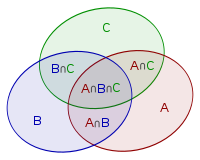
\includegraphics[scale=0.75]{1.png}

Then the area of ​​association $A \cup B \cup C$ equal to the sum of the areas $A$, $B$ and $C$ net twice covered areas $A \cap B$, $A \cap C$, $B \cap C$ But with the addition of three times the area covered $A \cap B \cap C$ :

$S(A\cup B\cup C)=S(A)+S(B)+S(C)-S(A\cap B)-S(A\cap C)-S(B\cap C)+S(A\cap B\cap C)$

Similarly, it can be generalized to the union $n$ figures.

\subsubsection{ Formulation in terms of the probability }

If $A_i$$(I = 1 \ldots n)$ - This event ${\cal P} (A_i)$ - Their probability, then the probability of their union (i.e., what will happen at least one of these events) is:

${\cal P}\left(\bigcup_{i=1}^{n}A_{i}\right)=\sum_{i=1}^{n}{\cal P}(A_{i})-\sum_{1\leq i<j\leq n}{\cal P}(A_{i}\cap A_{j})+\ldots+(-1)^{n-1}{\cal P}(A_{1}\cap\ldots\cap A_{n})$

This amount can also be written as a sum over subsets of $B$ Whose elements are events $A_i$ :

${\cal P}\left(\bigcup_{i=1}^{n}A_{i}\right)=\sum_{C\subseteq B}(-1)^{size(C)-1}{\cal P}\left(\bigcap_{e\in C}e\right)$

\subsection{ Proof of the principle of inclusion-exclusion }

To prove convenient to use the mathematical formulation in terms of set theory:

$\left|\bigcup_{i=1}^{n}A_{i}\right|=\sum_{C\subseteq B}(-1)^{size(C)-1}\left|\bigcap_{e\in C}e\right|$

where $B$ Recall - is the set of $A_i$ 's.

We need to prove that every element contained in at least one of the sets $A_i$, Will take into account the formula exactly once. (Note that the other elements that are not contained in one of the $A_i$ In no way can be considered as not in the right side of the formula).

Consider an arbitrary element $x$ Contained in exactly $k \ge 1$ sets $A_i$. We will show that he considered the formula exactly once.

Note that:

in the terms in which $size (C) = 1$, The element $x$ will take into account exactly $k$ times, with a plus;
in the terms in which $size (C) = 2$, The element $x$ take into account the (negative) exactly $C_k ^ 2$ time - because $x$ count only in those terms, which correspond to the two sets of $k$ sets containing $x$ ;
in the terms in which $size (C) = 3$, The element $x$ will take into account exactly $C_k ^ 3$ times, with a plus;
$\ldots$
in the terms in which $size (C) = k$, The element $x$ will take into account exactly $C_k ^ k$ times, with the sign $(-1) ^ {K-1}$ ;
in the terms in which $size (C)> k$, The element $x$ take into account the zero times.
Thus, we need to calculate a sum of binomial coefficients :

$T=C_{k}^{1}-C_{k}^{2}+C_{k}^{3}-\ldots+(-1)^{i-1}\cdot C_{k}^{i}+\ldots+(-1)^{k-1}C_{k}^{k}$

The easiest way to calculate this amount, comparing it with the expansion in the binomial expression $(1-x) ^ k$ :

$(1-x)^{k}=C_{k}^{0}-C_{k}^{1}\cdot x+C_{k}^{2}\cdot x^{2}-\ldots+(-1)^{k}C_{k}^{k}\cdot x^{k}$

We see that when $x = 1$ expression $(1-x) ^ k$ is none other than $1 - T$. Consequently, the $T = 1 - (1-1) ^ k = 1$, As required.

\subsection{ Usage in solving problems }

The principle of inclusion-exclusion is difficult to understand without a well-studied examples of its applications.

First, we consider three simple problems "on paper", illustrating the application of the principle, and then consider the more practical problems that are difficult to solve without the use of the principle of inclusion-exclusion.

Of particular note is the problem of "search of ways", since it demonstrates that the principle of inclusion-exclusion can sometimes lead to a polynomial solution, not necessarily exponential.

\subsubsection{ The simple task of permutations }

How many permutations of the numbers from $0$ to $9$ such that the first element is larger $1$, And the last - less $8$ ?

Count the number of "bad" permutations, i.e. those in which the first element $\le 1$ and / or last $\ge 8$.

We denote $X$ the set of permutations in which the first element $\le 1$ And through $Y$ - Whose last element $\ge 8$. Then the amount of "bad" permutations on inclusion-exclusion formula is:

$| X | + | Y | - | X \cap Y |.$

After spending some simple combinatorial calculations, we find that this is equal to:

$2 \cdot 9! + 2 \cdot 9! - 2 \cdot 2 \cdot 8!$

Subtracting this number from the total number of permutations $10!$, We get a response.

\subsubsection{ The simple task of (0,1,2)-sequences }

How many sequences of length $n$ Consisting only of numbers $0,1,2$, Each number appears at least once?

Again turn to the inverse problem, i.e., we assume that the number of sequences in which there is not at least one of the numbers.

We denote $A_i$($i = 0 \ldots 2$)The set of sequences in which the number is not found $i$. Then by the inclusion-exclusion number of "bad" sequence is:

$temp$

The dimensions of each of the $A_i$ are obviously $2 ^ n$ (Because such sequences can meet only two digits). Capacity of each pairwise intersection $A_i \cap A_j$ equal $1$ (Still available as only one digit). Finally, the cardinality of the intersection of all three sets is $0$ (Because the available figures do not remain).

Remembering that we solve the inverse problem, we get the final \textbf{answer:}

$3 ^ n - 3 \cdot 2 ^ n + 3 \cdot 1 - 0.$

\subsubsection{ Number of integer solutions of a equation }

Given the equation:

$x_1 + x_2 + x_3 + x_4 + x_5 + x_6 = 20,$

where all $0 \le x_i \le 8$ (Where $i = 1 \ldots 6$ ).

Need to count the number of solutions.

Forget about the first limitation $x_i \le 8$ And simply count the number of non-negative solutions of the equation. This is easily done through the binomial coefficients - we want to break $20$ elements on $6$ groups, i.e., distribute $5$ "Walls" that separate groups, $25$ places:

$N_0 = C_ {25} ^ 5$

Now count on inclusion-exclusion formula number of "bad" decisions, i.e. such solutions, in which one or more $x_i$ more $9$.

We denote $A_k$ (Where $k = 1 \ldots 6$)The set of solutions in which $x_k \ge 9$ And all other $x_i \ge 0$ (For all $i \ne k$ ). To calculate the size of the set $A_k$, We note that we have essentially the same combinatorial problem that was solved in two paragraphs above, but now $9$ items excluded from consideration and exactly belong to the first group. Thus:

$| A_k | = C_ {16} ^ 5$

Similarly, the cardinality of the intersection of two sets $A_k$ and $A_p$ equal to the number:

$\left | A_k \cap A_p \right | = C_7 ^ 5$

The capacity of each intersection of three or more sets is zero, since $20$ elements is not enough for three or more variables, greater than or equal $9$.

Combining all this inclusion-exclusion formula and given that we solve the inverse problem, we finally get \textbf{the answer:}

$C_{25}^{5}-C_{6}^{1}\cdot C_{16}^{5}+C_{6}^{2}\cdot C_{7}^{5}$

\subsubsection{ Number of prime numbers in a given interval }

Let numbers $n$ and $r$. Need to count the number of numbers in the interval $[1; r]$ Prime to $n$.

Go straight to the inverse problem - do not count the number of prime numbers.

Consider all the prime divisors of $n$ And denote them by $p_i$($i = 1 \ldots k$ ).

How many numbers in the interval $[1; r]$ Divisible by $p_i$ ? Their number is:

$\left \lfloor \frac {r} {p_i} \right \rfloor$

However, if we simply sum up these numbers, we get the wrong answer - some numbers to be added together several times (the ones that are divided to several $p_i$ ). Therefore, we must use the inclusion-exclusion formula.

For example, it is possible for $2 ^ k$ enumerate a subset of all $p_i$ 's, Find them work, and to add or subtract to the inclusion-exclusion formula next term.

The final \textbf{implementation} for counting the number of prime numbers:

\begin{verbatim}
int solve(int n, int r){
    vector < int > p ;
    for(int i = 2 ; i * i <= n ; ++ i )
        if(n % i == 0){
            p. push_back(i);
            while(n % i == 0 )
                n / = i ;
        }
    if(n > 1 )
        p. push_back(n);
 
    int sum = 0 ;
    for(int msk = 1 ; msk <(1 << p. size()); ++ msk){
        int mult = 1,
            bits = 0 ;
        for(int i = 0 ; i <(int)p. size() ; ++ i )
            if(msk &(1 << i)) {
                ++ bits ;
                mult * = p[i];
            }
 
        int cur = r / mult ;
        if(bits % 2 == 1 )
            sum + = cur ;
        else
            sum - = cur ;
    }
 
    return r - sum ;
} 
\end{verbatim}
Asymptotics of solutions $O (\sqrt {n})$.

\subsubsection{ Number of integers in a interval, multiple of at least one of the given numbers }

Dana $n$ numbers $a_i$ and the number of $r$. Need to count the number of numbers in the interval $[1; r]$ That are multiples of at least one of $a_i$.

Solution algorithm is almost identical to the previous problem - making inclusion-exclusion formula on numbers $a_i$ Ie Each term in this equation - the number of integers divisible by a given subset of the numbers $a_i$ (That is divisible by their least common multiple ).

Thus, the solution is to ensure that for $2 ^ n$ go through a subset of numbers, for $O (n \log r)$ operations to find their least common multiple, and add or subtract from the response of the next value.

\subsubsection{ Number of strings that satisfy a number of patterns }

Given $n$ patterns - lines of equal length, consisting only of letters and question marks. Also, given the number $k$. Need to count the number of rows that match exactly $k$ patterns or, in other productions, at least $k$ patterns.

First note that we can \textbf{easily count the number of rows that} meet all of the right patterns. You simply "cross" these patterns: a look at the first character (whether in all the patterns in the first position, the question is whether or not at all - if the first character is uniquely defined), the second character, etc.

Now learn how to solve \textbf{the first version of the problem:} when the search strings must satisfy exactly $k$ patterns.

To iterate through this and zafksiruem specific subset $X$ Pattern size $k$ - Now we have to count the number of rows that satisfy this set of patterns and only him. For this we use the inclusion-exclusion formula: we sum over all sets Superset $X$ And either added to the current account, or subtract from it the number of rows that meet the current set:

$ans(X)=\sum_{Y\supseteq X}(-1)^{|Y|-k}\cdot f(Y)$

where $f (Y)$ is the number of rows that meet a set of patterns $Y$.

If we sum $ans (X)$ all $X$, We get the answer:

$ans = \sum_ {X ~: ~ | X | = k} ans (X).$

However, by doing so we got the solution for a time of order $O (3 ^ k \cdot k)$.

The solution can be enhanced by noting that different $ans (X)$ summation is often on the same sets $Y$.

Turn the inclusion-exclusion formula and will lead to the summation $Y$. Then it is easy to understand that many $Y$ will take into account in $C_ {| Y |} ^ k$ inclusion-exclusion formula, always with the same sign $(-1) ^ {| Y |-k}$ :

$ans=\sum_{Y:|Y|\ge k}(-1)^{|Y|-k}\cdot C_{|Y|}^{k}\cdot f(Y)$

Solution has the asymptotics $O (2 ^ k \cdot k)$.

We turn now to the \textbf{second version of the problem:} when the desired lines must meet at least $k$ patterns.

Clearly, we can simply use the solution of the first version of the problem and summarize the responses from $k$ to $n$. However, you can see that all the arguments will still hold, but in this version of the problem by the sum $X$ Not only for those sets whose size is equal to $k$ And for all sets with size $\ge k$.

Thus, in the final formula to $f (Y)$ will be another factor: not one binomial coefficient with some familiar, and their sum:

$(-1)^{|Y|-k}\cdot C_{|Y|}^{k}+(-1)^{|Y|-k-1}\cdot C_{|Y|}^{k+1}+(-1)^{|Y|-k-2}\cdot C_{|Y|}^{k+2}+\ldots+(-1)^{|Y|-|Y|}\cdot C_{|Y|}^{|Y|}$

If you look in Graham(Graham, Knuth, Patashnik. \textbf{"Concrete Mathematics"} [1998] ), we see the well-known formula for the binomial coefficients :

$\sum_{k=0}^{m}(-1)^{k}\cdot C_{n}^{k}=(-1)^{m}\cdot C_{n-1}^{m}$

Applying it here, we see that the whole sum of the binomial coefficients is minimized in:

$(-1) ^ {| Y |-k} \cdot C_ {| Y | -1} ^ {| Y |-k}.$

Thus, for this version of the problem, we also got the solution with the asymptotics $O (2 ^ k \cdot k)$ :

$ans=\sum_{Y:|Y|\ge k}(-1)^{|Y|-k}\cdot C_{|Y|-1}^{|Y|-k}\cdot f(Y)$

\subsubsection{ Number of paths }

There is a field $n \times m$ Some $k$ cells which - impassable wall. On the field, in a cage $(1,1)$ (Lower left cell) is initially robot. The robot can move only right or up and in the end he has to enter the cell $(n, m)$ And avoid all obstacles. Need to count the number of ways in which he can do it.

We assume that the size $n$ and $m$ very large (say, $10 ^ 9$)And the number $k$ - Small (of the order $100$ ).

For solutions at a convenience \textbf{sort} obstacles in the order in which we can avoid them: that is, for example, the coordinate $x$, And at equality - coordinate $y$.

Also, learn how to solve the problem immediately without obstacles: i.e. learn how to count the number of ways to get from one cell to another. If one coordinate we have to go $x$ cells, and on the other - $y$ cells, from a simple combinatorics we get a formula by the binomial coefficients :

$C_ {x + y} ^ {x}$

Now, to count the number of ways to get from one cell to another, avoiding all obstacles, you can use the \textbf{inclusion-exclusion formula:} count the number of ways of walking, stepping at least one obstacle.

This can, for example, go through a subset of the obstacles that we just attack, count the number of ways to do this (just multiplying the number of ways to get from the start to the first cell of the selected constraints of the first obstacles to the second, and so on), and then add or subtract the number of the answer, according to the standard formula of inclusion-exclusion.

However, it will again be nonpolynomial solution - for the asymptotic $O (2 ^ k k)$. We show how to obtain a \textbf{polynomial solution.}

Will solve \textbf{dynamic programming:} learn how to calculate the number of $d [i][j]$ - The number of ways to get $i$ The second point to $j$ Oh, without stepping in it for a single obstacle (except the $i$ and $j$, Of course). All we have $k +2$ point, since the obstacles are added to the start and end cells.

If we for a moment forget about all the obstacles and simply count the number of paths from the cell $i$ squared $j$, We thus take into account some of the "bad" routes through the obstacle. Let us learn to count the number of these "bad" ways. Climb the first obstacle $i <t <j$ To which we attack, then the number of paths is equal to $d [i][t]$ Multiplied by the number of arbitrary ways of $t$ in $j$. Summing it all $t$ We count the number of "bad" ways.

Thus, the value $d [i][j]$ we learned to count the time $O (k)$. Consequently, the solution of the whole problem has asymptotics $O (k ^ 3)$.

\subsubsection{ The number of relatively prime fours }

Given $n$ numbers: $a_1, a_2, \ldots, a_n$. Need to count the number of ways to select four of these numbers so that their combined greatest common divisor is one.

We solve the inverse problem - to count the number of "bad" four, i.e. these quads in which all numbers are divided by the number $d> 1$.

We use the inclusion-exclusion formula, summing the number of fours that are divisible by the divisor $d$ (But perhaps a larger fissile and divider):

$ans = \sum_ {d \ge 2} (-1) ^ {deg (d) -1} \cdot f (d),$

where $deg (d)$ - Is the number of primes in the factorization of $d$, $f (d)$ - The number of fours that are divisible by $d$.

To calculate the function $f (d)$, You simply count the number of multiples $d$ And binomial coefficients count the number of ways to select four of them.

Thus, with the aid of inclusion-exclusion, we summarize the number of fours that are divisible by prime numbers, then subtract the number of fours, dividing by the product of two primes, we add four, divided into three simple, etc.

\subsubsection{ Number of harmonic triplets }

Given the number $n \le 10 ^ 6$. Need to count the number of triples $2 \le a <b <c \le n$ That they are harmonic triplets, i.e.:

or ${\rm gcd} (a, b) = {\rm gcd} (a, c) = {\rm gcd} (b, c) = 1$,
or ${\rm gcd} (a, b)> 1$, ${\rm gcd} (a, c)> 1$, ${\rm gcd} (b, c)> 1$.
First, go straight to the inverse problem - that is, Count the number of non-harmonic triples.

Second, we note that any non-harmonic triple exactly two of its numbers are in this situation, that this number is prime to a number of three and not prime to another number three.

Thus, the amount equal to the sum of non-harmonic triplets over all numbers of $2$ to $n$ products of prime numbers with the current numbers on the number of non-prime numbers.

Now all that's left to solve the problem - is to learn to count every number in the interval $[2; n]$ many numbers are relatively prime (or prime) with him. Although this problem has already been discussed by us above, the solution described above is not appropriate here - it requires factorization of each of the numbers $2$ to $n$ And then iterate through all possible products of prime numbers in the factorization.

Therefore, we need a quick solution that calculates the answers to all numbers in the interval $[2; n]$ immediately.

To do this, you can implement a \textbf{modification of the sieve of Eratosthenes:}

First, we need to find all the numbers in the interval $[2; n]$, In which no prime factorization is not included twice. In addition, for the inclusion-exclusion formula, we need to know how many contain simple factorization of each such number.
To do this, we need to make arrays $deg []$ That hold for any number of simple in its factorization, and $good []$ - Containing every number $true$ or $false$ - All simple enter it in the degree of $\le 1$ or not.

After that, during the processing of the sieve of Eratosthenes next prime number, we'll go over all the multiple of the current number, and increase $deg []$ from them, and all multiples of the square of the current simple - put $good = false$.

Second, we need to find an answer for all the numbers from $2$ to $n$ Ie array $cnt []$ - The number of numbers that are not prime to the data.
For this, we recall how the inclusion-exclusion formula - here we actually implement it the same, but with an inverted logic: if we sort out the term and look at what inclusion-exclusion formula for any numbers, this term is included.

Thus, suppose that we have a number $i$ For which $good [] = true$ Ie the number participating in the inclusion-exclusion formula. Iterate through all the multiples $i$, And the answer $cnt []$ Each of these numbers, we have to add or subtract the value of $\lfloor N / i \rfloor$. Sign - the addition or subtraction - depends on $deg [i]$ : If $deg [i]$ odd, then we must add, or subtract.

\textbf{Implementation:}

\begin{verbatim}
int n ;
bool good[MAXN];
int deg[MAXN], cnt[MAXN];
 
long long solve() {
    memset(good, 1, sizeof good);
    memset(deg, 0, sizeof deg);
    memset(cnt, 0, sizeof cnt);
 
    long long ans_bad = 0 ;
    for(int i = 2 ; i <= n ; ++ i){
        if(good[i ]){
            if(deg[i]== 0) deg[i]= 1 ;
            for(int j = 1 ; i * j <= n ; ++ j){
                if(j > 1 && deg[i]== 1 )
                    if(j % i == 0 )
                        good[i * j]= false ;
                    else
                        ++ deg[i * j];
                cnt[i * j]+ =(n / i)*(deg[i]% 2 == 1 ? + 1 : - 1);
            }
        }
        ans_bad + =(cnt[i]- 1)* 1ll *(n - 1 - cnt[i ]);
    }
 
    return(n - 1)* 1ll *(n - 2)*(n - 3)/ 6 - ans_bad / 2 ;
} 
\end{verbatim}
Asymptotics of the solutions is $O (n \log n)$ Because almost every number $i$ it makes about $n / i$ iterations of inner loop.

\subsubsection{ Number of permutations with no fixed points }

We prove that the number of permutations of length $n$ without fixed points is the next number:

$n!-C_{n}^{1}\cdot(n-1)!+C_{n}^{2}\cdot(n-2)!-\ldots\pm C_{n}^{n}(n-n)!$

and about equal to the number:

$\frac {n! } {E}$

(In fact, if this expression is rounded to the nearest integer - you get exactly the number of permutations with no fixed points)

We denote $A_k$ many permutations of length $n$ with a fixed point in position $k$($1 \le k \le n$ ).

We now use the inclusion-exclusion formula to calculate the number of permutations with at least one fixed point. To do this, we need to learn to consider the size of the sets-intersections $A_i$ They are as follows:

$\left | A_p \right | = (n-1)! ~$

$\left | A_p \cap A_q \right | = (n-2)! ~$

$\left | A_p \cap A_q \cap A_r \right | = (n-3)! ~$

$\ldots ~,$

because if we know that the number of fixed points is $x$, By the same token, we know the position of $x$ elements of the permutation, and the rest $(n-x)$ elements can be anywhere.

Substituting this in inclusion-exclusion, and given that the number of ways to select a subset of size $x$ of $n$ -Element set equal $C_n ^ x$, A formula for the number of permutations with at least one fixed point:

$C_{n}^{1}\cdot(n-1)!-C_{n}^{2}\cdot(n-2)!+\ldots\pm C_{n}^{n}(n-n)!$

Then the number of permutations with no fixed points is:

$n!-C_{n}^{1}\cdot(n-1)!+C_{n}^{2}\cdot(n-2)!-\ldots\pm C_{n}^{n}(n-n)!$

Simplifying this expression, we obtain \textbf{the exact and approximate expressions for the number of permutations with no fixed points:}

$n!\left(1-\frac{1}{1!}+\frac{1}{2!}-\ldots\pm\frac{1}{n!}\right)\approx\frac{n!}{e}$

(Since the sum in brackets - this is the first $n +1$ Members of the Taylor expansion $e ^ {-1}$ )

In conclusion, it is worth noting that a similar problem is solved when you want to fixed points not among $m$ the first elements of the permutation (and not to all, as we have just decided). Will result in the formula as the above exact formula, but it will go up to the sum of $k$ And not to $n$.

\subsection{ Tasks in the online judges }

List of tasks that can be solved by using the principle of inclusion-exclusion:

\begin{itemize}
\item UVA 10325 \textbf{"The Lottery"} [Difficulty: Easy]

\item UVA 11806 \textbf{"Cheerleaders"} [Difficulty: Easy]

\item TopCoder SRM 477 \textbf{"CarelessSecretary"} [Difficulty: Easy]

\item TopCoder TCHS 16 \textbf{"Divisibility"} [Difficulty: Easy]

\item SPOJ 6285 NGM2 \textbf{"Another Game With Numbers"} [Difficulty: Easy]

\item TopCoder SRM 382 \textbf{"CharmingTicketsEasy"} [Difficulty: Medium]

\item TopCoder SRM 390 \textbf{"SetOfPatterns"} [Difficulty: Medium]

\item TopCoder SRM 176 \textbf{"Deranged"} [Difficulty: Medium]

\item TopCoder SRM 457 \textbf{"TheHexagonsDivOne"} [Difficulty: Medium]

\item SPOJ 4191 MSKYCODE \textbf{"Sky Code"} [Difficulty: Medium]

\item SPOJ 4168 SQFREE \textbf{"Square-free integers"} [Difficulty: Medium]

\item CodeChef \textbf{"Count Relations"} [Difficulty: Medium]
\end{itemize}

\subsection{ Literature }

Debra K. Borkovitz. \textbf{"Derangements and the Inclusion-Exclusion Principle"}

\section{ Games on arbitrary graphs }
Let the game is played by two players on some graph G. Ie current state of the game - is a vertex of the graph, and each of the vertices of the edge going into the vertices, which can go on the next move.

We consider the most general case - the case of an arbitrary directed graph with cycles. Required for a given initial position to determine who will benefit from the best game of both players (or determine that the result is a draw).

We will solve this problem very effectively - find answers to all the vertices in linear time on the number of edges - \textbf{O (M).}

\subsection{ Description of the algorithm }
About some of the vertices of the graph is known in advance that they are winning or as lost, obviously, such peaks have outgoing edges.

We have the following \textbf{facts:}

If a vertex of an edge in a losing vertex, then this vertex is winning;
If a vertex of all the edges come in winning the top, then this vertex is losing;
if at any time there are still undefined peak, but none of them do not fit under the first or under the second rule, all of these peaks - draw.
Thus, the algorithm is clear, working for the asymptotic behavior of O (NM) - we iterate through all the vertices, each trying to use the first or the second rule, and if we have made some changes, then repeat again.

However, the process of finding and updating can be sped up, increasing to the asymptotic linear.

Iterate through all the vertices of which are originally known to be winning or losing. From each of them let the next search in depth. This depth-first search will move in the opposite edges. First of all, it will not come to the top, which is defined as winning or losing. Further, if the DFS tries to go to the top of losing a vertex, then it is marked as a winning, and goes to her. If DFS tries to go out a winner in the top of a vertex, it must check that all the ribs are out of this top in winning. This test is easy to implement for the O (1) if each node will store counter edges that lead to winning the top. So, if the DFS tries to go out a winner in the top of a vertex, then it increases to counter it, and if the counter is equal to the number of edges emanating from the vertex, then this vertex is marked as losing, and depth-first search is the vertex. Otherwise, if the target vertex and is not defined as a winning or losing, the depth-first search does not come into it.

Total, we see that each and every winning losing vertex visited our algorithm only once, and no man's peaks and did not attend. Consequently, the asymptotic really \textbf{O (M).}

\subsection{ Implementation }
Consider the implementation of depth-first search, on the assumption that the graph is built in the memory of the game, the outcome of the degree are counted and recorded in degree (this is just a counter, it will be reduced if there is an edge in winning the top), and the original winning or losing is tops labeled.

\begin{verbatim}
 vector <int> g [100];
 bool win [100];
 bool loose [100];
 bool used [100];
 int degree [100];

 void dfs (int v) {
     used [v] = true;
     for (vector <int>::iterator i = g [v]. begin(); i! = g [v]. end();++ i)
         if (! used [* i]) {
             if (loose [v])
                 win [* i] = true;
             else if (- degree [* i] == 0)
                 loose [* i] = true;
             else
                 continue;
             dfs (* i);
         }
 } 
\end{verbatim}\subsection{ An example of a problem: "Police and Thief" }
Algorithm to become more clear, we consider it a concrete example.

\textbf{Condition of the problem.} There is a field size MxN cells, some cells can not go. Known coordinates of the origin of police and thief. Also on the card may be present output. If the police will be in the same cage with the thief, the police won. If the thief be in the cell with the output (in this cell should not police), you will win a thief. A police officer can walk in 8 directions, the thief - only 4 (along the axes). And the police, and the thief may pass their turn. The first course of a police officer does.

\textbf{Graphing.} A graph game. We need to formalize the rules of the game. The current state of the game is determined by the coordinates of police P, Thief T, as well as boolean Pstep, which determines who will make the next move. Consequently, the vertex of the graph is defined by the triple (P, T, Pstep). Count to build easy, simple matching condition.

Next you need to determine which vertices are won or as lost initially. There is a \textbf{subtle point.} Winning / Losing top addition to the coordinates depends on Pstep - whose turn. If you now move the police, then the top of winning, if the coordinates of a policeman and the thief are the same, apex lost if it is not winning and the thief is on the way out. If we now move the thief, then the top of winning, if the thief is on the way out and losing, if it is not advantageous and coordinate police and thief are the same.

The only time you want to solve - build \textbf{graph clearly or} do it \textbf{"on the fly",} right in the DFS. On the one hand, if we construct a graph in advance, it will be less likely to make mistakes. On the other hand, it will increase the amount of code, and the work will be several times slower than if you build the graph "on the go."

\textbf{The implementation} of the program:

\begin{verbatim}
 struct state {
     char p, t;
     bool pstep;
 };

 vector <state> g [100][100][2];
 // 1 = policeman coords; 2 = thief coords; 3 = 1 if policeman's step or 0 if thief's.
 bool win [100][100][2];
 bool loose [100][100][2];
 bool used [100][100][2];
 int degree [100][100][2];

 void dfs (char p, char t, bool pstep) {
     used [p][t][pstep] = true;
     for (vector <state>::iterator i = g[p][t][pstep].begin(); i! = g[p][t][pstep]. end();++ i)
         if (! used [i-> p][i-> t][i-> pstep]) {
             if (loose [p][t][pstep])
                 win [i-> p][i-> t][i-> pstep] = true;
             else if (- degree [i-> p][i-> t][i-> pstep] == 0)
                 loose [i-> p][i-> t][i-> pstep] = true;
             else
                 continue;
             dfs (i-> p, i-> t, i-> pstep);
         }
 }


 int main() {

     int n, m;
     cin >> n >> m;
     vector <string> a (n);
     for (int i = 0; i <n;++ i)
         cin >> a [i];

     for (int p = 0; p <n * m;++ p)
         for (int t = 0; t <n * m;++ t)
             for (char pstep = 0; pstep <= 1;++ pstep) {
                 int px = p / m, py = p% m, tx = t / m, ty = t% m;
                 if (a [px][py] == '*' | | a [tx][ty] == '*') continue;
                
                 bool & wwin = win [p][t][pstep];
                 bool & lloose = loose [p][t][pstep];
                 if (pstep)
                     wwin = px == tx && py == ty, lloose =! wwin && a [tx][ty] == 'E';
                 else
                     wwin = a [tx][ty] == 'E', lloose =! wwin && px == tx && py == ty;
                 if (wwin | | lloose) continue;

                 state st = {p, t,! pstep};
                 g [p][t][pstep]. push_back (st);
                 st.pstep = pstep! = 0;
                 degree [p][t][pstep] = 1;
                
                 const int dx [] = {-1, 0, 1, 0, -1, -1, 1, 1};
                 const int dy [] = {0, 1, 0, -1, -1, 1, -1, 1};
                 for (int d = 0; d <(pstep? 8:4);++ d) {
                     int ppx = px, ppy = py, ttx = tx, tty = ty;
                     if (pstep)
                         ppx + = dx [d], ppy + = dy [d];
                     else
                         ttx + = dx [d], tty + = dy [d];
                     if (ppx>= 0 && ppx <n && ppy>= 0 && ppy <m && a [ppx][ppy]! = '*' &&
                         ttx>= 0 && ttx <n && tty>= 0 && tty <m && a [ttx][tty]! = '*')
                     {
                         g [ppx * m + ppy][ttx * m + tty][! pstep]. push_back (st);
                        ++ Degree [p][t][pstep];
                     }
                 }
             }

     for (int p = 0; p <n * m;++ p)
         for (int t = 0; t <n * m;++ t)
             for (char pstep = 0; pstep <= 1;++ pstep)
                 if ((win [p][t][pstep] || loose[p][t][pstep]) && !used[p][t][pstep])
                     dfs (p, t, pstep! = 0);

     int p_st, t_st;
     for (int i = 0; i <n;++ i)
         for (int j = 0; j <m;++ j)
             if (a [i][j] == 'C')
                 p_st = i * m + j;
             else if (a [i][j] == 'T')
                 t_st = i * m + j;

     cout << (win [p_st][t_st][true]? "WIN": loose[p_st][t_st][true]? "LOSS": "DRAW");

 } 
\end{verbatim}

\section{ Sprague-Grundy theory for games }
\subsection{ Introduction }

Theory Sprague Grundy - a theory that describes the so-called \textbf{equal} (born "impartial") play two players, i.e. games, which allowed the moves and the winning / losing one depends only on the state of the game. On which of the two players go, nothing is independent: i.e. players are completely equal.

In addition, it is assumed that the players have all the information (about the rules of the game, the possible moves, standing opponent).

It is assumed that the game is \textbf{finite,} that is for any strategy players will sooner or later come to \textbf{a losing} position from which there is no transition to other positions. This position is a loser for the player who has to make a move from this position. Accordingly, it is advantageous for a player who came into this position. Clearly, a draw in a game does not happen.

In other words, this game can be completely described \textbf{a directed acyclic graph:} vertices there are state of the game, and the ribs - transitions from one state to another game as a result of the current player's turn (again, in the first and second player are equivalent). One or more nodes have no outgoing edges, it is as lost vertices (for a player who has to make a move from the top).

Since a tie does not happen, then all the states of the game are divided into two classes: \textbf{the winning and losing.} Winning - these are states that there is a move the current player, which will lead to inevitable defeat another player even during his best game. Accordingly, losing the state - a state from which all transitions lead to states, leading to the victory of the second player, in spite of the "resistance," the first player. In other words, the winner will state from which there is at least one transition in a losing state, and losing a state from which all transitions lead to winning the state (or from which there are no transitions).

Our task - for any given game to classify the states of the game, that is, for each state to determine the winning or losing it.

The theory of games independently developed Roland Sprague in 1935 and Patrick Michael Grundy in 1939

\subsection{ Nim game }

This game is one of the examples described above games. Moreover, as we shall see \textbf{later,} each of equal game two players are actually equivalent to the game "them" (English "nim"), so the study of the game will allow us to automatically solve all the rest of the game (but more on that later).

Historically, this game was popular in ancient times. Probably the game has its origins in China - at least, the Chinese game "Jianshizi" is very similar to him. In Europe, the first mention of Nimes are in the XVI. The name "it" invented mathematician Charles Bud (Charles Bouton), which in 1901 published a full analysis of the game. The origin of the name "it" is not known.

\subsubsection{ Game description }

Game "it" is a next game.

There are several piles, each with a few stones. In one move, the player can take any one of a handful of any non-zero number of stones and throw them away. Accordingly, the loss occurs when there are no more moves, i.e. All piles are empty.

So, the state of the game "them" uniquely describes an unordered set of natural numbers. In one move allowed strictly to reduce any of the numbers (if the resulting number will be zero, it is removed from the set.)

\subsubsection{ Solution of nim }

The solution of this game published in 1901 by Charles Bud (Charles L. Bouton), and it looks as follows.

\textbf{Theorem.} Current player has a winning strategy if and only if the XOR-sum of the sizes of heaps is nonzero. Otherwise, the current player is in a losing position. (XOR-sum of the numbers $a_i$ is an expression $a_1 \oplus a_2 \oplus \ldots \oplus a_n$ Where $\oplus$ - Bitwise exclusive or)

\textbf{Proof.}

The main essence of the proof below - in the presence of \textbf{symmetric strategies for the opponent.} We show that, being in a state of zero XOR-sum, the player will not be able to get out of this state - in any of its transition to a state with nonzero XOR-sum of the enemy there is a retaliatory move that returns the XOR-sum back to zero.

We now turn to the formal proof (it will be constructive, that's how it looks balanced strategy of the enemy - which one will have to move him to perform).

Will prove the theorem by induction.

For an empty neem (when the size of all the heaps are zero) XOR-sum is zero, and the theorem is true.

Now suppose that we want to prove the theorem for a state of the game, from which there is at least one transition. Using the induction hypothesis (and acyclic games), we believe that the theorem is true for all the states in which we can get from this.

Then the proof is divided into two parts: if the XOR-sum $s$ in the current state $= 0$ It is necessary to prove that the current state is losing, i.e. all transitions from it lead to states with XOR-sum $t \ne 0$. If the $s \ne 0$ It is necessary to prove that there is a transition that leads us to a state of $t = 0$.

Let $s = 0$, Then we want to show that the current state - losing. Consider any transition from the current state of neem: we denote $p$ Rooms vary a bunch through $x_i$($i = 1 \ldots n$)- The size of piles to travel through $y_i$($i = 1 \ldots n$)- After the move. Then, using the elementary properties of the function $\oplus$, We have:
$t=s\oplus x_{p}\oplus y_{p}=0\oplus x_{p}\oplus y_{p}=x_{p}\oplus y_{p}$

But since $y_p <x_p$, This means that $t \ne 0$. Hence, the new state will be non-zero XOR-sum, that is, according to the basis of the induction will be advantageous, as required.

Let $s \ne 0$. Then our task - to prove that the current state - winning, i.e. of course it exists in a losing state (zero-XOR-sum).
Consider a bit of a record $s$. Take the highest non-zero bit, let his number is $d$. Let $k$ - The number of the pile, the size $x_k$ which $d$ First bit different from zero (such $k$ there, otherwise it would amount to the XOR- $s$ this bit would not have been different from zero.)

If approved, the required course - is to change $k$ Th pile, making it the size of the $y_k = x_k \oplus s$.

Let us prove this.

First you have to check that this is the correct move, i.e. that $y_k <x_k$. But that is because all of the bits, the senior $d$ The second, the $x_k$ and $y_k$ the same, and in $d$ Th bit in $y_k$ will be zero, while the $x_k$ will be one.

Now calculate what XOR-sum obtained with the course:

$t=s\oplus x_{k}\oplus y_{k}=s\oplus x_{k}\oplus(s\oplus x_{k})=0$

Thus, this move us - really move in a losing state, and this proves that the current state winner.

Theorem.

\textbf{Corollary.} Any condition them games can be replaced by an equivalent condition, which consists of only a handful of size equal to the XOR-sum of the sizes of piles in the old state.

In other words, the analysis of neem with several batches can calculate the amount of XOR- $s$ their size, and to the analysis of only a handful of neem size $s$ - As the theorem just proved, the winning / losing one will not change.

\subsection{ Equivalence of any game to nim }

Here, we show how any game (game two equal players) associate him. In other words, any state of any game we will learn to associate the pile-it completely describes the state of the original game.

\subsubsection{ Lemma of nim with increases }

Let us first prove a very important result - \textbf{lemma Nimes with increases.}

Specifically, consider the following modified them all the same way as in the usual Nimes, but now allowed to view additional course: instead of reducing, on the contrary, \textbf{increase the size of a handful.} To be more precise, the player's turn now is that he either takes a non-zero number of stones from any pile, or increase the size of a handful (as with certain rules, see next paragraph).

It is important to understand that the rules of how the player can make larger, \textbf{we do not care} - but these rules still have to be to our game was still \textbf{acyclic.} Below in the section "Examples of games," the examples of these games, "Stair him", "nimble-2", "turning turtles".

Again, we will prove the lemma in general, for any game of this type - games like "him with increases"; specific rules increases in the proof can not be used.

\textbf{Lemma.} It is equivalent to increases nimu normal, in the sense that the winning / losing end state is determined by a theorem according to Bouton XOR-sum of the sizes of heaps. (Or, in other words, the essence of the lemma is that the increase is useless, they do not make sense to apply the optimal strategy, and they do not change a winning / losing end as compared to conventional Nimes.)

\textbf{Proof.}

The idea of the proof, as in Theorem Bouton - Available \textbf{symmetric strategy.} We show that the increase does not change anything, because after one of the players resort to increase, the other will be able to answer it symmetrically.

Indeed, suppose that the current player makes a stroke-increasing piles. Then his opponent could just answer it, reducing it back to the pile of old values ​​- for the usual moves neem we still may be used freely.

Thus, a symmetric response to the stroke-stroke-increase will reduce the size back to the old heap. Therefore, after this answer game comes back to the same size of heaps, i.e. a player who has made an increase, do nothing to win. Because acyclic game, sooner or later run out of moves, increasing, and current players have to make a move, zoom out, and this means that the presence of increasing moves does not change anything.

\subsubsection{ Sprague Grundy theorem on the equivalence of any game to nim }

We now turn to the most important fact in this article - the equivalence theorem nimu any equitable playing two players.

\textbf{Theorem Sprague Grundy.} Consider any state $v$ equal a game of two players. He has let out some of the transitions in the state $v_i$$(I = 1 \ldots k)$ (Where $k \ge 0$ ). State that the $v$ this game can be associated with a handful of neem certain size $x$ (Which will fully describe the state of $v$ our game - that is, these two states are two different games are equivalent.) This number is $x$ - Is called the \textbf{value Sprague Grundy} status $v$.

Moreover, this number $x$ You can find the following recursive way: Calculate the value Sprague Grundy $x_i$ for each transition $(V, v_i)$ And then executed:

$x = {\rm mex} \{x_1, \ldots, x_k \},$

where the function $\rm mex$ of a set of numbers returns the smallest non-negative number is not found in this set (the name "mex" - an abbreviation of "minimum excludant").

Thus, we can, starting from the vertices without outgoing edges, slowly \textbf{count values ​​Sprague Grundy for all the states of the game.} If the value Sprague Grundy any state is zero, then this state is losing, otherwise - winner.

\textbf{Proof.} Will prove the theorem by induction.

For vertices, of which there is no transition, the $x$ Theorem will be obtained as $\rm mex$ the empty set, i.e., $x = 0$. But, in fact, without a transition state - is losing condition, and he really should meet him, a bunch of size $0$.

Consider now any state $v$ Of which there are transitions. By induction, we can assume that for all states $v_i$ In which we can move from the current state, the value $x_i$ already counted.

Calculate the amount of $p = {\rm mex} \{x_1, \ldots, x_k \}$. Then, by the definition of $\rm mex$, We see that for any number $i$ in the interim $[0; p)$ there is at least one corresponding transition into some of $v_i$ 's Condition. In addition, there may be additional transitions - to states with values ​​Grundy, large $p$.

This means that the current state \textbf{equivalent to the state nimu with increases in size with a small group} \textbf{$p$} : In fact, we have a transition from the current state to a state with a bunch of smaller sizes, and can be transitions to states large.

Consequently, the value ${\rm mex} \{x_1, \ldots, x_k \}$ really is the desired value Sprague Grundy for the current status, as required.

\subsection{ Application of Sprague Grundy Theorem  }

Finally we describe the holistic algorithm is applicable to any two-player game equal to determine the winning / losing end of the current state $v$.

Function that each of the game assigns to him a number, called a \textbf{function Sprague Grundy.}

So, to find a function Sprague Grundy for the current state of a game, you need:

List all the possible transitions from the current state.
Each transition can be managed either in a single game, or in \textbf{the amount of independent games.}
In the first case - just count the Grundy function recursively for the new state.

In the second case, when the transition from the current state results in the sum of several independent games - recursively count for each of these games Grundy function, then we say that the function of the amount of games Grundy is XOR-sum of the values ​​of these games.

Once we thought Grundy function for each possible move - believe $\rm mex$ from these values, and found number - is the desired value for the current state of Grundy.
If the value is zero Grundy, the current state of the disadvantageous - otherwise advantageous.
Thus, in comparison with Theorem Sprague Grundy here we take into account the fact that the game can be transitions from the individual states in the \textbf{amount of several games.} To work with the amounts of games, we first replace each game its value Grundy, i.e. a handful of them, of a certain size. After that we come to him, the sum of several piles, i.e. to normal nimu, the answer to which, according to Theorem Bouton - XOR-sum of the sizes of heaps.

\subsection{ Regularities in the ​​Sprague Grundy values  }

Very often for specific tasks when required to learn to count function Sprague Grundy for a given game, helps \textbf{you study the table of} this function in search of patterns.

In many games that seem very difficult for a theoretical analysis, the function Sprague Grundy in practice is periodic, or as having a very simple form that is easy to notice "the eye." In the majority of cases seen by the laws are valid, and if desired, proved using induction.

However, not always function Sprague Grundy contains simple patterns, and for some, even very simple in its formulation, games, whether such laws are still open (for example, "Grundy's game" below.)

\subsection{ Examples of games }

To demonstrate the theory Sprague Grundy, explain a few problems.

Especially it is necessary to draw attention to the problem, "it stair", "nimble-2", "turning turtles", which shows how trivial the original problem to nimu zoom.

\subsubsection{ "Tic-Tic" }

\textbf{Condition.} Consider the size of the plaid stripes $1 \times n$ cells. In one move, the player must put one cross, but it is forbidden to put two crosses near (to neighboring cells). The player who can not make a move. To say who will win the game at the optimum.

\textbf{Decision.} When a player puts a cross in any cell, it can be assumed that the entire band is divided into two separate halves: the left of the cross and to his right. In this case, the cell itself with the cross, and its left and right neighbor destroyed - because they can not be anything else to put.

Consequently, if we number the cells from the strip $1$ to $n$ Then, put a cross in the position $1 <i <n$, Band splits into two long strips $i-2$ and $n-i-1$ Ie We turn to the sum of the two games $i-2$ and $n-i-1$. If the cross is placed in the position $1$ or $n$, This is a special case - we just move on to the state $n-2$.

Thus, the function Grundy $g [n]$ has the form (for $n \ge 3$ )

$g[n]={\rm mex}\left\{ g[n-2],\,\bigcup_{i=2}^{n-1}\left(g[i-2]\oplus g[n-i-1]\right)\right\} $

Ie $g [n]$ obtained as $\rm mex$ from the set consisting of the numbers $g [n-2]$ And the possible values ​​of expressions $g [i-2] \oplus g [n-i-1]$.

So we have this objective $O (n ^ 2)$.

In fact, considering the computer table of values ​​for the first hundred values $n$, You can see that from $n = 52$, The sequence $g [n]$ is periodic with period $34$. This pattern is maintained and further (which probably can be proved by induction).

\subsubsection{ "Noughts and crosses - 2" }

\textbf{Condition.} Again, the game is on the strip $1 \times n$ cells, and the players take turns to put one dagger. The winner is the one who put the three crosses in a row.

\textbf{Decision.} Note that if the $n> 2$ and we left after a stroke two crosses near or over one space, the opponent wins the next move. Consequently, if one player has put a cross somewhere, then another player put a cross in the disadvantageous its neighboring cells, as well as in neighboring adjacent (i.e., at a distance $1$ and $2$ disadvantageous place, it will lead to the defeat).

Then the solution is almost similar to the previous problem, but now the cross is removed from each half of not one, but two cells.

\subsubsection{ "Pawns" }

\textbf{Condition.} There is a field $3 \times n$ In which the first and the third row are for $n$ pawns - white and black, respectively. The first player plays white pawns, the second - black. The turn and strike - standard chess, except that beat (where available) is mandatory.

\textbf{Decision.} Let us see what happens when one pawn will move ahead. Next move, the opponent will be obliged to eat it, then we'll have to eat a pawn of the opponent, then he eats, and, finally, our enemy pawn pawn eat and stay, "resting" in the opponent's pawn. Thus, if we are in the beginning walked in column $1 <i <n$, The result of three columns $[I-1; i +1]$ board virtually annihilated, and we get to the size of the amount of games $i-2$ and $n - i - 1$. Boundary cases $i = 1$ and $i = n$ just bring us up to the board size $n-2$.

Thus, we obtain an expression for the function Grundy, similar to the above problem "Tic-tic."

\subsubsection{ "Lasker's nim" }

\textbf{Condition.} There is $n$ cairns set sizes. In one move, the player can take any non-zero number of stones from a pile, or else split any pile into two nonempty piles. The player who can not make a move.

\textbf{Decision.} Writing both types of transitions easily function Sprague Grundy as:

$g[n]={\rm mex}\left\{ \bigcup_{i=0}^{n-1}g[i],\,\bigcup_{i=1}^{n-1}\left(g[i]\oplus g[n-i]\right)\right\} $

However, you can build a table of values ​​for small $n$ and see a simple rule:

$\begin{array}{ccccccccccccccccccccc}
n & 0 & 1 & 2 & 3 & 4 & 5 & 6 & 7 & 8 & 9 & 10 & 11 & 12 & 13 & 14 & 15 & 16 & 17 & 18 & 19\\
g[n] & 0 & 1 & 2 & 4 & 3 & 5 & 6 & 8 & 7 & 9 & 10 & 12 & 11 & 13 & 14 & 16 & 15 & 17 & 18 & 20
\end{array}$

You can see that $g [n] = n$ for numbers equal $1$ or $2$ modulo $4$ And $g [n] = n \pm 1$ for numbers equal $3$ and $0$ modulo $4$. You can prove this by induction.

\subsubsection{ "The game of Kayles" }

\textbf{Condition.} There is $n$ pins on display in a row. For one kicker can beat either one skittle or two standing next to the pins. The winner is the one who knocked out the last pin.

\textbf{Decision.} And when a player kicks a kingpin, and when he knocks out two - the game is divided into the sum of two independent games.

Easy to obtain an expression for the function Sprague Grundy:

$g[n]={\rm mex}\left\{ \bigcup_{i=0}^{n-1}\left(g[i]\oplus g[n-1-i]\right),\,\bigcup_{i=0}^{n-2}\left(g[i]\oplus g[n-2-i]\right)\right\} $

Count for a table for the first few tens of elements:

$\begin{array}{ccccccccccccc}
g[0\ldots11] & 0 & 1 & 2 & 3 & 1 & 4 & 3 & 2 & 1 & 4 & 2 & 6\\
g[12\ldots23] & 4 & 1 & 2 & 7 & 1 & 4 & 3 & 2 & 1 & 4 & 6 & 7\\
g[24\ldots45] & 4 & 1 & 2 & 8 & 5 & 4 & 7 & 2 & 1 & 8 & 6 & 7\\
g[36\ldots47] & 4 & 1 & 2 & 3 & 1 & 4 & 7 & 2 & 1 & 8 & 2 & 7\\
g[48\ldots59] & 4 & 1 & 2 & 8 & 1 & 4 & 7 & 2 & 1 & 4 & 2 & 7\\
g[60\ldots71] & 4 & 1 & 2 & 8 & 1 & 4 & 7 & 2 & 1 & 8 & 6 & 7\\
g[72\ldots83] & 4 & 1 & 2 & 8 & 1 & 4 & 7 & 2 & 1 & 8 & 2 & 7\\
g[84\ldots95] & 4 & 1 & 2 & 8 & 1 & 4 & 7 & 2 & 1 & 8 & 2 & 7\\
g[96\ldots107] & 4 & 1 & 2 & 8 & 1 & 4 & 7 & 2 & 1 & 8 & 2 & 7\\
g[108\ldots119] & 4 & 1 & 2 & 8 & 1 & 4 & 7 & 2 & 1 & 8 & 2 & 7
\end{array}$

It can be noted that, from a certain moment, the sequence is periodic with period $12$. In the future, this periodicity is also not violated.

\subsubsection{ Grundy's game }

\textbf{Condition.} There is $n$ cairns, the size of which will be denoted by $a_i$. In one move, the player can pick up an order of at least a handful of $3$ and divide it into two nonempty piles of unequal size. The player who can not make a move (i.e., the size of all the remaining piles of less than or equal to two).

\textbf{Decision.} If $n> 1$, Then these few piles obviously - independent games. Therefore, our task - to learn to look for the function Sprague Grundy for a handful, and the answer for a few piles will be obtained as their XOR-sum.

For a handful of this function is constructed as easy enough to see all the possible transitions:

$g[n]={\rm mex}\left\{ \bigcup_{i=[1\ldots n-1],i\ne n-i}\left(g[i]\oplus g[n-i]\right)\right\} $

What this game is interesting - the fact that so far it has been found for the general law. Despite the assumption that the sequence $g [n]$ should be periodic, it was calculated up to $2 ^ {35}$ And periods in this area were found.

\subsubsection{ "Stair him" }

\textbf{Condition.} There are stairs to the $n$ steps (numbered from $1$ to $n$)For $i$ The second step is $a_i$ coins. In one move is allowed to move a non-zero number of coins with $i$ Th at $i-1$ Th step. The player who can not make a move.

\textbf{Decision.} If you try to reduce this problem to nimu "head-on", it turns out that the course we have - is to reduce one heap on how many, and the simultaneous increase in the other pile on as much. The result is a modification of neem, which is very difficult to solve.

Proceed in a different way: we consider only the odd-numbered steps: $a_1, a_3, a_5, \ldots$. Let's see how this will change the set of numbers when making a turn.

If the move is made with an even $i$, Then this move mean more $a_ {i-1}$. If the move is made with the odd $i$, This means a reduction $a_i$.

It turns out that our problem - it is ordinary with increases in the size of heaps $a_1, a_3, a_5, \ldots$.

Therefore, the function Grundy from it - it's XOR-sum of the numbers of the form $a_ {2i +1}$.

\subsubsection{ "Nimble" and "Nimble-2" }

\textbf{Condition.} There is a strip of plaid $1 \times n$ On which the $k$ coins: $i$ Th coin is in $a_i$ Th cell. In one move, the player can take some coin and move it to the left by an arbitrary number of cells, but that it did not come out beyond the strip. In the game "Nimble-2" extra jump prohibited other coins (or even put two coins in one cell). The player who can not make a move.

\textbf{Decision "Nimble".} Note that the coins in this game are independent of each other. Moreover, if we consider a set of numbers $a_i-1$$(I = 1 \ldots k)$, It is clear that one player may take any of these numbers, and reduce it, but a loss is when all the numbers are equal to zero. Consequently, the game "Nimble" - \textbf{it} is the \textbf{usual,} and the answer to the problem is the XOR-sum of the numbers $a_i-1$.

\textbf{Decision "Nimble-2."} We number the coins in the order they appear from left to right. Then we denote $d_i$ distance from $i$ Nd to $i-1$ The second coins:

$d_i = a_i - a_ {i-1} - 1, ~ ~ ~ ~ (i = 1 \ldots k)$

(Assuming that $a_0 = 0$ ).

Then one player can take away from some $d_p$ a number $q$, And add the same number $q$ to $d_ {p +1}$. Thus, this game - it is actually the \textbf{"stair him"} over numbers $d_i$ (We just have to change the order of the numbers on the opposite).

\subsubsection{ "Turning turtles" and "Twins" }

\textbf{Condition.} Dana plaid stripe size $1 \times n$. Each cell is either a cross or crosses. In one move, you can take a toe and turn it into a cross.

While \textbf{additionally} allowed to choose one of the boxes to the left of the variable and change it to the opposite value (i.e. toe to replace the cross, and the cross - the toe). In the game "turning turtles" this is not required (i.e. the player may be limited to the conversion of Os X), and the "twins" - necessarily.

\textbf{Decision "turning turtles".} States that this game - it is a regular on the numbers $b_i$ Where $b_i$ - Position $i$ On O's (1-indexed). Verify this assertion.

If a player is simply reversed toe on the cross, do not use an additional way - it can be understood as the fact that he just took the whole pile, corresponding to that of Os. In other words, if a player changed his toe on a cross in the position $x$$(1 \le x \le n)$, That by doing so he took a bunch of size $x$ and made it a size zero.
If a player took an additional course, that in addition to what has changed in the cross position $x$ to toe, he has changed the cell in position $y$$(Y <x)$, We can assume that he reduced the pile $x$ to the size of $y$. Indeed, if the position $y$ used to be a cross - that, in fact, after the course there will be a player crosses, i.e. will pile size $y$. And if in the position of $y$ used to be a toe, then after playing a handful of players this disappears - or, equivalently, a second handful of exactly the same size $y$ (As in Nimes two piles of the same size actually "kill" each other).
Thus, the answer to the problem - it is XOR-sum of the numbers - the coordinates of all the zeroes in the 1-indexed.

\textbf{Decision "twins".} All the above arguments are still valid, except that the move "pile reset" is now the player does not. Ie If we subtract the coordinates of all the unit - the game will turn back to normal it.

Thus, the answer to the problem - it is XOR-sum of the numbers - the coordinates of all the zeroes in the 0-indexed.

\subsubsection{ Northcott's game }

\textbf{Condition.} A board size $n \times m$ : $n$ rows and $m$ columns. In each row there are two chips: one black and one white. In one move, the player can take any piece of the same color, and move it inside the line to the right or to the left by an arbitrary number of steps, but not jumping over another piece (and not getting it). The player who can not make a move.

\textbf{Decision.} First, it is clear that each of the $n$ lines form an independent board game. Therefore, the task is to analyze the game in a row, and the answer to the problem will be the sum of the XOR-Sprague Grundy for each one.

Solving the problem for a single line, let $x$ the distance between the black and white pieces (which can vary from zero to $m-2$ ). In one turn, each player may either reduce $x$ for some arbitrary value, or possibly increase it to some value (larger is not always available). Thus, this game - it is \textbf{"them with increases",} and, as we already know, the increase in this game is useless. Therefore, the function Grundy for one line - this is the distance $x$.

(Note that formally this argument is incomplete - as in "with increases in Nimes" assumes that the game \textbf{is finite,} and here the game allow players to play indefinitely. However, endless game can not take place at an optimal game - that because one player is to increase the distance $x$ (The price closer to the edge of the field), the other player close to him, reducing $x$ back. Consequently, for optimal game opponent player will not be able to make the moves increase indefinitely, so still described the solution remains in effect.)

\subsubsection{ Triomino }

\textbf{Condition.} Given the size of the field of cellular $2 \times n$. In one move, a player can bet on the one figure in the shape of the letter "G" (i.e., a coherent shape from the three cells that do not lie on the same line). It is forbidden to put a figure so that it crossed at least one cell with one of the figures that have been set. The player who can not make a move.

\textbf{Decision.} Note that the formulation of a figure partitions the field into two separate fields. Thus, we have to analyze not only the rectangular field, but the field in which the left and / or right edges are uneven.

Drawing a different configuration, you can see that no matter what the configuration of the field, the main thing - just how many cells on the field. In fact, if the current field $x$ free cells, and we want to break this field into two fields the size of $y$ and $z$ (Where $y + z +3 = x$ ), It is always possible that you can always find an appropriate place for figures.

Thus, our task becomes this: initially, we have a bunch of stones the size of $2n$ And in one move we can throw out a bunch of $3$ stone and then smash the pile into two piles of arbitrary size. Grundy function for this game is:

$g[n]={\rm mex}\left\{ \bigcup_{i=0}^{n-3}\left(g[i]\oplus g[n-i-3]\right)\right\} $

\subsubsection{ Chips on a graph }

\textbf{Condition.} Given a directed acyclic graph. In some of the vertices of the graph are the chips. In one move, the player can take any piece and move it along any edge in the new vertex. The player who can not make a move.

Also happens to be the second version of this problem, when it is considered that if the two pieces come in one vertex, then they both cancel each other out.

\textbf{Decision of the first variant of the problem.} First, all the chips - are independent of each other, so our task - to learn how to look for a Grundy function for one chip in the graph.

Given that the graph is acyclic, we can do it recursively: Assume that we thought Grundy function for all the children of the current node. Then the function Grundy in the current top - it $\rm mex$ from this set of numbers.

Thus, the solution of the problem is the following: for each vertex recursively find Grundy function, if it was a feature in this top. After that, the answer to the problem will be XOR-sum of the grants from the vertices of the graph, which by hypothesis are the chips.

\textbf{Solution of the second variant of the problem.} In fact, the second version of the problem is no different from the first. In fact, if the two pieces are in the same vertex of the graph, the resulting XOR-sum values ​​Grundy mutually destroy each other. Hence, in fact it is the same problem.

\subsection{ Implementation }

From the perspective of the implementation of interest may be the implementation of the function $\rm mex$.

If this is not the bottleneck in the program, you can write some simple option for $O (c \log c)$ (Where $c$ - The number of arguments):

\begin{verbatim}
int mex(vector < int > a){
    set < int > b(a. begin(), a. end());
    for(int i = 0 ; ; ++ i )
        if(! b. count(i))
            return i ;
} 
\end{verbatim}
However, it is so difficult is the version \textbf{in linear time,} i.e., for $O (c)$ Where $c$ - Number of function arguments $\rm mex$. We denote $D$ constant equal to the maximum possible value $c$ (Ie the maximum vertex in the game). In this case, the function result $\rm mex$ will not exceed the $D$.

Consequently, the implementation of sufficient size to have an array of $D +1$ (Array of global or static - as long as he was not created for each call). When a function is $\rm mex$ We first note in this array all $c$ arguments (skipping those that are more $D$ - These values ​​obviously do not affect the result.) Then you pass through this array we are for $O (c)$ we find the first unmarked element. Finally, at the end you can again go through all the arguments and clear the array back to them. Thus, we perform all the actions of $O (c)$ That in practice it may be significantly less than the maximum degree $D$.

\begin{verbatim}
int mex(const vector < int > & a){
    static bool used[D + 1]= { 0 } ;
    int c =(int)a. size() ;
 
    for(int 8  i = 0 ; i < c ; ++ i )
        if(a[i]<= D )
            used[a[i]] = true ;
 
    int result ;
    for(int i = 0 ; ; ++ i )
        if(! used[i ]){
            result = i ;
             2 break ;
        }
 
    for(int  1 i = 0 ; i < c ; ++ i )
        if(a[i]<= D )
            used[a[i]] = false ;
 
    return result ;
} 
\end{verbatim}
Another option - use the technique of \textbf{"numerical used".} Ie do $\rm used$ Arrays are not boolean values, and numbers ("Code"), and to have a global variable that indicates the number of the current version. When the function $\rm mex$ we increase the number of the current version, in the first round, we shall appear in the array $\rm used$ no $\rm true$ And the current version number. Finally, in the second cycle, we simply compare the ${\rm used} [i]$ with the number of the current version - if they do not match, it means that the current number is not met in the array $a$. The third cycle (which used an array of vanishing $\rm used$)In such a decision is not necessary.

\subsection{ Generalization of Nim: Neem Moore ($k$-it) }

One interesting generalization of the ordinary neem was given by Moore (Moore) in 1910

\textbf{Condition.} There is $n$ cairns size $a_i$. Also a natural number $k$. In one move, the player can reduce the size of one to $k$ piles (i.e. now allows simultaneous moves in several heaps at once.) The player who can not make a move.

Obviously, when $k = 1$ Moore turns them into normal him.

\textbf{Decision.} The solution of this problem is surprisingly simple. Record the size of each pile in binary. Then sum these numbers $k +1$ -Based number system without division ranks. If you get the number zero, the current position is losing, otherwise - a winning (and of course it is in a position of zero value).

In other words, for every bit we look at is whether or not the bit in the binary representation of each number $a_i$. We then summarize the resulting zero / one, and take the sum modulo $k +1$. If in the end, this amount for each bit has turned to zero, then the current position - losing, otherwise - winning.

\textbf{Proof.} As with neem, the proof is to describe the strategies of the players on the one hand, we show that the game with zero, we can only go into the game with a non-zero value, and on the other hand - that of the game with a non-zero there is a move in the game to zero.

First, we show that the game with zero value can only go into the game with a non-zero value. It is quite clear: if the sum modulo $k +1$ be zero, modifying the one to $k$ bit we could not get over zero sum.

Second, we show how a zero-sum game go to a zero sum game. We will sort out the bits that the sum paid to a non-zero, in order from older to younger.

We denote $u$ the number of piles, which we have already started to change, beginning $u = 0$. Note that in these $u$ heaps we are able to put any bits at our desire (since any piles that fall in the number of these $u$ piles already dropped one of the previous, older, bits).

So, let us consider the current bit in which the sum modulo $k +1$ a nonzero. We denote $s$ this amount, but in which no account is taken $u$ piles, which we have already started to change. We denote $q$ the amount that can be obtained by putting these $u$ heaps of current equal to one bit:

$q = (s + u) \pmod {(k +1)}$

We have two choices:

If $q \le u$.
Then we can get along just been selected $u$ piles: just in $k +1- s = u-q$ have put the current bit of one, but in all the rest - to zero.

If $q> u$.
In this case, we, on the contrary, we put in the already selected $u$ heaps current bit is zero. Then the sum of the current bit is equal $s> 0$, Which means, among unselected $n-u$ piles in the current bit has at least $s$ units. We choose some $s$ heaps of them, and they reduce the current bit to one to zero.

As a result, the number of $u$ changed heaps grow by $s$, And will be $q \le k$.

Thus, we have shown how to choose the set of variable piles and which bits should they change to their total number $u$ never exceeded $k$.

Consequently, we have proved that the required transition from zero-sum to a state with zero sum exists, as required.

\subsection{ Misère Nim }

That it, we considered throughout this article - also called "normal Nim". In contrast, there is also a \textbf{"misère nim"} - a player who made ​​the last move loses (and not winning).

(By the way, appears to him as a board game - it is a more popular version of the "give-away" and not in the "normal" version)

\textbf{The decision} of the neem is surprisingly simple: we will act the same way as in the usual Nimes (i.e. calculate the XOR-sum of the sizes of the heaps, and if it is zero, we will lose for any strategy, and otherwise - to win by finding the transition to position with zero Sprague Grundy). But there is one \textbf{exception:} if the size of all the heaps equal to one, then the winning / losing end swapped over conventional Nimes.

Thus, the winning / losing end of neem "giveaway" is defined by the number of:

$a_{1}\oplus a_{2}\oplus\ldots\oplus a_{n}\oplus z$

where by $z$ denotes the Boolean variable equal to one if $a_1 = a_2 = \ldots = a_n = 1$.

With this exception, the \textbf{optimal strategy} for a player in a winning position is determined as follows. We find a move that would have made the player if he played in the normal him. Now, if this move leads to a position in which the sizes of all the piles are equal to one (and still to this move was a bunch of size greater than one), then the move must change: to change so that the number of remaining non-empty heaps changed its parity.

\textbf{Proof.} Note that the general theory Sprague Grundy belongs to the "normal" game, and not to the games in the giveaway. But it - is one of those games where game solution "giveaway" is not very different from the decision a "normal" game. (By the way, the solution of neem "giveaway" was given the same Charles Bouton, who described the decision of the "normal" neem.)

How can we explain such a strange pattern - that Winning / Losing neem "giveaway" coincides with the winning / losing end of the "normal" neem is almost always?

Consider some \textbf{during the game:} i.e. choose an arbitrary starting position and write the game itself until the end of the game. It is not difficult to understand that if optimal performance rivals - the game will end in that one small group size will $1$ And the player will be forced to go there and play.

Therefore, in any game of the two best players sooner or later there comes a \textbf{time} when the size of all non-empty heaps equal to one. We denote $k$ the number of non-empty heaps at this point - then the current player this advantageous position if and only if $k$ even. Ie We have seen that in these cases, the winning / losing end of neem "giveaway" \textbf{opposed} to the "normal" Nyima.

Let's go back to the time when the first time in the game all have a handful of size $1$, And roll back one move back - right before the situation turned out. We are in a situation that one has a bunch of size $> 1$ And all other pile (perhaps there were zero pieces) - the size of $1$. This position is clearly advantageous (because we really can always make such a move, so that there is an odd number of heaps of size $1$ Ie give the opponent to defeat.) On the other hand, XOR-sum of the sizes of heaps at this point is different from zero - so here "normal" it \textbf{coincides} with Nimes "giveaway."

Further, if we continue to fall back on the game back, we'll come to the point where the game was the size of two piles $> 1$ Three piles, etc. For all these states Winning / Losing would also coincide with the "normal" Nimes - simply because we have a bunch of more than one size $> 1$, All transitions are in a state with one or more small group size $> 1$ - And for all of them, as we have shown, nothing compared to the "normal" Nimes \textbf{has changed.}

Thus, changes in Nimes "giveaway" affect only state where all the piles have a size equal to one - as required.

\subsection{ Tasks in the online judges }

Task list in online judges, which can be solved by using the Grand:

TIMUS 1465 \textbf{"Game of the pawn"} [Difficulty: Easy]

UVA 11534 \textbf{"Say Goodbye to Tic-Tac-Toe"} [Difficulty: Medium]

SGU 328 \textbf{"A Coloring Game"} [Difficulty: Medium]

\subsection{ Literature }

John Horton Conway. \textbf{On numbers and games} [1979]
Bernhard von Stengel. \textbf{Lecture Notes on Game Theory}

\section{ Johnson problem with one machine }
It is the task of the optimal treatment schedule $n$ components on a single machine, if $i$ Th component is handled on it for the time $t_i$, And for $t$ seconds to wait before processing of the part to pay fines $f_i (t)$.

Thus, the task is to find such a rearrangement of parts, the next value (the fine) is minimal. If we call the $\pi$ rearrangement of parts($\pi_1$ - Number of the first workpiece $\pi_2$ - The second, and so on), the amount of the fine $f (\pi)$ is:

$F(\pi)=f_{\pi_{1}}(0)+f_{\pi_{2}}(t_{\pi_{1}})+f_{\pi_{3}}(t_{\pi_{1}}+t_{\pi_{2}})+\ldots+f_{\pi_{n}}\left(\sum_{i=1}^{n-1}t_{\pi_{i}}\right)$

Sometimes this problem is called the problem of a single processor servicing multiple applications.

\subsection{ Solution of the problem in some particular cases }

\subsubsection{ The first special case: linear cost functions }

Learn how to solve this problem in the case where all $f_i (t)$ linear, i.e. are as follows:

$f_i (t) = c_i \cdot t,$

where $c_i$ - Negative numbers. Note that in these linear function of the free term is zero, because otherwise, the answer can be added at once that the intercept, and solve the problem with zero constant term.

Fix a schedule - a permutation $\pi$. We fix a number $i = 1 \ldots n-1$ And let the permutation $\pi ^ \prime$ is a permutation $\pi$, Which traded $i$ First and $i +1$ First elements. Let's see how much has changed with the fine:

$F (\pi ^ \prime) - F (\pi) =$

easy to understand what changes have occurred only with $i$ Th and $i +1$ Th terms:

$=c_{\pi'_{i}}\cdot\sum_{k=1}^{i-1}t_{\pi'_{k}}+c_{\pi'_{i+1}}\cdot\sum_{k=1}^{i}t_{\pi'_{k}}-c_{\pi{}_{i}}\cdot\sum_{k=1}^{i-1}t_{\pi{}_{k}}-c_{\pi{}_{i+1}}\cdot\sum_{k=1}^{i}t_{\pi{}_{k}}=$

$=c_{\pi{}_{i+1}}\cdot\sum_{k=1}^{i-1}t_{\pi'_{k}}+c_{\pi{}_{i}}\cdot\sum_{k=1}^{i}t_{\pi'_{k}}-c_{\pi{}_{i}}\cdot\sum_{k=1}^{i-1}t_{\pi{}_{k}}-c_{\pi{}_{i+1}}\cdot\sum_{k=1}^{i}t_{\pi{}_{k}}=$

$=c_{\pi_{i}}\cdot t_{\pi_{i+1}}-c_{\pi_{i+1}}\cdot t_{\pi_{i}}$

It is clear that if the schedule $\pi$ is optimal, then any change leads to an increase in the fine (or preserve the old value), so the best plan you can write the condition:

$\forall i=1\ldots n-1\quad:\quad c_{\pi_{i}}\cdot t_{\pi_{i+1}}-c_{\pi_{i+1}}\cdot t_{\pi_{i}}\ge0$

Rearranging, we get:

$\forall i=1\ldots n-1\quad:\quad\frac{c_{\pi_{i}}}{t_{\pi_{i}}}\ge\frac{c_{\pi_{i+1}}}{t_{\pi_{i+1}}}$

Thus, the \textbf{optimal schedule} can be obtained by simply \textbf{sorting out} all the details with respect $c_i$ to $t_i$ in reverse order.

It should be noted that we have received this algorithm so-called \textbf{commutation technique:} we tried to swap the position of two adjacent elements of schedules, calculate how much has changed in this fine, and hence derived an algorithm for finding the optimal schedule.

\subsubsection{ The second special case: exponential penalty function }

Now suppose that the penalty function are as follows:

$f_i (t) = c_i \cdot e ^ {\alpha \cdot t},$

where all the numbers $c_i$ nonnegative constant $\alpha$ positive.

Then, applying the same way here commutes reception is easy to get the details necessary to sort in descending order of value:

$v_{i}=\frac{1-e^{\alpha\cdot t_{i}}}{c_{i}}$

\subsubsection{ The third special case: the same monotonous penalty function }

In this case it is assumed that all $f_i (t)$ coincide with a function $\phi (t)$, Which is increasing.

Clearly, in this case, have the best parts in the order of increasing processing time $t_i$.

\subsection{ Livshits-Kladova theorem }

Theorem Livshits-Kladova states that commutes reception is only applicable for the above three special cases, and only them, i.e.:

Linear case: $f_i (t) = c_i \cdot t + d_i$ Where $c_i$ - Non-negative constants
Exponential case: $f_i (t) = c_i \cdot e ^ {\alpha \cdot t} + d_i$ Where $c_i$ and $\alpha$ - Positive constants
Identical case: $f_i (t) = \phi (t)$ Where $\phi$ - Increasing function.
This theorem is proved under the assumption that the cost functions are smooth (there are third derivatives).

In all three cases, the technique is applicable commuting by which the desired optimal schedule can be found by simple sorting, therefore, for the time $O (n \log n)$.

\section{ Johnson's problem with two machines }
There is $n$ parts and two machines. Every detail must first be processed on the first machine, then - on the second. In this case, $i$ Th component is processed on the first machine for $a_i$ time, and the second - for the $b_i$ time. Each machine at a time can work on only one piece.

Required to make such an order supply of parts on machines to total time for processing all the details would be minimal.

This problem is sometimes called dual-task maintenance tasks, or task Johnson (named after SM Johnson, who in 1954 proposed an algorithm to solve it.)

It should be noted that when the number of machines more than two, this problem becomes NP-complete (as proved by Gary (Garey) in 1976).

\subsection{ An algorithm }

Note first that we can assume that the order of machining \textbf{the first and second machine must match.} In fact, since Details for the second machine is not available until after the treatment at first, but if there are several available for the second machine parts being processed is equal to the sum of their $b_i$ regardless of their order - that is most advantageous to add a second machine that of the parts, which before the other has been treated on the first machine.

Consider the details of the procedure for filing for machine tools, which coincides with the order of the input: $1, 2, \ldots, n$.

We denote $x_i$ \textbf{downtime} second machine immediately before processing $i$ The second part (after treatment $i-1$ The second part). Our goal - to \textbf{minimize the total idle time:}

$F (x) = \sum x_i \longrightarrow \min.$

For the first part, we have:

$x_1 = a_1.$

For the second - because it is to be sent to the second machine at a time $a_1 + a_2$, And the second machine is released at time $x_1 + b_1$, We have:

$x_2 = \max \Big ((a_1 + a_2) - (x_1 + b_1), 0 \Big).$

The third item is available for the second time in the machine $a_1 + a_2 + a_3$ And the machine is released in $x_1 + b_1 + x_2 + b_2$, So:

$x_{3}=\max\left((a_{1}+a_{2}+a_{3})-(x_{1}+b_{1}+x_{2}+b_{2}),\,0\right)$

Thus, the general form for $x_i$ looks like this:

$x_{k}=\max\left(\sum_{i=1}^{k}a_{i}-\sum_{i=1}^{k-1}b_{i}-\sum_{i=1}^{k-1}x_{i},\,0\right)$

Now calculate \textbf{the total simple} $F (x)$. Argues that it has the form

$F (x) = \max_ {k = 1 \ldots n} K_i,$

where

$K_i = \sum_ {i = 1} ^ {k} a_i - \sum_ {i = 1} ^ {k-1} b_i.$

(At this point we can see by induction, or consistently finding expression for the sum of the first two, three, etc. $x_i$.)

We now use \textbf{the commutation trick:} try to swap any two adjacent elements $j$ and $j +1$ and see how this will change in the overall simple.

By type of function expressions $K_i$ clear that the only change $K_j$ and $K_ {j +1}$ And denote the new values ​​through $K_j ^ \prime$ and $K_ {j +1} ^ \prime$.

So, to detail $j$ went to parts $j +1$ Is sufficient (although not necessary) to:

$\max(K_{j},K_{j+1})\leq\max(K_{j}^{'},K_{j+1}^{'})$

(Ie, we ignore the rest, have not changed, the arguments in the expression for the maximum $F (x)$, Thereby obtaining a sufficient but not necessary condition for the old $F (x)$ less than or equal to the new value)

Subtracting $\sum_ {i = 1} ^ {j +1} a_i - \sum_ {i = 1} ^ {j-1} b_i$ from both sides of this inequality, we get:

$\max (-a_ {j +1},-b_j) \le \max (-b_ {j +1},-a_j),$

or by getting rid of negative numbers, we get:

$\min (a_j, b_ {j +1}) \le \min (b_j, a_ {j +1}).$

Thus, we got a \textbf{comparator:} sorting the details on it, we are, according to the above calculations, we obtain the optimal order of parts, where you can not interchange any two parts, improving the final time.

However, we can further \textbf{simplify the} sorting if you look at this from the other side comparator. In fact, he tells us that if a minimum of four numbers $(a_j, a_ {j +1}, b_ {j}, b_ {j +1})$ reached on an element of an array $a$, The corresponding part should go earlier, and if the element of the array $b$ - Then later. Thus we obtain another form of the algorithm: sort the details to a minimum of $(a_i, b_i)$ And if at least equal to the current part $a_i$, You need to handle this part of the remaining first, otherwise - the last of the remaining.

Anyway, it turns out that the problem with two machines Johnson comes to sorting items with a specific feature comparison of the elements. Thus, the asymptotic behavior of solutions $O (n \log n)$.

\subsection{ Implementation }

Implement the second version of the above algorithm, when the items are sorted by the minimum of $(a_i, b_i)$ And then go to the top or the end of the current list.

\begin{verbatim}
struct item {
    int a, b, id ;
 
    bool operator <(item p)const {
        return min(a,b)< min(p. a,p. b);
    }
} ;
 
 
sort(v. begin(), v. end());
vector < item > a, b ;
for(int i = 0 ; i < n ; ++ i )
   (v[i].a <= v[i].b ? a : b ). push_back(v[i ]);
a. insert(a. end(), b. rbegin(), b. rend());
 
int t1 = 0, t2 = 0 ;
for(int i = 0 ; i < n ; ++ i){
    t1 + = a[i].a ;
    t2 = max(t2,t1)+ a[i].b ;
} 
\end{verbatim}
Here all the details are stored in the form of structures $\rm item$, Each of which contains a $a$ and $b$ the original part number.

Details are sorted, then distributed to the list $a$ (These are the details that were sent to the front of the line) and $b$ (The ones that were sent to the end). After that, the two lists together (with the second list is taken in reverse order), and then found the order calculated minimum time required: supports two variables $t_1$ and $t_2$ - The time of release of the first and second machine, respectively.

\subsection{ Literature }

SM Johnson. \textbf{Optimal two-and three-stage production schedules with setup times included} [1954]
MR Garey. \textbf{The Complexity of Flowshop and Jobshop Scheduling} [1976]

\section{ Optimal choice of jobs given completion and duration times }
Given a set of tasks, and each task is known at time, which is a task to complete, and the duration of this activity. The process of performing a task can not be interrupted before its completion. Required to make a schedule to complete the greatest number of jobs.

\subsection{ Decision }

Solution algorithm - \textbf{greedy} (greedy). Sort all tasks by their deadline, and we will consider them one by one in order of deadline. We create the queue $q$ In which we will gradually put jobs and benefit from the job queue with the lowest execution time (for example, you can use the set or priority\_queue). Initially $q$ empty.

Suppose we consider $i$ Th task. First, place it in $q$. Consider the length of time between the time of completion $i$ On the job and for completion $i-1$ On the job - a segment of a certain length $T$. Will derive from $q$ jobs (in order of time left to run) and put on the performance of this segment, until it fills the entire segment $T$. An important point - if at some point next extracted from the structure of the job can be done in time to some interval $T$ Then we do the job part - that as much as possible, i.e. for $T$ time units, and the remaining part of the job is put back in $q$.

At the end of this algorithm, we choose the optimal solution (or at least one of several solutions). Asymptotics of the solution - $O (n \log n)$.

\subsection{ Implementation }

\begin{verbatim}
int n ;
vector < pair < int, int > > a ; // job as a pair (deadline, duration)
... read n and a...
 
sort(a. begin(), a. end());
 
typedef set < pair < int, int > > t_s ;
t_s s ;
vector < int > result ;
for(int i = n - 1 ; i >= 0 ; -- i){
    int t = a[i].first -(i ? a[i - 1].first : 0);
    s. insert(make_pair(a[i].second, i)) ;
    while(t && ! s. empty()){
        t_s::iterator it = s. begin() ;
        if(it - > first <= t){
            t - = it - > first ;
            result. push_back(it - > second);
        }
        else {
            s. insert(make_pair(it - > first - t, it - > second)) ;
            t = 0 ;
        }
        s. erase(it);
    }
}
 
for(size_t i = 0 ; i < result. size() ; ++ i )
    cout << result[i]<< ' ' ; 
\end{verbatim}
\section{ Josephus problem }
Condition of the problem. Are natural $n$ and $k$. Discharged in a circle all the natural numbers from 1 to $n$. First, count the $k$ Th, from the first, and remove it. Then, his ticking $k$ numbers and $k$ Nd removed, etc. The process stops when there is a single number. You want to find the number.

The problem was posed \textbf{by Josephus} (Flavius ​​Josephus) in the 1st century (although in a somewhat more narrow terms: if $k = 2$ ).

You can solve this problem modeling. Simple simulation will run $O (n ^ 2)$. Using segment tree, you can make a simulation $O (n \log n)$.

\subsection{ Decision in $O (n)$}

Try to find a pattern that expresses the answer to the problem $J_ {n, k}$ by solving previous problems.

Through simulation we construct a table of values, for example, this:

$\begin{array}{cc}
n/k & \begin{array}{cccccccccc}
1 & 2 & 3 & 4 & 5 & 6 & 7 & 8 & 9 & 10\end{array}\\
\begin{array}{c}
1\\
2\\
3\\
4\\
5\\
6\\
7\\
8\\
9\\
10
\end{array} & \begin{pmatrix}1 & 1 & 1 & 1 & 1 & 1 & 1 & 1 & 1 & 1\\
2 & 1 & 2 & 1 & 2 & 1 & 2 & 1 & 2 & 1\\
3 & 3 & 2 & 2 & 1 & 1 & 3 & 3 & 2 & 2\\
4 & 1 & 1 & 2 & 2 & 3 & 2 & 3 & 3 & 4\\
5 & 3 & 4 & 1 & 2 & 4 & 4 & 1 & 2 & 4\\
6 & 5 & 1 & 5 & 1 & 4 & 5 & 3 & 5 & 2\\
7 & 7 & 4 & 2 & 6 & 3 & 5 & 4 & 7 & 5\\
8 & 1 & 7 & 6 & 3 & 1 & 4 & 4 & 8 & 7\\
9 & 3 & 1 & 1 & 8 & 7 & 2 & 3 & 8 & 8\\
10 & 5 & 4 & 5 & 3 & 3 & 9 & 1 & 7 & 8
\end{pmatrix}
\end{array}$

And here is quite clearly shows the following \textbf{pattern:}

$J_{n,k}=(J_{(n-1),k}+k-1)\%n+1$

$J_ {1, k} = 1$

Here 1-indexing spoils the elegance of the formula, if the position number to zero, you get a very visual formula:

$J_{n,k}=(J_{(n-1),k}+k)\%n=\sum_{i=1}^{n}k\%i$

So we found a solution to the problem of Joseph, works for $O (n)$ operations.

Simple \textbf{recursive implementation} (in the 1-indexed):
\begin{verbatim}
int joseph(int n, int k){
    return n > 1 ?(joseph(n - 1, k)+ k - 1)% n + 1 : 1 ;
} 
\end{verbatim}
\textbf{Nonrecursive form:} \begin{verbatim}
int joseph(int n, int k){
    int res = 0 ;
    for(int i = 1 ; i <= n ; ++ i )
        res =(res + k)% i ;
    return res + 1 ;
} 
\end{verbatim}
\subsection{ Decision in $O (k \log n)$}

For relatively small $k$ You can come up with a better solution than that discussed above for the recursive solution $O (n)$. If $k$ small, even intuitive that an algorithm makes a lot of overhead: major changes occur only when there is a modulo $n$, But until then the algorithm simply adds a few times to account number $k$. Accordingly, we can get rid of these unnecessary steps

Partly arising from this complexity is that the removal of these numbers, we obtain the problem with less $n$ But the starting position is not in the first number, and elsewhere. Therefore, recursively calling itself the task of the new $n$, Then we must be careful to translate the result in our numbering system of its own.

Also separately, we must analyze the case where $n$ becomes less $k$ - In this case, the above-described optimization degenerate into an infinite loop.

\textbf{Implementation} (for the convenience of the 0-indexed) \begin{verbatim}
int joseph(int n, int k){
    if(n == 1) return 0 ;
    if(k == 1) return n - 1 ;
    if(k > n) return(joseph(n - 1, k)+ k)% n ;
    int cnt = n / k ;
    int res = joseph(n - cnt, k);
    res - = n % k ;
    if(res < 0) res + = n ;
    else  res + = res /(k - 1);
    return res ;
} 
\end{verbatim}
We estimate the \textbf{asymptotic behavior} of the algorithm. We immediately note that the case $n <k$ understands our old solution, which has worked in this case for $O (k)$. Now consider the algorithm. In fact, at each iteration, it instead $n$ numbers we get about $n \left (1 - \frac {1} {k} \right)$ numbers, so the total number of $x$ iterations of the algorithm can be found approximately by the equation:

$n \left (1 - \frac {1} {k} \right) ^ x = 1,$

logarithm of this, we obtain:
$\ln n+x\ln\left(1-\frac{1}{k}\right)=0$

$x=-\frac{\ln n}{\ln\left(1-\frac{1}{k}\right)}$

using the expansion of the logarithm in a Taylor series, we get a rough estimate:
$x \approx k \ln n$

Thus, the asymptotic behavior of the algorithm actually $O (k \log n)$.

\subsection{ Analytical solution for $k = 2$}

In this particular case (in which this problem was posed by Josephus), the problem is solved much easier.

In the case of even $n$ get to be crossed out all the even numbers, then the task will be to $\frac {n} {2}$, Then the answer to $n$ will be obtained from the response to $\frac {n} {2}$ multiplied by two and subtracting one (due to shift positions):

$J_ {2n, 2 = 2} J_ {n, 2} - 1$

Similarly, in the case of odd $n$ will delete all the even numbers, then the first number, and will challenge for $\frac {n-1} {2}$ And taking into account the shift of positions we obtain the second formula:

$J_ {2n +1,2} = 2 J_ {n, 2} + 1$

When implemented, you can directly use this recursive dependency. This pattern can be transformed into another form: $J_ {n, 2}$ represent a sequence of odd numbers, "Restarts" from a unit whenever $n$ is a power of two. This can be written in the form of a formula:

$J_{n,2}=1+2\left(n-2^{\left\lfloor \log_{2}n\right\rfloor }\right)$

\subsection{ Analytical solution for $k> 2$}

Despite the simple form of the problem and a large number of articles on this and related problems, a simple analytic representation of the solution of Joseph has not yet been found. Small $k$ derive some formulas, but, apparently, they are hardly in practice (for example, see Halbeisen, Hungerbuhler "The Josephus Problem" and Odlyzko, Wilf "Functional iteration and the Josephus problem").

\section{ Fifteen game }
Recall that the game is a field $4$ on $4$, Where there are $15$ chips, numbered from $1$ to $15$ And one field blank. Required at each step of moving the piece to any free position, to come at last to the next:

$\begin{array}{cccc}
1 & 2 & 3 & 4\\
5 & 6 & 7 & 8\\
9 & 10 & 11 & 12\\
13 & 14 & 15 & \bigcirc
\end{array}$

Fifteen game ("15 puzzle") was invented in 1880 Noyes Chapman (Noyes Chapman).

\subsection{ Existence of solutions }

Here we consider the following problem: in this position on the board to say whether there is a sequence of moves that leads to a decision or not.

Given a position on the board:

$\begin{array}{cccc}
a_{1} & a_{2} & a_{3} & a_{4}\\
a_{5} & a_{6} & a_{7} & a_{8}\\
a_{9} & a_{10} & a_{11} & a_{12}\\
a_{13} & a_{14} & a_{15} & a_{16}
\end{array}$

where one of the elements is zero and represents the empty cage $a_z = 0$.
Consider a permutation:

$a_{1}a_{2}\ldots a_{z-1}a_{z+1}\ldots a_{15}a_{16}$

(Ie a permutation corresponding to the position on the board, with the zero element)
We denote $N$ the number of inversions in the permutation (i.e. the number of elements $a_i$ and $a_j$ That $i <j$ But $a_i> a_j$ ).

Next, let $K$ - The number of the line that is an empty element (i.e., in our notation $K = (z-1)\ {\rm div}\ 4 + 1)$.

Then, a \textbf{solution exists if and only if} \textbf{$N + K$} \textbf{even.}

\subsection{ Implementation }

We illustrate the above algorithm using code: \begin{verbatim}
int a[16];
for(int i = 0 ; i < 16 ; ++ i )
    cin >> a[i];
 
int inv = 0 ;
for(int i = 0 ; i < 16 ; ++ i )
    if(a[i])
        for(int j = 0 ; j < i ; ++ j )
            if(a[j]> a[i])
                ++ inv ;
for(int i = 0 ; i < 16 ; ++ i )
    if(a[i]== 0 )
        inv + = 1 + i / 4 ;
 
puts(( inv & 1)? "No Solution" : "Solution Exists"); 
\end{verbatim}

\subsection{ Proof }

Johnson in 1879 showed that if $N + K$ odd, then there is no solution, and Story in the same year showed that all entries for which $N + K$ even have a solution.

However, both the evidence was quite complex.

In 1999, Archer proposed a much simpler proof (article can download it here)

\section{ Stern-Brocot tree and Farey sequence (fractions) }
\subsection{ Stern-Brocot tree }

Stern-Brocot tree - it's elegant design, allowing you to build the set of all non-negative fractions. It was independently discovered by the German mathematician Maurice Stern (Moritz Stern) in 1858 and the French watchmaker Achille Brocot (Achille Brocot) in 1861, however, according to some sources, this design was discovered ancient Greek scholar Eratosthenes (Eratosthenes).

At \textbf{zero} iteration we have two fractions:

$\frac {0} {1}, \frac {1} {0}$

(Second value, strictly speaking, not a shot, it can be understood as an irreducible fraction, denoting infinity)
Next, on each \textbf{subsequent} iteration takes this list and fractions between each fractions $\frac {a} {b}$ and $\frac {c} {d}$ inserted their \textbf{mediant,} i.e. fraction $\frac {a + c} {b + d}$.

Thus, in the first iteration the current set is:

$\frac {0} {1}, \frac {1} {1}, \frac {1} {0}$

The second:

$\frac{0}{1},\frac{1}{2},\frac{1}{1},\frac{2}{1},\frac{1}{0}$

In the third:

$\frac{0}{1},\frac{1}{3},\frac{1}{2},\frac{2}{3},\frac{1}{1},\frac{3}{2},\frac{2}{1},\frac{3}{1},\frac{1}{0}$

Continuing this process \textbf{indefinitely,} states can obtain the set \textbf{of all} non-negative fractions. Moreover, all the resulting fractions are \textbf{different} (i.e., the current set of each fraction does not occur more than once), \textbf{irreducible} (numerators and denominators will be obtained relatively simple). Finally, all fractions are automatically \textbf{ordered} in ascending order. The proof of all these remarkable properties of wood-Stern Brokaw will be given below.

It remains only to give an image of the Stern-Brocot tree (as we have described it by changing the set). At the root of this tree is a fraction of the infinite $\frac {1} {1}$, And the left and right of the tree are the fraction $\frac {0} {1}$ and $\frac {1} {0}$. Any tree node has two sons, each of which is obtained as the mediant of his left and right ancestor:

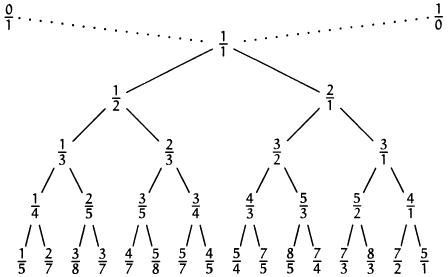
\includegraphics[scale=0.6]{2.jpg}

\subsubsection{ Proof }

\textbf{Orderliness.} It proved very simple: we note that the mediant of two fractions is always between them, i.e.:

$\frac {a} {b} \le \frac {a + c} {b + d} \le \frac {c} {d}$

provided that
$\frac {a} {b} \le \frac {c} {d}$

This can be proved simply bringing the three fractions to a common denominator.
Since the zero iteration ordering has taken place, it will continue to be true of every new iteration.

\textbf{Irreducible.} For this we show that for every iteration of any two adjacent fractions in the list $\frac {a} {b}$ and $\frac {c} {d}$ performed:

$bc-ad = 1$

Indeed, recalling the Diophantine equation with two unknowns($ax + by = c$ ), we deduce from this statement that ${\rm gcd} (a, b) = {\rm gcd} (c, d) = 1$ Which is what we needed.
So, we have to prove the truth of statements $bc-ad = 1$ for every iteration. We prove it also by induction. At zero iteration this property is satisfied (as is easily seen). Now, let it be done at the previous iteration, we show that it holds in the current iteration. For this we need to consider three fractions neighboring the new list:

$\frac {a} {b}, \frac {a + c} {b + d}, \frac {c} {d}$

For them, the conditions become:
$b (a + c) - a (b + d) = 1,$

$c (b + d) - d (a + c) = 1$

However, the truth of these conditions is obvious, if the truth $bc-ad = 1$. So really, this property holds for the current iteration, as required.
\textbf{Having all fractions.} The proof of this property is closely related to an algorithm to find the fraction in the Stern-Brocot tree. Given that the Stern-Brocot tree, all fractions in order, we find that for every vertex of the tree in the left subtree are a fraction smaller than it, and the right - most of it. And this gives us a clear shot of a search algorithm in the Stern-Brocot tree: first, we are in the root, compare our fraction and a fraction written in the current node: if the fraction is less than ours, then we go to the left subtree, if our shot more - go to the right, and if the same - find a fraction, the search is complete.

To prove that an infinite tree Stern-Brocot contains all the fractions, is sufficient to show that the ability to complete fractions in a finite number of steps for any given shot. This algorithm can be understood as follows: we have the current segment $\left [\frac {a} {b}; \frac {c} {d} \right]$ In which we are looking for our shot $\frac {x} {y}$. Initially $\frac {a} {b} = \frac {0} {1}$, $\frac {c} {d} = \frac {1} {0}$. At each step of the fraction $\frac {x} {y}$ compared with mediant endpoints, i.e. with $\frac {a + c} {b + d}$, And based on this we either stop the search, or go to the left or right side of the segment. If the search algorithm fraction worked endlessly, then the following conditions have been met for each iteration:

$\frac {a} {b} <\frac {x} {y} <\frac {c} {d}$

But they can be rewritten in the form:
$bx-ay \ge 1,$

$cy-dx \ge 1$

(Here we used the fact that they are integral, so from $> 0$ should $\ge 1$ )
Then, multiplying the first to $c + d$ And the second - on the $a + b$ And adding them, we get:

$(C + d) (bx-ay) + (a + b) (cy-dx) \ge a + b + c + d$

Expanding on the left and the fact that $bc-ad = 1$ (See the proof of the previous properties), we finally obtain:
$x + y \ge a + b + c + d$

And since each iteration at least one of the variables $a, b, c, d$ strictly increasing, the search for a fraction $\frac {x} {y}$ will contain no more than $x + y$ iterations, as required.
\subsubsection{ An algorithm for constructing the tree }

To build any subtree of the Stern-Brocot enough to know only the left and right of their ancestors. Initially, in the first level, the left is the ancestor $\frac {0} {1}$, And the right - $\frac {1} {0}$. They can be used to calculate the fraction in the current node, and then start from the left and right sons (left to his son passing itself as an ancestor of the right, and the rights to his son - as a left ancestor).

Pseudocode of the procedure, trying to build the infinite tree:

\begin{verbatim}
void build(int a = 0, int b = 1, int c = 1, int d = 0, int level = 1){
    int x = a + c,  y = b + d ;
    ... output current of the fraction x / y at the tree level
    build(a, b, x, y, level + 1);
    build(x, y, c, d, level + 1);
} 
\end{verbatim}
\subsubsection{ Search algorithm fraction }

The search algorithm fraction has already been described in the evidence that the Stern-Brocot tree contains all the fractions, we repeat it here. This algorithm - in fact, binary search, or search algorithm specified value in a binary search tree. Initially, we are at the root of the tree. Standing in the current node, we compare our fraction and a fraction in the current top. If they match, then the process stops - we found shot in the tree. Otherwise, if the fraction is less than our current fraction in the top, then go to the left child, otherwise - to the right.

As proved in the property that the Stern-Brocot tree contains all non-negative fractions, finding fractions $\frac {x} {y}$ algorithm will make no more $x + y$ iterations.

We present an implementation that returns the path to the top, containing a given fraction $\frac {x} {y}$, Returning it to a sequence of characters 'L' / 'R': if the current character is 'L', then it indicates a transition to a tree in the left child, and otherwise - in the right (initially we are at the root of the tree, i.e., at the top of a fraction $\frac {1} {1}$ ). In fact, a sequence of characters that uniquely identifying existing and any non-negative fraction, the \textbf{number system} is called \textbf{the Stern-Brock.}

\begin{verbatim}
string find(int x, int y, int a = 0, int b = 1, int c = 1, int d = 0){
    int m = a + c,  n = b + d ;
    if(x == m && y == n )
        return "" ;
    if(x * n < y * m )
        return 'L' + find(x, y, a, b, m, n);
    else
        return 'R' + find(x, y, m, n, c, d);
} 
\end{verbatim}
Irrational number in a Stern-Brocot correspond infinite sequence of characters, if known any desired degree of accuracy, we can limit some of the prefix of the infinite sequence. In the course of this endless search irrational fractions in the Stern-Brocot tree algorithm will be every time there is a simple fraction (with gradually increasing denominators), which provides a better approximation of the irrational number (it is important to use just in time techniques, and in this regard, and Achilles Brokaw discovered this tree.)

\subsection{ Farey sequence }

Farey sequence of order $n$ The set of all irreducible fractions between 0 and 1 whose denominators do not exceed $n$, The fractions are arranged in ascending order.

This sequence is named after the English geologist John Farey (John Farey), who attempted in 1816 to prove that in some Farey any fraction is the mediant of the two neighbors. As far as we know, the proof was wrong and correct proof offered later Cauchy (Cauchy). However, even in 1802, the mathematician Haros (Haros) in one of his works came to almost the same results.

Farey sequences and have many interesting properties of its own, but the most obvious their \textbf{relationship to the Stern-Brocot tree:} in fact, Farey sequence is obtained by removing some of the branches of the tree. Or we can say that for Farey sequence must take a lot of fractions obtained in the construction of the Stern-Brocot tree on the infinite iteration, and leave this set only fractions with denominators not exceeding $n$ and numerators, denominators do not exceed.

Of the algorithm for constructing the tree Stern-Brocot follows the same \textbf{algorithm} for Farey sequences. At zero iteration include in the set only a fraction $\frac {0} {1}$ and $\frac {1} {1}$. At each iteration, we next between each insert their mediant fractions, if the denominator does not exceed $n$. Sooner or later in the set no longer be any changes, and the process can be stopped - we found the desired sequence Farey.

Compute the \textbf{length of the} sequence Farey. Farey sequence of order $n$ contains all the elements of the sequence order Farey $n-1$ And all irreducible fractions with denominators equal $n$, But this number is known to be equal $\phi (n)$. Thus, the length $L_n$ Farey sequence of order $n$ expressed by the formula:

$L_n = L_ {n-1} + \phi (n)$

or revealing recursion:
$L_n = 1 + \sum_ {k = 1} ^ n \phi (k)$

\subsection{ Literature }

Ronald Graham, Donald Knuth, and Oren Patashnik. \textbf{Concrete Mathematics.} \textbf{Foundation of computer science} [1998]

\section{ Maximum segment sum }
Here we consider the problem of finding subsegments array with a maximum amount ("maximum subarray problem" in English), as well as some of its variations (including the algorithm for this problem in the version online - described by the author of the algorithm - KADR (Jaroslav Tverdokhleb)).

\subsection{ Statement of the problem }

Given an array of numbers $a [1 \ldots n]$. It is required to find a subsegment $a [l \ldots r]$ That amount to \textbf{its} highest:

$\max_{1\le l\leq r\leq n}\sum_{i=l}^{r}a[i]$

For example, if all of the array $a []$ would be non-negative, then the response would be to take the whole array. The solution is non-trivial when the array can contain both positive and negative numbers.

It is clear that the problem of finding \textbf{the minimum} subsegments - essentially the same, you just change the signs of all the numbers are reversed.

\subsection{ Algorithm 1 }

Here we consider virtually obvious algorithm. (Here we consider a different algorithm, which is slightly more difficult to come up with, but its implementation gets even less.)

\subsubsection{ Description of the algorithm }

The algorithm is quite simple.

For convenience we introduce \textbf{the notation:} $s [i] = \sum_ {j = 1} ^ {i} a [j]$. Ie array $s [i]$ - Is an array of partial sums array $a []$. Also set the value of $s [0] = 0$.

We will now \textbf{look over} the index $r = 1 \ldots n$ And learn the current value of each $r$ quickly find the optimum $l$, At which the maximum amount on the subsegments $[l; r]$.

Formally, this means that we need for the current $r$ find a $l$ (Not exceeding $r$)To the value $s [r] - s [l-1]$ was the highest. After a trivial transformation, we find that we need to find the minimum value in the array $s []$ minimum interval $[0; r-1]$.

Hence, we immediately obtain an algorithm solution: we simply store where the array $s []$ is the current minimum. Using this minimum, we are for $O (1)$ find current best index $l$, And the transition from the current index $r$ to the next, we simply update this minimum.

Obviously, this algorithm works for $O (n)$ and asymptotically optimal.

\subsubsection{ Implementation }

For implementation we do not even need to explicitly store an array of partial sums $s []$ - From it we will be required to the current element.

The implementation is in the 0-indexed arrays, but not in 1-numbering, as described above.

We first present a solution that has a simple numerical answer, finding the desired segment indices:

\begin{verbatim}
int ans = a[0],
    sum = 0,
    min_sum = 0 ;
for(int r = 0 ; r < n ; ++ r){
    sum + = a[r];
    ans = max(ans, sum - min_sum);
    min_sum = min(min_sum, sum);
} 
\end{verbatim}
Now for a full version of the solutions, which are parallel with the numerical solution is the boundary of the desired segment:

\begin{verbatim}
int ans = a[0],
    ans_l = 0,
    ans_r = 0,
    sum = 0,
    min_sum = 0,
    min_pos = - 1 ;
for(int r = 0 ; r < n ; ++ r){
    sum + = a[r];
 
    int cur = sum - min_sum ;
    if(cur > ans){
        ans = cur ;
        ans_l = min_pos + 1 ;
        ans_r = r ;
    }
 
    if(sum < min_sum){
        min_sum = sum ;
        min_pos = r ;
    }
} 
\end{verbatim}
\subsection{ Algorithm 2 }

Here we consider a different algorithm. Its a little more complicated to understand, but it is more elegant than the above, and realized a little shorter. This algorithm was proposed by Jay Kadan (Jay Kadane) in 1984

\subsubsection{ Description of the algorithm }

The \textbf{algorithm} is as follows. We will go through the array and store in a variable $s$ current partial sum. If at any time $s$ is negative, then we simply assign $s = 0$. States that the maximum of all values ​​of the variable $s$ That occurred during the work, and will answer to the problem.

\textbf{We prove} this algorithm.

Indeed, consider the first time when the amount of $s$ was negative. This means that, starting with zero partial sum, we eventually came to a negative partial sum - hence, all the prefix of the array, as well as any of its suffix have a negative amount. Consequently, all this prefix array will no longer be any good: it can only increase to a negative answer.

But this is not enough to prove the algorithm. In the algorithm we actually limit ourselves to find the answer to only those segments that begin immediately after the seats when the event $s <0$.

But, in fact, consider an arbitrary interval $[l; r]$, And $l$ not in a "critical" position (i.e. $l> p +1$ Where $p$ - The latter is a position in which $s <0$ ). Since the last critical position is strictly earlier than $l-1$, It turns out that the amount of $a [p +1 \ldots l-1]$ nonnegative. This means that by moving $l$ to position $p +1$ We will increase the response or, at least, do not change it.

One way or another, but it turns out that the answer is really in the search can be limited only by segments, starting immediately after the positions, which have an $s <0$. This proves the correctness of the algorithm.

\subsubsection{ Implementation }

As in Algorithm 1, we present the first simplified implementation, which searches only for a numeric answer, finding the boundaries of the desired segment:

\begin{verbatim}
int ans = a[0],
    sum = 0 ;
for(int r = 0 ; r < n ; ++ r){
    sum + = a[r];
    ans = max(ans, sum);
    sum = max(sum, 0);
} 
\end{verbatim}
A full version of solutions, maintaining the index of the desired segment boundaries:

\begin{verbatim}
int ans = a[0],
    ans_l = 0,
    ans_r = 0,
    sum = 0,
    minus_pos = - 1 ;
for(int r = 0 ; r < n ; ++ r){
    sum + = a[r];
 
    if(sum > ans){
        ans = sum ;
        ans_l = minus_pos + 1 ;
        ans_r = r ;
    }
 
    if(sum < 0){
        sum = 0 ;
        minus_pos = r ;
    }
} 
\end{verbatim}
\subsection{ Related tasks }

\subsubsection{ Find maximum/minimum subsegments with restrictions }

If in the problem to the desired length $[l; r]$ additional restrictions (for example, the length $r-l +1$ segment must be within specified limits), the algorithm described above is likely to be easily generalized to these cases - either way, the problem will continue to be to find a minimum in the array $s []$ for given additional restrictions.

\subsubsection{ The 2D case of the problem: finding the maximum / minimum submatrix }

This article describes the problem naturally generalizes to large dimensions. For example, in two dimensions, it turns into a search for such a submatrix $[l_1 \ldots r_1; l_2 \ldots r_2]$ given matrix, which is the maximum amount of numbers in it.

Of the above solutions for the one \textbf{easy to get a} solution for $O (n ^ 3)$ : Iterate through $l_1$ and $r_1$, And calculate the sums from an array of $l_1$ on $r_1$ in each row of the matrix, we have come to a one-dimensional problem of search indexes $l_2$ and $r_2$ in the array, which can already be solved in linear time.

\textbf{Faster} algorithms for the solution of this problem although known, but they are not much faster $O (n ^ 3)$ And at this very difficult (so complex that the hidden constant, many of them inferior trivial algorithm for any reasonable restrictions). Apparently, the best known algorithms for working $O \left (n ^ 3 \frac {\log ^ 3 \log n} {\log ^ 2 n} \right)$ (T. Chan 2007 "More algorithms for all-pairs shortest paths in weighted graphs").

This algorithm Chan, as well as many other results in this area actually document \textbf{the rapid multiplication of} matrices (where the matrix multiplication means multiplying modified: instead of adding at least used, and instead of multiplication - addition). The fact that the problem of finding the submatrix with the largest sum is reduced to the problem of finding the shortest paths between all pairs of vertices, and this problem in turn - is reduced to the matrix multiplication.

\subsubsection{ Find maximum / minimum average subsegments }

This problem lies in the fact that we must find a segment $[l; r]$ To mean it was the highest:

$\max_{l\leq r}\frac{1}{r-l+1}\sum_{i=l}ra[i]$

Of course, if the desired segment $[l; r]$ by the condition of the other conditions are imposed, the decision will always be a segment of length $1$ at the maximum of the array. The problem makes sense only if there are \textbf{additional restrictions} (for example, the length of the desired segment is bounded below).

In this case we can apply \textbf{the standard method} when dealing with tasks of secondary importance: we select the desired maximum average \textbf{binary search.}

To do this, we need to learn how to solve a subproblem: given the number of $x$, And you should check whether the array subsegment $a []$ (Of course, meeting all additional restrictions of the problem), which mean more $x$.

To solve this subproblem, subtract $x$ from each element of the array $a []$. Then our subproblem actually turns into this: whether or not in the array subsegment positive amount. And this problem we can solve.

So we got the solution for the asymptotic $O (T (n) \log W)$ Where $W$ - The required accuracy, $T (n)$ - Time subproblem solutions for an array of length $n$ (Which can vary depending on the specific additional restrictions).

\subsubsection{ Solution to the online problem }

Condition of the problem is: given an array of $n$ numbers, along with a number of $L$. Enter a query such as $(l, r)$ And in response to a query you want to find the segment subsegment $[l; r]$ length at least $L$ with maximum average.

Algorithm for this problem is quite complex. By this algorithm - KADR (Jaroslav Tverdokhleb) - the algorithm described in his forum post.
